
%%%%%%%%%%%%%%%%%%%%%%%%%%%%%  PREAMBLE  %%%%%%%%%%%%%%%%%%%%%%%%%%%%%

\documentclass[12pt,a4paper,openany]{book}

\usepackage{preamble}


%%%%%%%%%%%%%%%%%%%%%%%%%%%%%  DOCUMENT  %%%%%%%%%%%%%%%%%%%%%%%%%%%%%

\begin{document}

% Boldface proof name
% \let\oldproofname=\proofname
% \renewcommand{\proofname}{\rm\bf{\oldproofname}}

% PORTADA/PREFACIO/ÍNDICE --------------------------------------------
\frontmatter
\pagenumbering{roman}

% Portada
\begin{titlepage}
\newgeometry{top=4cm, bottom=3.5cm, left=3cm, right=3cm}
%
\centering
%
    {\includegraphics[width=0.2\textwidth]{Figures/LogoUsal.pdf}\par}
%
\vspace{.5cm}
% 
    {\bfseries\Large Universidad de Salamanca \par}
    \vspace{.3cm}
    {\scshape\large Facultad de Matem\'aticas \par}
%
\vspace{4cm}
%
    {\scshape\Huge Ampliación de Álgebra Conmutativa \par}
    \vspace{.5cm}
    {\itshape\LARGE \thetitle \par}
%
    \vfill
%
     {\large \theauthor  \\
    Clases impartidas por Carlos Sancho de Salas \par}
    \vspace{1cm}
    {\Large \thedate \par}
%
\restoregeometry
\end{titlepage}



\tableofcontents

% Prefacio
%
\chapter*{Prefacio} 

\justifying La Geometría Proyectiva nació como solución a los problemas de perspectiva que
aparecen al tratar de representar en un plano objetos del espacio. Este tipo de necesidades, surgidas en la pintura y arquitectura, llevaron a la creación de una teoría
matemática que recogiera las bases geométricas subyacentes a los métodos concretos
que poco a poco se fueron elaborando en esos campos del arte.

Las primeras ideas de geometría proyectiva se remontan al Renacimiento motivadas
por la actividad de artistas y arquitectos. Piero della Francesca (1410-1492), Leone
Battista Alberti (1404-1472) y Alberto Durero (1471-1528) reflexionaron sobre nociones
geométricas como las de proyección y sección para entender el problema de la representación de un objeto real tridimensional en un lienzo plano. El primer matemático
que hizo uso de esas ideas fue el francés Girard Desargues (1591-1661), que introdujo los métodos proyectivos en su estudio de las cónicas. Nociones proyectivas como
los puntos del infinito fueron introducidos por Desargues al mismo tiempo que nuevos
métodos de demostración, que le permitieron realizar el mayor avance en el estudio
de las cónicas desde los tiempos de Apolonio. Mientras que los griegos tenían que
idear un método diferente para cada teorema particular, Desargues vio en el enfoque
proyectivo un procedimiento general que le permitía establecer resultados para todas
las cónicas. Desargues influyó fuertemente sobre Blaise Pascal (1623-1662) y Philippe
de la Hire (1640-1718), que dedicaron una actividad considerable al estudio proyectivo
de las cónicas.
 
La Geometría Proyectiva estudia las propiedades de las figuras que se conservan por
proyección. Así, los matemáticos anteriormente mencionados enunciaron nuevos teoremas en los que nociones geométricas clásicas como longitud y ángulo eran sustituidas
por otras de incidencia de las figuras que, a diferencia de las primeras, sí se conservaban por proyección. Progresivamente se fue haciendo claro que los métodos basados en
estas ideas eran mucho más generales que los tradicionales y, a partir de una cuidadosa
distinción entre las propiedades proyectivas y las métricas, a finales del siglo XIX se
configuró una geometría mucho más amplia, la Geometría Proyectiva, que engloba a
todas las geometrías conocidas anteriormente. Esto es, las geometrías afín, euclídea y
no euclídeas se pueden considerar subgeometrías de la proyectiva. Un ejemplo claro
de este hecho es el modelo de geometría hiperbólica que proporciona la Geometría
Proyectiva especialmente adecuado para tener una visión intuitiva de dicha geometría
no euclídea.

Por otro lado, en la Geometría Proyectiva se ha desarrollado la noción de transformación que, a partir de las ideas presentadas por Felix Klein (1849-1925) en su “programa
de Erlangen”, ocupa un lugar central en la construcción de cualquier teoría geométrica.
De esta forma, el concepto de invarianza por transformaciones, que tan importante ha 
sido en la física moderna, ha sido largamente anticipado en la Geometría Proyectiva
al estudiar las propiedades geométricas que permanecen invariantes por cambios de
coordenadas.

Dentro del cuerpo de las matemáticas, la Geometría Proyectiva se puede considerar
como un modelo de teoría que teniendo sus orígenes en el mundo real, llega a un
nivel de elaboración en el que se combinan “la perfección formal, la elegancia en el
razonamiento y la riqueza de las intuiciones”.
Hay que destacar que a principios del siglo XIX, la presentación que se hizo de la
Geometría Proyectiva fue de tipo sintético o axiomático. Una de las figuras más importantes fue Jean-Victor Poncelet (1788-1867), que estudió las figuras homólogas, es decir,
relacionadas entre sí a través de proyecciones y secciones, dando la definición de transformación proyectiva como aquellas aplicaciones que son composición de proyecciones
o perspectividades. Otra figura importante fue Karl G. C. von Staudt (1798-1867),
quien contribuyó de modo significativo a establecer los fundamentos de la Geometría
Proyectiva, haciéndola independiente de las nociones de longitud, distancia y ángulo
y, por tanto, aclarando desde un punto de vista lógico que la Geometría Proyectiva es
anterior a la euclídea. Además, las transformaciones proyectivas que consideró fueron
las aplicaciones biyectivas que transforman 3 puntos alineados en tres puntos alineados,
conocidas también como colineaciones.

La introducción de las ideas algebraicas en geometría proyectiva tuvo lugar también en esas fechas. Sus impulsores fueron Augustus F. Möbious (1790-1868) y Julius Plücker (1801-1868). Ellos fueron los primeros en usar las coordenadas homogéneas para formular algebraicamente muchas ideas proyectivas. A finales del siglo XIX, con
las ideas de la geometría moderna, se consiguió que las demostraciones con cálculos en coordenadas desaparecieran de la geometría proyectiva y se impusieran los razonamientos puramente lógicos a través del álgebra lineal. En estos apuntes, comenzaremos con la presentación algebraica de la Geometría Proyectiva a partir de las rectas que pasan por el origen de un espacio vectorial. Posteriormente veremos la presentación axiomática, quizás más intuitiva desde el punto de vista de una geometría formal, y finalmente comentaremos la equivalencia de las dos presentaciones para el caso del plano proyectivo, construyendo el cuerpo de escalares a partir de propiedades geométricas como el teorema de Desargues y el teorema de Pappus. En esta equivalencia es donde se aprecia la importancia del “Teorema Fundamental de la Geometría Proyectiva”, el cual afirma que las transformaciones de las dos geometrías, algebraica y axiomática, son las mismas.

\hfill Esteban Gómez. 4 de abril de 2003.
\cleardoublepage

% Índice
\let\cleardoublepage\clearpage %quita la página en blanco

% CUERPO -------------------------------------------------------------
\mainmatter
\pagenumbering{arabic}
\fancychapterstyle

\chapter{Completaci\'on de m\'odulos} \justifying
Sea $X$ un conjunto
\begin{defi}
Una \textbf{pseudom\'etrica} es una aplicaci\'on
$$\bt  d: X \times X \rar & \bb R^+ \\[-5mm] (x,y) \rarmaps & d(x,y) \et$$
con la propiedades sim\'etrica, reflexiva y triangular
$$d(x,y) = d(y,x) \qquad d(x,x)=0 \qquad d(x,y) \le d(x,z) + d(z,y)$$
que definen bolas 
$$B_{\varepsilon}(x) = \{y\in X \, /\, d(x,y) < \varepsilon\} \quad \varepsilon > 0$$ que a su vez definen la \textbf{topolog\'ia de las bolas}, cuyos abiertos son uni\'on de bolas. Construimos as\'i el espacio topol\'ogico $(X,\mc U_d)$ asociado a la pseudom\'etrica $(X,d)$. 
\end{defi}
\begin{obs}
    Para que una psudeom\'etrica sea m\'etrica hace falta que 
    $$d(x,y) = 0 \iff x=y$$
\end{obs}
\begin{prop}
    $(X,d)$ es m\'etrico $\iff (X,\mc U_d)$ es separado ($= T_2$). 
\end{prop}
\begin{dem}
    $\Rightarrow)$ Definiendo $\bar d = d(x,y)$ y las bolas $B_{\nicefrac{1}{3} \bar d} (x)$, $B_{\nicefrac{1}{3}\bar d} (y)$, no existe $z$ en ambas bolas pues contradir\'ia la desigualdad triangular.

    $\Leftarrow)$ Para cada $y\in X$ podemos encontrar $B_{\varepsilon}(x) \ni y$. 
\end{dem}
Sea $(X,d)$ un espacio pseudom\'etrico y $\big\{\{x_n\}_{n\in \bb N}\big\}$ el conjunto de las sucesiones en $X$, y consideramos $\mc C \subset Suc(X)$ las sucesiones de Cauchy, es decir, que verifican que
\begin{defi}
    $\{x_n\}$ es una \textbf{sucesi\'on de Cauchy} si para cada $\varepsilon \in\bb R^+$ existe $n_o \in \bb N$ tal que $$d(x_n,x_m)< \varepsilon \qquad \forall \, n,m \ge n_o$$ 
    Intuitivamente decimos que estas sucesiones convergen.
\end{defi}
\begin{defi}
    Dos \textbf{sucesiones de Cauchy} $\{x_n\} \sim \{y_n\}$ se dicen \textbf{equivalentes}, y se denota por $\{x_n\} \sim \{y_n\}$, si $\{d(x_n,y_n)\}$ es una sucesi\'on de Cauchy convergente a 0.
\end{defi}
\begin{defi}
    La \textbf{completaci\'on} de $(X,d)$ es el conjunto 
    $$\widehat X = \modulo{\text{Sucesiones de Cauchy}}{\sim}$$
\end{defi}
\begin{ejem}
    $\widehat {\bb Q} = \bb R$
\end{ejem}
\begin{prop}
    $(X,d) \longrightarrow (\widehat X, \widehat d)$ define una isometr\'ia de forma que $(\widehat X, \widehat d)$ es un espacio m\'etrico. Se define
    $$\bt  X \rar{\varphi} & \widehat X \\[-5mm] x \rarmaps & \{x\}_{n\in \bb N} \et$$
    y la distancia $\widehat d$ es 
    $$\widehat d\big([\{x_n\}],[\{y_n\}]\big) = \lim_{n\to \infty} d(x_n,y_n)$$
    de forma que hay que comprobar que si $[\{x_n\}], [\{y_n\}]$ son sucesiones de Cauchy, $d(x_n,y_n)$ es una sucesi\'on de Cauchy convergente, que existe ese l\'imite y no depende de los representantes, y adem\'as que verifica las propiedades de distacia. 

    El nuevo espacio m\'etrico $(\widehat X, \widehat d)$ es completo, toda sucesi\'on de Cauchy converge. 

    La isometr\'ia es inyectiva ($(X,d) \hookrightarrow (\widehat X, \widehat d)$) si y solo si $d$ es m\'etrica. 

    $(\widehat X, \widehat d)$ ya es m\'etrico pues $d(x,y) = 0 \iff \{x\} \sim \{y\}$.
\end{prop}
\begin{cor}
    Concluimos as\'i que todo espacio psuedom\'etrico se sumerge en un espacio m\'etrico completo, y es el m\'inimo, es decir, si $(X,d) \hookrightarrow (\widehat Y, \bar d)$ (con $\widehat Y$ otro espacio completo), entonces factoriza
    $$\bt (X,d) \rar[hook] \arrow{d} & (\widehat X, \widehat d) \arrow{dl} \\[5mm] (\widehat Y, \bar d) \et$$
    Es decir, $$Hom_{unif}((X,d), \widehat Y) = Hom_{unif} (\widehat X_d, \widehat Y)$$
\end{cor}
\begin{prop}
    Sea $(E,+)$ un grupo abeliano, consideremos pseudom\'etricas $d$ tales que $d(e+\bar e, e'+\bar e) = d(e,e')$. De forma que dar $d(0,e)=\|e\|$ es dar todas las distancias $d(e,\bar e) = d(0,e-\bar e)$. Se tiene tambi\'en la propiedad triangular, sim\'etrica y reflexiva 
    $$\|e+e'\|\le \|e\|+\|e'\| \qquad \|\lambda e\| = |\lambda| \|e\| \qquad \|e-e'\| = \|e'-e\|$$
\end{prop}
\begin{obs}
    Dadas dos distancias $d,d'$ si para cada $\varepsilon \in \bb R^+$ existe $\delta\in \bb R^+$ con 
    $$d(x,y) <  \delta \Rightarrow d'(x,y) < \varepsilon \quad  \equiv \quad B_{\delta}^d(x) \subset B_{\varepsilon}^{d'}(x) $$
    (que $d$ es m\'as fina que $d'$) y si se cumple tambi\'en que 
    $$d'(x,y) <  \delta' \Rightarrow d(x,y) < \varepsilon' \quad  \equiv \quad  B_{\delta'}^{d'}(x) \subset B_{\varepsilon'}^d(x)$$
    estas distancias definen la misma topolog\'ia, y ambas definen las mismas sucesiones de Cacuhy. 
\end{obs}
\section{Filtraciones}
Sea $M$ un $A$-m\'odulo, 
\begin{defi}
    Una \textbf{filtraci\'on en} $M$ es una cadena 
    $$M =M_o \supset M_1\supset M_2 \supset \cdots\supset M_n \supset \cdots \supset 0$$
\end{defi}
\begin{defi}
    Se define la \textbf{distancia} entre dos elementos de la \textbf{filtraci\'on}
    $$d(m,m') = \begin{cases}
        \dfrac{1}{2^i} & \text{ si } m-m'\in M_i - M_{i+1} \\[3mm] 0 & \text{ si } m-m'\in\displaystyle \bigcap_i M_i 
    \end{cases}$$
\end{defi}
\begin{prop} \,
    \begin{enumerate}[1)]
        \item $d$ es pseudom\'etrica en $M$.  
        \item $d$ es m\'etrica $\iff$ $\displaystyle \bigcap_{i\in \bb N} M_i = 0$
    \end{enumerate}
\end{prop}
\begin{defi}
    Se tiene as\'i en $M$ una topolog\'ia y se define $\widehat M$ el \textbf{completado de} $M$ por $\{M_i\}_{i \in \bb N}$. 
\end{defi}
\begin{prop}
    Dos filtraciones $\{M_i\}_{i \in \bb N}$, $\{M'_i\}_{i \in \bb N}$ definen m\'etricas equivalentes $\iff$ para cada $n \in \bb N $, existe $n_o$ tal que
    $$M_{n_o} \subset M_n'$$
    y rec\'iprocamente, para cada $n \in \bb N$ existe $n_o \in \bb N$ tal que 
    $$M_{n_o}' \subset M_n$$
\end{prop}
\begin{dem}
    Al lector.
\end{dem}
Sea $I$ un conjunto parcialmente ordenado de \'indices filtrante decreciente.
\begin{defi}
    Un \textbf{sistema proyectivo} es una familia de m\'odulos $\{\bar M_i\}_{i \in I}$ y para cada $i \le j$,  $\varphi_{ij} : \bar M_i \longrightarrow \bar M_j$ verficando que para cada $i \le j \le k$
    $$\bt \bar M_i \rar{\varphi_{ij}} \arrow[bend right=10mm]{rr}{\varphi_{ik}}& \bar M_j \rar{\varphi_{jk}} \rar & \bar M_k \et \qquad \boxed{\varphi_{ik} = \varphi_{jk} \circ \varphi_{ij}}$$
    \end{defi}
\begin{ejem}
     Podemos usar los naturales como \'indices $I = \bb N$, pero invertimos el orden para que sea filtrante decreciente, para cada $i,j \in I$ existe otro $k \le i,j$ con
     $$\bt \cdots \rar{\varphi_{43}} & M_3 \rar{\varphi_{32}} & M_2 \rar{\varphi_{21}} & M_1\et$$
\end{ejem}
\begin{defi} Se define el \textbf{l\'imite proyectivo} del sistema proyectivo como
    $$\varprojlim M_i = \left\{(m_i)_{i \in I} \in \prod M_i \, / \, \varphi_{ij}(m_i) = m_j \text{ si } i \le j \right\} $$
\end{defi}
\begin{obs}
    Si $I=\bb N$, intuitivamente
    $$\bt \varprojlim M_i \rar 
    &\cdots \rar{\varphi_{43}} & M_3 \rar{\varphi_{32}} & M_2 \rar{\varphi_{21}} & M_1\et$$
\end{obs}
\begin{prop}
    $\varprojlim M_i \subset \prod M_i$ es un subm\'odulo, que induce
    $$\bt \varprojlim M_i \subset \rar[hook] \arrow{dr}{\varphi_i} & \prod M_i \arrow{d}{\pi_i} \\[5mm] & M_i \et$$
    y se tienen los tri\'angulos conmutativos
    $$\bt \varprojlim M_i \subset \rar{\varphi_i} \arrow{dr}{\varphi_j} & \prod M_i \arrow{d}{\varphi_{ij}} \\[5mm] & M_j \et \qquad \text{ si }i \le j$$
\end{prop}
\begin{propi}
    [Universal] Se tiene que 
    $$Hom_A(N,\varprojlim M_i) = \varprojlim Hom_A(M,M_i)$$
    que nos dice que
    $$N \longrightarrow \varprojlim M_i \text{ es morfismo } \iff  \bt N \rar{T_i} \arrow[swap]{dr}{T_j} & M_i \arrow{d}{\varphi_{ij}} \\ & M_j \et \text{ es conmutativo.}$$
\end{propi}

Dada una filtraci\'on $M  = M_o \supset M_1 \supset \cdots \supset M_n \supset \cdots $ consideramos los cocientes
$$\cdots \longrightarrow \modulo{M}{M_2} \longrightarrow \modulo{M}{M_1} \longrightarrow \modulo{M}{M_o} = 0$$
siendo los morfismos las proyecciones naturales, que es un sistema proyectivo, y tiene por l\'imite proyectivo $\varprojlim \modulo{M}{M_i}$ y $M$ factoriza por \'el, no es igual a $M$ ni tampoco a $\modulo{M}{\bigcap M_i}$, es algo m\'as rico.

Se tienen los morfismos 
$$\bt \modulo{M}{M_j} \rar{\pi_{ij} } & \modulo{M}{M_i} \et \quad M_i \supset M_j  \text{ si } i \le j$$
y $[n_i]_i \in \modulo{M}{M_i}$, con $\pi_{ij}(m_j) = m_i \mod M_i$, $[m_{j}]_i = [m_i]_i$, por lo que se tiene el sistema proyectivo $(n_i)$ con $n_i - n_j \in M_i$ si $i\le j$.
\begin{teo}
    $\widehat M = \varprojlim \modulo{M}{M_i}$.
\end{teo}
\begin{lem}
    Sea $\{x_i\}_{i \in \bb N} \subset X$ una sucesi\'on de Cauchy, cualquier subsucesi\'on $\{x_{n_i}\}_{i \in \bb N} \subset \{x_n\}_{i \in \bb N}$ es de Cauchy y equivalente a $\{x_i\}_{i \in \bb N}$
\end{lem}
\begin{dem}
    Usar la convergencia de ambas, y la distancia entre ellas. 
\end{dem}
\begin{defi}
    Una \textbf{serie en la filtraci\'on} de una familia de elementos $\{m_i\}_{i \in \bb N}$ con $m_i\in M_i$ es la suma formal $$\sum_{i=0}^{\infty} m_i = \left( \sum_{i=0}^{n-1} m_i \right)_{n \in \bb N}$$
    y son siempre de Cauchy, pues 
    $$\sum_{i=0}^{n-1} m_i-\sum_{i=0}^{m-1} m_i = \sum_{i=m}^{n-1} m_i \in M_m \Rightarrow 
    d\left(\sum_{i=0}^{n-1} m_i, \sum_{i=0}^{m-1} m_i\right) \le \frac{1}{2^m} \qquad m \le n$$
\end{defi}
\begin{lem}
    Consideremos $\{M_i\}_{i \in \bb N}$ una filtraci\'on de $M$, toda sucesi\'on de Cauchy es equivalente a una serie, es decir, $\displaystyle (n_i)_{i \in \bb N} \sim \left( \sum_{i=0}^{\infty} m_i \right)$
\end{lem}
\begin{dem}
    $(n_i)_{i \in \bb N} $ de forma que para cada $i$ existe $j_i \in \bb N$ tal que $d(n_s,n_k) \le \frac{1}{2^i}$ con $s,k \ge j_i$. Escogemos entonces la subsucesi\'on $(n_{j_i})_{i \in \bb N}$, que por el primer lema es equivalente a la original. Si renombramos $(n_{i_j})_{i \in \bb N} = (\bar n_i)_{i \in \bb N}$, entonces 
    $$d(\bar n_i, \bar n_j) = d(n_{j_i}, n_{j_j}) \le \frac{1}{2^i} \Rightarrow \bar n_i -\bar n_j \in M_i \quad i \le j$$
    es decir, es una subsucesi\'on de forma que cada t\'ermino dista del siguiente lo justo para estar en $M_i$. 

    Por la teor\'ia de operadores, $\Delta \left(\sum _{0}^{n-1} m_i \right) = m_n$, $\Delta(\bar n_i) = \bar n_{i+1} - \bar n_i = m_i \in M_i$ es una sucesi\'on tal que el t\'ermino $i$-\'esimo est\'a en $M_i$. De forma que 
    $$\sum_{i=0}^{n-1}m_i = \bar n_n$$
    por tener las dos la misma diferencial, es decir, $$\bar n_n = \frac{1}{\Delta} (\Delta \bar n_n) = \frac{1}{\Delta} (\bar m_n) = \sum_0^{n-1} \bar m_i$$
    y como si dos series tienen la misma diferencial difieren una constante
    $$n_i = \frac{1}{\Delta} (\Delta n_i) + n_o' = \frac{1}{\Delta}(m_i) + n_o' = \sum_{j=0}^{i-1} m_j  + n_o' = \sum_{j=0}^{i-1} m_j \qquad (\text{tal que } m_o = m_o + n_o')$$ 
    damos valor cuando $n=1$, $\bar m_o = (\Delta \bar n_m )_o = \bar n_1 - \bar n_o$ y redefinimos la serie como $n_o+ \sum_{0}^{\infty} \bar m_o$.  

    Y toda sucesi\'on de Cauchy es equivalente a una serie, $\sum_0^{n-1} m_i = \bar n_n$
\end{dem}
\begin{dem}[del Teorema]
    Se tiene $M \longrightarrow \modulo{M}{M_i}$, veamos qu\'e hacemos corresponder a qu\'e. Recordemos que $\widehat M = \{[(n_i)_{i \in \bb N}] \text{ de Cauchy}, n_i \in M\}$ y 
    $$\varprojlim \modulo{M}{M_i} = \{([\bar n_i])_{i \in \bb N} \, / \, \bar n_i - \bar n_j \in M_j \text{ si } i \ge j \}$$ 
    $$\bt \widehat M \rar & \varprojlim \modulo{M}{M_i}  \\[-5mm] (n_i)_{i\in I} = (\sum^{i-1} m_j) \rarmaps & \left(\left[\sum_{j=0}^{i-1} m_j \right]_i\right) \et$$
    y 
    $$\bt \modulo{M}{M_i} \rar & \modulo{M}{M_{i-1}} \\[-5mm] [\sum^{i-1} m_j ]\rarmaps & [\sum^{i-2}m_i] = [\sum^{i-1} - m_{i-1}] \et$$
    y del rev\'es, $(n_i)$ va a parar a $n_i = n_{i-1} \mod M_{i-1}$, de forma que $([n_i])$ es de Cacuhy, y 
    $$\bt \widehat M \rar & \varprojlim \modulo{M}{M_i}  \\[-5mm] (n_i) & \arrow[mapsto]{l} ([n_i]) \et$$ 
\end{dem}

Dado un $A$-m\'odulo $M$ y una filtraci\'on $M = M_o \supset M_1 \supset \cdots \supset M_i \supset \cdots$, que define una pseudom\'etrica con una distancia $d(m,m') \le \frac{1}{2^i}, \, m-m'\in M_i$, y se pueden hablar de las sucesiones de Cacuhy, y que son equivalentes cuando la distancia entre los t\'erminos de las dos sucesiones tiende a 0, definiendo as\'i el completado de $M$, $\widehat M$. De forma que si $\{n_i\}$ es de Cauchy, $\{n_i'\}$ otra, $n_i' - n_{i+1} \in M_i$, lo que permite demostrar la igualdad
$$\bt \widehat M \rar[equal] & \varprojlim \modulo{M}{M_i} \\[-5mm] (n_i)_{i \in I} \rarmaps & (\bar n_i)_{i \in \bb N} \\[-5mm](n_i)_{i \in I} & \arrow[mapsto]{l} (\bar n_i) \et$$
siendo $\bar n_i$ la clase de $n_i \mod M_i$. Y del rev\'es, tal que la familia $(n_i)$ cumplan que $n_i-n_{i+1} \in M_i$.

Adem\'as, toda sucesi\'on de Cauchy es equivalente a una serie $\sum_i m_i$ con $m_i \in M_i$. De forma que el elemento $i$ es $\left( \left[\sum_j^{i-1} m_i \right]\right)_{i \in \bb N} $. De forma que se denota $(n_i)_{i \in \bb N} \sim \sum_{i=0}^{\infty} m_i$ y cada $n_i = n_{i-1} + m_{i-1} = n_{i-2} + m_{i-2} + m_{i-1} = \cdots  = \underbrace{n_o=m_o}_{\in M_o}+ m_1 + m_2 + \cdots + m_{i-1} $, que ahora ya es m\'etrica y se tiene el morfismo de completaci\'on 
$$\bt M \rar{\varphi} & \widehat M \\[-5mm] m \rarmaps & (m)_{i \in \bb N} \et \qquad \ker \varphi = \bigcap_{i \in I} M_i$$
\begin{ejem}
    Sea $A$ con $\alpha \subset A$ un ideal, $M$ un $A$-m\'odulo, escogemos la filtraci\'on $M_i = \alpha^n \cdot M $, es $$M_o = M \supset \alpha M \supset \alpha^2 M \supset \cdots \supset \alpha^n M \supset \cdots $$
\end{ejem}
\section{Exactitud de la completcai\'on}
Sea la sucesi\'on exacta de m\'odulos
$$\bt 0\rar & N \rar{i} & M \rar{\pi} & \bar M \rar & 0 \et$$
pudiendo identificar $N\subset M$ y $\bar M = \modulo{M}{N}$, y la filtraci\'on en $M$: $M  = M_o \supset M_1 \supset \cdots \supset M_n \supset \cdots$, tenemos filtraciones en $N$: $\{N \cap M_i\}_{i\in \bb N}$ y en $\bar M$: $\{\pi(M_i)\}_{i\in \bb N}$

\begin{teo} La sucesi\'on
$$\bt 0\rar & \widehat N \rar{\widehat i} & \widehat M \rar{\widehat \pi} & \widehat {\bar M} \rar & 0 \et$$
es exacta.
\end{teo}
\begin{obs}
    La exactitud se conserva por mantener las topolog\'ias inducidas en $N$ y $\bar M$ como cociente. 
\end{obs}
\begin{dem}
    $$\bt 0\rar & N \rar & M \rar{\pi} \arrow{dr} \arrow[squiggly]{d} & \bar M \arrow{d} \rar & 0 \\[5mm] 0 \rar & \modulo{N}{N \cap M_i} \rar & \modulo{M}{M_i} \rar{ \pi_i} & \modulo{\bar M}{\pi(M_i)}  \rar[dashed] & 0  \et$$
    de forma que 
    $$\ker \pi_i = \pi^{-1}_i (\pi(M_i)) = \modulo{M_i + N }{M_i} \simeq \modulo{N}{N \cap M_i}$$ 
    por ser $\pi^{-1}(\pi(N)) = M'+\ker \pi$. 

    El problema queda en la epiyectividad. 

    Para completar $\widehat {\bar M}$ escogemos elementos suyos, que son de la forma $[\sum_i\pi(m_i)]$ y $\widehat \pi$ identifica $[\sum m_i] \mapsto [\sum_i\pi(m_i)]$, pero no siempre es epiyectivo. 
\end{dem}
\begin{ejem}
    Volviendo al ejemplo de la filtraci\'on $\alpha$-\'adica, $N \cap \alpha^nM \supset \alpha^n N$ y esto hace que sea exacta, pues las completaciones son equivalentes. 
\end{ejem}
\begin{ejem}
    [Topolog\'ia y completaci\'on $\alpha$-\'adica] Sea $A$ anillo y $\alpha \subset A$ ideal, para un $A$-m\'odulo $M$ su topolog\'ia $\alpha$-\'adica es $\{\alpha^i \cdot M\}_{i \in \bb N}$. En particular, $\widehat A$ es anillo (producto de sucesiones, comprobar), y se tiene el morfismo de anillos
    $$\bt A \rar & \widehat A \\[-5mm] a \rarmaps & \left[(a)_{i \in \bb N} \right] \et$$
     de forma que $\widehat M$ no solo es $A$-m\'odulo, es tambi\'en $\widehat A$-m\'odulo con el producto
     $$(a_i)\cdot (n_i) = (a_i \cdot n_i)_i$$
     que no depende del representante elegido. 
\end{ejem} 
\begin{defi}
    Se dice que una filtraci\'on $\{M_i\}_{i \in \bb N}$ en $M$ es una \textbf{$\alpha$-filtraci\'on} si $\alpha M_i \supset M_{i+1} \, \forall \, i$. Llamaremos \underline{la} $\alpha$-filtraci\'on a $M\supset \alpha M \supset \cdots \supset \alpha^i M \supset \cdots$, que tambi\'en llamaremos can\'onica. Se dice que una $\alpha$-filtraci\'on es \textbf{$\alpha$-estable} si $\alpha M_i = M_{i+1}$ con $i\ge n_o$. 
\end{defi}
\begin{lem}
    Las $\alpha$-filtraciones son equivalentes a \underline{la} $\alpha$-filtraci\'on. Si $\{M_i\}_{i \in \bb N}$ es $\alpha$-estable, entonces $\{M_i\}_{i \in \bb N}\sim \{\alpha^i M\}_{i \in \bb N}$. 
\end{lem}
\begin{dem}
    Por ser $\{M_i\}_{i \in \bb N}$ una $\alpha$-filtraci\'on, entonces, $\alpha^i M =\alpha^iM_o \subset M_i \forall \, i$. 

    Para la inclusi\'on contraria, cada $M_i \subset M_o =M$ a partir de cierto $i$. Consideramos $n_o \in I$ y como $\alpha M_i = M_{i+1}$, es decir, $M_{n_o+h} \subset \alpha^h M$, porque $M_{n_o} \subset M \Rightarrow M_{n_o+h} = \alpha^h M_{n_o} \subset \alpha^h M$.  
\end{dem}
\begin{defi}
    Sea $A$ anillo e $\alpha$ ideal de $A$, definimos el \textbf{dilatado de }$A$ \textbf{por} $\alpha$ como
    $$D_{\alpha} A = A \oplus \alpha \oplus \alpha^2 \oplus \cdots  \oplus \alpha^i \oplus \cdots = A[t\alpha] $$
    que es una $A$-\'algebra graduada. Y sus elementos son de la forma $ \displaystyle \sum_i t^i \alpha_i, \, \alpha_i \in \alpha^i =\bigoplus_i \alpha_i$ y con el producto usual de polinomios.
\end{defi}
\begin{prop}
    Si $\alpha$ es finito generado, $\alpha=(a_1, \ldots, a_n)$, entonces $$ \bt A[x_1, \ldots, x_n] \rar & D_{\alpha} A \arrow{rr} &[-13mm] & 0 \\[-5mm] x_1, \ldots, x_n \rarmaps & \alpha_1, \ldots, \alpha_n &[-13mm] \in 0 \oplus \alpha \oplus 0 \oplus \cdots   \et$$
\end{prop}
Sea $A$ anillo, $\alpha \subset A$ finito generado y $M$ un $A$-m\'odulo finito generado,
\begin{teo}
    Una $\alpha$-filtraci\'on $\{M_i\}_{i \in \bb N}$ de m\'odulos finito generados es estable si y solo si
    $$DM = M \oplus M_1 \oplus M_2 \oplus \cdots \oplus M_i \oplus \cdots $$
    es un $D_{\alpha}A$-m\'odulo finito generado. 
\end{teo}
\begin{dem}
    $\Rightarrow) \, \alpha M_i = M_{i+1}$ para cierto $i \ge n_o$ y $M_{n_o+h} = \alpha^h M_{n_o}$, $M_o\oplus M_1 \oplus \cdots \oplus M_{n_o}$ genera $\bigoplus_i M_i$ como $D_{\alpha}A$-m\'odulo (por ejemplo $\cdots \oplus 0\oplus M_{n_o+h} \oplus 0 \oplus \cdots= (\cdots \oplus 0\oplus \alpha_h \oplus 0 \oplus \cdots)(\cdots \oplus 0\oplus M_{n_o} \oplus 0 \oplus \cdots)$). Por tanto, $M_o\oplus M_1 \oplus \cdots \oplus M_{n_o}$ es un $A$-m\'odulo finito generado y $\{n_s\}_{s=1}^r$ son generadores de $$\sum_s D_{\alpha }A\cdot n_s = M \oplus M_1 \oplus \cdots \oplus M_i \oplus \cdots $$

    $\Leftarrow)$ Consideremos $m=m_o+m_1+\cdots +m_r$, sea $n_o=$ el m\'aximo de los grados de sus generadores, $\alpha M_ = M_{i+1}$ para $i \ge n_o$, $\{m_i^{(j)}\}$ son generadores homog\'eneos luegp 
    $$ \sum b_{n-i} m_i^{(j)} = \sum_{i,j} D_{\alpha} A \cdot m_j^{(i)}  = \bigoplus_i M_i$$
    de forma que $M_{n_o} = \sum \alpha^{n-i} m_i^{(j)}$ y 
    $$M_{n_o+h} = \sum \alpha^{n_o-i+h} m_i^{(j)} = \alpha^h\left( \sum \alpha^{n_o-i+h} m_i^{(j)} \right) = \alpha^h M_{n_o}$$
    viendo as\'i que es $\alpha$-estable.
\end{dem}
Supongamos que $A$ es noetheriano y $M$ $A$-m\'odulo finito generado, $N$ un subm\'odulo finito generado, $\alpha \subset A$ ideal (finito generado por ser $A$ noetheriano, criterio del ideal). 
\begin{teo}[de Artin-Rees]
    La filtraci\'on $\{\alpha^i M\} \cap N$ es $\alpha$-estable, es decir
    $$\{\alpha^i M \cap N\}_{i \in \bb N} \sim\{\alpha^i N\}_{i \in \bb N}$$
\end{teo}
\begin{dem}
    Hay que demostrar que $\alpha^iM \cap N$ es $\alpha$-estable, viendo que $\bigoplus_i(\alpha^i M_i \cap N)$ es un $D_{\alpha}A$-m\'odulo finito generado, $D_{\alpha}A$ es un anillo noetheriano por ser un cociente de un anillo de polinomios (por el teorema de la base de Hilbert). La $\alpha$-filtraci\'on $\{\alpha^i M\}$ es $\alpha$-estable, luego $\bigoplus \alpha^i M_i$ es $D_{\alpha} A$-m\'odulo finito generado y por ser $\bigoplus \alpha^i M_i \cap N \subset \bigoplus \alpha^i M_i$ es finito generado tambi\'en.
\end{dem}
\begin{cor}
    Sea $\mc O_{\p}$ un anillo noetheriano local de maximal $\p$, sea $\alpha \subsetneqq \mc O_{\p}$ un ideal, 
    $$\bigcap_i \alpha^i = 0$$
\end{cor}
\begin{dem}
    $N = \bigcap_{i \in I} \alpha^i \subset A$ y la topolog\'ia $\alpha$-\'adica restringida en $\alpha$-estable, de forma que $N \cap \alpha^i = N$, luego $\alpha N =\alpha^2 N= \cdots = N$ y por el lema de Nakayama $N=0$. 
    $N = \bigcap_{i \in I} \alpha^i \subset A$ y la topolog\'ia $\alpha$-\'adica restringida en $\alpha$-estable, de forma que $N \cap \alpha^i = N$, luego $\alpha N =\alpha^3 N= \cdots = N$ y por el lema de Nakayama $N=0$ ($I\subseteq \bigcap \m \Rightarrow \, IM = M \implies M = 0$). 

\end{dem}



% 20/02/2026


Sea $A$ un anillo noetheriano, $\alpha \subseteq A$. Completar por la topología $\alpha$-ádica es exacta pues $\widehat{N}^{\alpha\text{-ádica}} = \widehat{N}^{\text{inducida}}$, el Teorema de Artin-Rees para $\widehat{M}$, es exactamente la misma (una muy sencilla comprobación).

Sea $M$ un m\'odulo, $\{M_i\}$ una filtración en $M$. Tomemos $\widehat{M}$. Consideremos $M_n \hookrightarrow M$, que tiene la filtración inducida, que es la misma pero empezando en el ``$n$'', luego $\widehat{M}_n \hookrightarrow \widehat{M}$ por la exactitud al completar pues la inducida es la propia (la obvia). Luego $\widehat{M}$ tiene $\{\widehat{M}_i\}$, una filtración. \\
Resulta que $\widehat{\modulo{M}{M_n}}$ con la filtración obvia verifica
\begin{lem}
     $\widehat{\modulo{M}{M_n}} = \modulo{M}{M_n}$ 
\end{lem}
\begin{dem}
    La topolog\'ia inducida en $\modulo{M}{M_n}$ ser\'a
\[ \modulo{M_o}{M_n} \supseteq \modulo{M_1}{M_n} \supseteq \dots \supseteq \modulo{M_n}{M_n}s = 0 \supseteq 0 \supseteq 0 \dots \]
equivalente a la filtración $\{0\}$. Luego completar por $\{0\}$ es no hacer nada $\implies \widehat{\modulo{M}{M_n}} = \modulo{M}{M_n}$.
\[ \varprojlim \left[  \bt M \arrow[loop right, "Id"] \et \right] = \widehat{M} \]
\end{dem}

Por la exactitud, $\modulo{\widehat{M}}{\widehat{M}_n} = \widehat{\modulo{M}{M_n}}$ pues $0 \to M_n \hookrightarrow M \to \modulo{M}{M_n} \to 0$, luego $$\modulo{\widehat{M}}{\widehat{M}_n} =\modulo{M}{M_n}$$

\begin{cor}
    $\widehat{\widehat{M}} = \widehat{M}$
\end{cor} 
\begin{dem}
    \begin{align*}\widehat{\widehat{M}} &= \varprojlim \modulo{\widehat{M}}{\widehat{M}_n} = \varprojlim \modulo{M}{M_n} \implies \widehat{\widehat{M}} = \widehat{M}
\end{align*}
\end{dem}

\noindent Luego como $0 \hookrightarrow \widehat{M}$ es inyectivo (es la $Id$) $\implies$ no hay núcleo $\implies \widehat{M}$ es $T_2$ (es otra forma de probarlo)
\vspace{0.5cm}

\section{Topología $\alpha$-ádica}
Sea $M$ un módulo, se induce el completado $\widehat{M}$, y se tienen $M_n = \alpha^n M \implies \widehat{M}_n = \widehat{\alpha^n M}$.
\begin{lem}
    Si $\alpha$ es finito generado, $\widehat{\alpha^n M} = \alpha^n \widehat{M}$ (con ver $\widehat{\alpha M} = \alpha \widehat{M}$ se acaba inductivamente).
\end{lem}
\begin{dem}
    Como $\alpha = (a_1, \dots, a_n)$, tenemos las homotecias
    $$\bt \cdot a_i : M \rar & M  \\[-5mm] m \rarmaps & a_i m \et$$ 
    Luego hay $$\bt M \oplus \dots \oplus M \rar & M \\[-5mm] (m_1, \dots, m_n) \rarmaps & \sum_{i=1}^n a_i m_i \et$$
    Su imagen es $\alpha M$. \\
    Completando, como $\widehat{M \oplus N} = \widehat{M} \oplus \widehat{N}$ por exactitud, hay
    \[ \widehat{M} \oplus \dots \oplus \widehat{M} \xrightarrow{(a_1, \dots, a_n)} \widehat{\alpha M} \longrightarrow 0 \quad (\text{completar es exacto}). \]
    hay $\widehat{M} \xrightarrow{\cdot \, a_i} \widehat{\alpha M}$, pero $\cdot a_i : \widehat{M} \longrightarrow \widehat{M}$, cuya imagen es $\alpha \widehat{M}$, $\{\hat{m}_j\}_j \longmapsto  \{a_i \hat{m}_j\}_j$. Luego como es la misma aplicaci\'on, $\alpha \widehat{M} = \modulo{\widehat{M} \oplus \dots \oplus \widehat{M}}{\ker} = \widehat{\alpha M}$.
\end{dem}
\begin{defi}
    Se llama \textbf{graduado de $M$} a $\displaystyle G_A M = \bigoplus_{i=0}^\infty \modulo{M_i}{M_{i+1}}$
\end{defi}

\begin{cor}
    $G_A M = G_A \widehat{M}$.
\end{cor}
\begin{dem}
    $\modulo{\widehat{M}_n}{\widehat{M}_{n+1}} = \modulo{M_n}{M_{n+1}}$, no cambia.
\end{dem}
Con estos lemas, $\modulo{A}{\alpha^n A} = \modulo{\widehat{A}}{\widehat{\alpha^n A}}$ en concreto $\Rightarrow \modulo{\widehat{A}}{\widehat{\alpha^n A}} = \modulo{\widehat{A}}{\alpha^n \widehat{A}}$.
\begin{cor}[Propiedades] Sea $A$ noetheriano, $\alpha \subseteq A$ ideal (Se completará con la $\alpha$-ádica).
    \begin{enumerate}
        \item $\widehat{A}$ es completo y $T_2$.
        \begin{dem}
            $A$ es un $A$-módulo.
        \end{dem}        
        \item $G_A M = G_A \widehat{M}$.
        \begin{dem}
            Ya lo vimos \quad $\left( \modulo{\alpha^n M}{\alpha^{n+1} M} = \modulo{\widehat{\alpha^n M}}{\widehat{\alpha^{n+1} M}} = \modulo{\alpha^n \widehat{M}}{\alpha^{n+1} \widehat{M}} \right)$.
        \end{dem}        
        \item Si $M$ es finito generado y $0 \to N \to M \to \bar{M} \to 0$ exacta, \\
        $0 \to \widehat{N} \to \widehat{M} \to \widehat{\bar{M}} \to 0$ también con la $\alpha$-ádica en los 3 (dará la inducida).
        \begin{dem}
            De Artin-Rees y $\widehat{(-)}$ exacto en las filtraciones inducidas.
        \end{dem}        
        \item \textbf{Teorema.} $\widehat{M} = M \underset{A}{\otimes} \widehat{A}$ si $M$ es finito generado.
        \begin{dem}
            Tenemos la aplicaci\'on $A \oplus \dots \oplus A \to M$ epiyectiva ($M$ es finito generado) de núcleo $K$ finito generado (por ser $A$ noetheriano), luego $\widehat{A} \oplus \dots \oplus \widehat{A} = (\displaystyle \bigoplus A) \underset{A}{\otimes} \widehat{A} \to \widehat{M}$ es epiyectiva. Como $K$ es finito generado, hay $A^m = L' \longrightarrow A^n = L \longrightarrow M \to 0$ ($A^m \to K \to 0$). Pasando al completado, $\widehat{A}^m \to \widehat{A}^n \to \widehat{M} \to 0$ (exacto en cortas $\underset{\text{Rec}}{\implies}$ exacto en todas). Luego 
            \[ L' \underset{A}{\otimes} \widehat{A} \longrightarrow L \underset{A}{\otimes} \widehat{A} \longrightarrow \widehat{M} \longrightarrow 0 \qquad (A \underset{A}{\otimes} \widehat{A} = \widehat{A}) \]
            Pero si tensorializo $L' \to L \to M \to 0$, sale
            \[ L' \underset{A}{\otimes} \widehat{A} \longrightarrow L \underset{A}{\otimes} \widehat{A} \longrightarrow M \underset{A}{\otimes} \widehat{A} \longrightarrow 0 \qquad (\otimes \text{ es exacto por la derecha}) \]
            Como los morfismos son los mismos,
            \begin{center}
                \begin{tikzcd}[row sep=large, column sep=large]
                    \widehat{L'} \arrow[r] \arrow[d, equal] & \widehat{L} \arrow[r] \arrow[d, equal] & \widehat{M} \arrow[r] & 0 \\[-5mm]
                    L' \underset{A}{\otimes} \widehat{A} \arrow[r] & L \underset{A}{\otimes} \widehat{A} \arrow[r] & M \underset{A}{\otimes} \widehat{A} \arrow[r] \arrow[u, dashed, "\text{hay morf}"'] & 0
                \end{tikzcd}
            \end{center}            
            \noindent $\widehat{M} = M \underset{A}{\otimes} \widehat{A}$ por el Lema de los 5/Serpiente, ambos son Coker de lo mismo
            \begin{center}
            \begin{tabular}{c}
            $M \underset{A}{\otimes} \widehat{A} \longrightarrow \widehat{M}$ \\
            $m \otimes \{a_i\} \longmapsto \{a_i m\}$
            \end{tabular}
            \end{center}
        \end{dem}
    \end{enumerate}
\end{cor}

Luego $- \underset{A}{\otimes} \widehat{A}$ es exacto, $\widehat{A}$ es plano.
\begin{defi}
    Un \textbf{módulo} $M$ es \textbf{plano} si $- \underset{A}{\otimes} M$ es exacto.
\end{defi} Basta probarlo con sucesiones exactas cortas, y con ver las exactas cortas de m\'odulos finito generados basta. 

\noindent \textcolor{red}{\textit{Ejercicio}. $F$ conserva inyectividad entre finito generado $\implies$ conserva inyectividad entre cualesquiera 2 módulos.}

\begin{defi}
    Sea $A \overset{f}{\longrightarrow} B$. Se dice que $f$ es un \textbf{morfismo plano} cuando $B$ es un $A$-módulo plano.
\end{defi}
Luego $A \longrightarrow \widehat{A}$ es plano ($\widehat{M} = M \underset{A}{\otimes} \widehat{A}$ \fbox{NO} es cierto en general). Si $A$ es local, $A \hookrightarrow \widehat{A}$ pues $\ker = \bigcap \alpha^i = 0$, por Artin-Rees.

\noindent \textbf{Ejemplo.} Si $A$ es íntegro, $A \hookrightarrow \Sigma$, $\widehat{\Sigma} = \varprojlim \Sigma / \underset{=\Sigma}{\underbrace{\alpha^n \Sigma}} = 0$. Pues $\Sigma$ no es finito generado

\section{Noetherianidad del completado}
\begin{teo}
    [formal de la funci\'on inversa] Supongamos que tenemos $M,M'$  con sendas filtraciones $\{M_i\}, \{M_i'\}$ de manera que ambos m\'odulos son completos y separados (que al completarlos no haces nada). Supongamos un morfismo de m\'odulos $f: M \longrightarrow M'$ compatible con las filtraciones ($f(M_i) \subset M_i' \, \forall \, i$). Entonces $f$ produce  
    $$f^{grad}: GM \longrightarrow GM'$$
    de forma que si $f^{grad}$ es isomorfismo, epiyectivo o inyectivo, entonces $f$ es isomorfimso, epiyectivo (completos) o inyectivo (separados), respectivamente. Por lo que se tiene el morfismo
    $$\bt f^{grad} : \displaystyle \bigoplus \modulo{M_i}{M_{i+1}} \rar & \displaystyle \bigoplus \modulo{M_i'}{M'_{i+1}}  \\[-5mm] \oplus [m_i] \rarmaps & \oplus [f(m_i)] \et$$
\end{teo}
\begin{dem} \,
    \begin{enumerate}
        \item \underline{Inyectividad}: $f^{grad}$ es inyectivo $\Rightarrow f$ es inyectivo. Dado $0 \neq m \in M$ con $f(m)=0$, en efecto, al ser la filtraci\'on separada, $m \in M_i$ y no a $ M_{i+1}$ para cierto $i$, es decir, $m\in M_i - M_{i+1}$ pues $\bigcap M_i =0$, es decir, el m\'aximo $i$ con $m \in M_i$ y no en $M_{i+1}$. 

        De esta forma, $0 \neq [m] \in \modulo{M_i}{M_{i+1}}$ y $f^{grad}([m]) \neq 0$ en $\modulo{M'_i}{M'_{i+1}}$ pues $f^{grad}$ es inyectivo, entonces $f(m) = 0$ si y solo si $m=0$.
        \item \underline{Epiyectividad}: Partimos de $m'\in M'$, siendo $f^{grad}$ epiyectivo, entonces existe un elemento $m_o\in M_o$ tal que $ m' = f(m_o) + m_1' $ pues $\modulo{M_o}{M_1} \longrightarrow \modulo{M_o'}{M_1'}$ es epiyectivo. 

        De la misma forma, el mismo $m_1'$ tiene un $m_1 \in M_1$ con $m_1'=f(m_1) + m_2'$, por la epiyectividad de $\modulo{M_1}{M_2} \longrightarrow \modulo{M_1'}{M_2'}$. 

        Por lo que $m' = f(m_o) + m_1' = f(m_o) + f(m_1) + m_2'$ con $m_2' = f(m_2) + m_3'$ y sucesivamente, de forma que $m'$ es la serie convergente 
        $$m' = \sum f(m_i) = f\left(\sum m_i\right) = f(m)  $$
        cuya convergencia est\'a asegurada por la compatibilidad, y $\sum m_i$ es una sucesi\'on de Cauchy, por lo que $f$ es epiyectivo. 
    \end{enumerate}
\end{dem}
\begin{obs}
    ¿Qu\'e tiene que ver con el Teorema de la funci\'on inversa? Consideremos $f: Y \longrightarrow X$ se induce $f^* : \mc C^{\infty}(X)  \longrightarrow \mc C^{\infty}(Y)$ de forma que $\m_x \longmapsto \m_y$ siendo los maximales funciones que se anulan. Se considera la filtraci\'on $\{\m_{x}^i\}$ de $\mc C^{\infty}(X)$ y $\{\m_{y}^i\}$ de $\mc C^{\infty}(Y)$ de forma que completamos $\widehat{\mc C^{\infty}(X)}$ y $\widehat{\mc C^{\infty}(Y)}$ , luego
    $$G_{\m_x} \mc C^{\infty}(X)  = \bigoplus \modulo{\m_x^i }{\m_x^{i+1}}$$
    de forma que $\m_x=\langle x_1, \ldots, x_n\rangle = x_1 \mc C^{\infty}(X)+\cdots + x_n \mc C^{\infty}(X)$ y $\m^i_x= \langle x_1^{m_1}, \ldots, x_n^{m_n} \rangle_{m_1+\cdots +m_n=i} $ luego
    $$ \modulo{\m_x^i }{\m_x^{i+1}} = \langle x_1^{n_1}, \ldots, x_n^{m_n} \rangle = (\bb R[x_1,\ldots,x_n])_i \, (\text{monomios de grado }i) $$
    por lo que $k[x_1, \ldots, x_n] = G_{\m_o} (X)$ y se tiene el morfismo (de anillos)
    $$\bt k[x_1, \ldots, x_n] = G_{\m_o} (X) \rar{(f^*)^{grad}} & k[y_1, \ldots, y_m] = G_{\m_o'} (Y) \et$$
    y si $(f^*)$ es isomorfismo entonces $\mc C(X)_o \longrightarrow \mc C(Y)_o$ es isomorfismo.
\end{obs}
\begin{cor}
    Sea $A$ anillo completo, $\alpha \subset A$ un ideal y $M$ completo con la topolog\'ia $\alpha$-\'adica. Entonces si $G_{\alpha}M$ es $G_{\alpha}A$-m\'odulo finito generado, entonces $M$ es un $A$-m\'odulo finito generado. 
\end{cor}
\begin{dem}
    Sea $f: M \longrightarrow M'$ morfismo de m\'odulos completos, compatible con las filtraciones, $f$ es epiyectivo $\Leftarrow$ $f^{grad}: GM \longrightarrow GM'$ lo es.

    Que $f$ sea epiyectivo es equivalente a decir que existe una epiyecci\'on $D: A\oplus \cdots \oplus A \longrightarrow M \to 0$, y si $\{m_i\}$ son generadores de $M$, $1_i \longmapsto m_i$ define esta epiyecci\'on. 

    Podemoes elegir un sistema de generadores $\{[m_i]\}_j$ de $G_{\alpha}M$, que podemos suponer homog\'eneos (o si no lo son, sus componentes homog\'eneas???). Entonces $\bar m_j \in \modulo{M_j}{M_{j+1}} \subseteq \displaystyle \bigoplus \modulo{M_j}{M_{j+1}} =G_{\alpha}M$. Escogemos el representante $m_j \in M_j$ tal que su clase en $\modulo{M_j}{M_{j+1}} $ es $\bar m_j$. Veamos que son sistema de generadores, es decir, que 
    $$\bt  A\oplus \cdots \oplus A \rar & M \\[-5mm] 1_j \rarmaps & m_j\et$$
    demostrando que $D^{grad}$ es epiyectivo y usando el teorema de la funci\'on inversa, siendo ahora $\bar M = \displaystyle \bigoplus A$. 

    Escogemos en cada sumando $A_j=A$ la filtraci\'on $\underbrace{A \supseteq A \supseteq \cdots \supseteq A}_j \supseteq \alpha \supseteq \alpha^2 \supseteq \cdots$, dicho de otra forma, $(A_j)_o =A \supset (A_j)_1 =A \supset \cdots \supset \alpha \supset \alpha \supset \cdots$, es decir, $(A_j)_{j+r} = \alpha^r$, que es $\alpha$-estable, que es equivalente a la filtraci\'on $\alpha$-\'adica.

    Se produce un morfismo $G\bar M  \longrightarrow G_{\alpha}M$, que si es epiyectivo, $D$ lo ser\'a, 
    $$\bt G\bar M  \rar & G_{\alpha}M \\[-5mm] \bigoplus GA_j \arrow[equal]{u} \rar & G_{\alpha}M \et$$
    siendo $GA_j = \underbrace{0 \oplus 0 \oplus \cdots \oplus 0 }_{j-1}\oplus \modulo{A}{\alpha} \oplus $ y $\tilde 1 \in GA_j$ viene dado por $1\in \modulo{A}{\alpha}$ que por $D^{grad}$ $1\longmapsto \bar m_j$. En verdad $GA_j = G_{\alpha} A$ pero se ha corrido el grado, y como $\Im D^{grad}$ contiene al m\'odulo, todo elemento tiene antiimagen y $D^{grad}$ es epiyectivo.  
\end{dem}
\begin{obs}
    Hemos corrido el grado para que coincidan $GA_j$ y $G_{\alpha}M = \modulo{M_o}{M_1}\oplus \cdots \oplus \modulo{M_j}{M_{j+1}} \oplus \cdots$ y $1 \in \modulo{A}{\alpha} \longmapsto \modulo{M_j}{M_{j+1}}$ y no a $\modulo{M_o}{M_1}$
\end{obs}
\begin{teo}
    Si $A$ es un anillo noetheriano y $\alpha\subset A$ un ideal, entonces $\widehat A$ es noetheriano. 
\end{teo}
\begin{dem}
    Cuando $A$ es noetheriano, $D_{\alpha}A = A \oplus \alpha \oplus \alpha^2 \oplus \cdots = A[x_1,\ldots, x_n]$ donde $\{x_1, \ldots, x_n\}$ son los generadores de $A$ como m\'odulo, y $A[x_1, \ldots, x_n]$ es tambi\'en noetheriano por la base de Hilbert, y con el morfismo epiyectivo 
    $$\bt A[x_1, \ldots, x_n] \rar & D_{\alpha}A \\[-5mm] \rarmaps & \alpha_i \et$$
    por lo que $\modulo{D_{\alpha}A}{\alpha D_{\alpha}A} = G_{\alpha}A$ es noetheriano, y $\beta\subset \widehat A$, y $\beta$ es finito generado como $\widehat{A}$-m\'odulo con la topolog\'ia inducida $\beta \cap \alpha^i \hookrightarrow \alpha^i$ $\left( \modulo{\beta \cap \alpha^i}{\beta \cap \alpha^{i+1}} \right)$, $G_{\alpha} \beta \subset G_{\alpha}\widehat A = G_{\alpha} A$ como subm\'odulo, y como $G_{\alpha}A$ es noetheriano, que es un ideal, por lo que es finito generado as\'i que por el teorema, $\beta$ es finito generado sobre $\widehat A$. 
\end{dem}
\section{Dimensi\'on de un anillo}
\begin{defi} Se define la \textbf{dimensi\'on de Krull} de un anillo $A$ como
    $\dim A = $ m\'aximo de las longitudes de las cadenas propias de ideales primos, del tipo 
    $$\p_o \subsetneqq \p_1 \subsetneqq \p_2 \subsetneqq \cdots \subsetneqq \p_n$$
    siendo $n=$ longitud de la cadena. 

    Hablando en espectros $Spec\, A \hookrightarrow Spec\, A'$ corresponde a que $A' \longrightarrow A \to 0$ sea epiyectivo, luego $\dim A'\ge \dim A$. 
\end{defi}
\begin{ejem}
    $\dim \, A=0 \iff \exists\, \p_o = \m$. Si $A$ es noetheriano, tiene un n\'umero finito de minimales (en el conjunto de los primos). Entonces $Spec\, A$ es finito, y $A = A_{\p_1} \times \cdots \times A_{\p_n}$, y el anillo local $A_\p$ tiene un s\'olo primo, y $Spec\, A_\p = \{punto\}$, es decir, $Rad(A_\p) = \p$ y como $\p$ es finito generado, entonces $\p^n=0$, y $\modulo{A}{\p}$ lo que nos quiere decir que $A_{\p}$ es un anillo de dimensi\'on finita. Y usando la cadena $0 = \p^n  \subset \cdots  \subset \p^2  \subset \p  \subset A $ con los factores $\modulo{\p^i}{\p^{i+1}}$ es un $\modulo{A}{\p}$-espacio vectorial finito, y la cadena estabiliza a $0$ y $\p^n=0$ por Nakayama, pues 
\end{ejem}
\begin{defi}
    Un \textbf{anillo de Artin} es un anillo local noetheriano de dimensi\'on 0. 
\end{defi}
\begin{obs}
    Un anillo es de Artin $\iff$ como m\'odulo es de dimensi\'on finita.
\end{obs}

\begin{prop}
    Si $A = \mc O$ es local y noetheriano, entonces $\dim A\ < \infty$. 
\end{prop}
\begin{dem}
    Sea $\m \subset \mc O$, $\ell\left( \modulo{\mc O}{\m}\right) < \infty$, por la cadena
    $$0 = \modulo{\m^n}{\m^n}\subset \cdots \subset \modulo{\m}{\m^{n}} \subset \modulo{\mc O}{\m}$$
     de forma que con la s.e. $0 \to N \to M \to M/N \to 0$ se tiene que por recurrencia la longitud es finita. Entonces $\ell \left( \modulo{\m^i}{\m^{i+1}}\right) < \infty$ porque es un $\modulo{\mc O}{\m}$-espacio vectorial finito generado, por tanto de dimensi\'on finita, y por tanto, de longitud finita. Adem\'as, $\dim \left(\modulo{\mc O}{\m^n}\right) = \sum_{i=0}^{n-1} \ell\left(\modulo{\m^n}{\m^{n+1}}\right)$ por la sucesi\'on exacta.
\end{dem}
\begin{defi}
    Se define la \textbf{funci\'on de Samuel} $S_{\mc O}(n)=\ell\left(\modulo{\mc O}{\m^n}\right)$. Se tiene la \textbf{funci\'on de Hilbert} $H_{\mc O}(n)=\Delta S_{\mc O}(n) = \ell\left(\modulo{\m^n}{\m^{n+1}}\right)$. 
\end{defi}
\begin{prop}
    Ambos son polinomios, y $gr(S_{\mc O}(n)) = \dim \mc O$. 
\end{prop}
\begin{ejem}
    Si $\dim \mc O = 0$, $\mc O/\m^n = \mc O$. 
\end{ejem}
\begin{defi}[Generalizaciones de Samuel]
    Con $M$ finito generado, $\modulo{M}{\m^n M}$ es finito generado (como hicimos con $\mc O$), de forma que se define el \textbf{polinomio de Samuel} de $M$
    $$S_M(n) = \ell \left( \modulo{M}{\m^n M}\right)$$
    Sea $\alpha \subset \m$ finito generado, esto es que $\dim A = 0$ y $\m \in \modulo{\mc O}{\alpha}$ es minimal tambi\'en. Se considera tal que $\m^{n_o} \subset \alpha$, se dice que $\m$ es un ideal primario. Y $\alpha^i \subset \m$, es decir, son dos ideales que definen filtraciones equivalentes, con sus respectivas potencias. Entonces 
    $$S_M^{\alpha} (n) = \ell \left(\modulo{M}{\alpha^n M} \right)$$
    Sea $M$ un $\mc O$-m\'odulo y $\{M_i\}$ una filtraci\'on, de manera que $\modulo{M_i}{M_{i+1}}$ son de longitud finita, an\'alogamente
    $$S_{M}^{\{M_i\}}(n) = \ell\left( \modulo{M}{M_n} \right) = \sum_{i=0}^{n-1} \left( \modulo{M_i}{M_{i+1}} \right)$$
    y si consideramos $\displaystyle \bar M = G^{\{M_i\}}(M) = \bigoplus_{i=0}^{\infty} \modulo{M_i}{M_{i+1}}$, y $\{M_i\}$ una $\alpha$-filtraci\'on $(\alpha M_i \subset M_{i+1})$, entonces 
    $$\bar A = G_{\alpha}(\mc O) = \modulo{\mc O}{\alpha} \oplus \modulo{\alpha}{\alpha^2} \oplus \cdots =A$$
    es un anillo graduado $(R=R_o \oplus R_1 \oplus \cdots , R_o \subseteq R$ como subanillo y $R_i$ son grupos y $R_o$-m\'odulos, y homog\'eneos compatibles).

    Entonces 
    $$S_{\bar M}(n) = \sum_{i=0}^{n-1} \ell(\bar M_i)$$
    siendo $\bar M = \bar M_o \oplus \bar M_1 \oplus \cdots \oplus \bar M_{i} \oplus \cdots$ otra graduaci\'on de $\bar M$. En el caso de los graduados, es hacer Hilbert. Suponiendo siempre que $\ell_{\nicefrac{\mc O}{\alpha}-mod}(\bar M_i) < \infty$. Y $S_{G_{\alpha}M} (n) = S_M^{\{M_i\}}(n)$, y $H_{\bar M}(n) = \ell(\bar M_n)$. 
\end{defi}
\begin{lem}
Sea $A$ local noetheriano de longitud finita graduado, $A_o[x_1, \ldots, x_r]$, 
$$H_{A_o}(n) = \ell(A_o) \cdot \binom{n+r-1}{k}$$
\end{lem}
\begin{dem}
    Calculamos que $\bar M_n = \displaystyle \bigoplus_{i_1+ \cdots+ i_r=n}A_o \cdot x_1^{i_1}\cdots x_r^{i_r}$ y $\ell(\bar M_n) = $ n$^{\circ}$ de sumando $\cdot \ell(A_o) = \left[\begin{smallmatrix} n \\ k \end{smallmatrix}\right]$,  y renombrando $x_{i_1} x_{i_2} \cdots x_{i_r}$ con $1\le i_1 \le i_2 \le \cdots \le i_r \le n$, como $x_{i_1} x_{i_2+1}\cdots x_{i_n+(n-1)} = x_{j_1} x_{j_2} \cdots x_{j_n}$ ahora es una ``palabra'' sin repetici\'on, con $1\le j_1 \le j_2 < \cdots < j_n \le n+r-1$, y hay $\binom{n+r-1}{k}$ elementos.

    \textcolor{red}{PEDIR}

    Y a esta nueva palabra $x_{j_1} \cdots x_{j_n}$ le hacemos correspoder $x_{j_1} \cdot x_{j_2 -1} \cdots x_{j_n-(n-1)}$, y es una correspondecia biun\'ivoca, y $\{j_1, \ldots, j_n\} \subset \{1, \ldots, n+r-1\}$, obteniendo as\'i el n\'umero de posibilidades vienen dadas por el n\'umero combinatorio
    $$\binom{n+r-1}{n} = \binom{n+r-1}{r-1}$$
    que es el Hilbert, y como $\Delta S(n) = H(n) = \binom{n+r-1}{r-1}\ell(A_o) \Rightarrow S(n) = \binom{n+r-1}{r} \ell(A_o) + cte.$ y como $S(1)=\ell(A_o)$, podemos hallar la constante que es $1$.
\end{dem}
\begin{cor}
    Entonces sobre $A_o[x_1,\ldots, x_r]$, el polinomio de Samuel
    $$S(n) = \ell(A_o) \binom{n+r-1}{r}$$
    y es de grado $r$ sobre $n$.
\end{cor}
\begin{defi}
    Un \textbf{anillo} $A$ es \textbf{homog\'eneo} si $A= A_o\oplus A_1\oplus \cdots \oplus $ como grupos, y es graduado verificando que $gr(a_i\cdot a_j) = gr(a_i) + gr(a_j)$. Es decir, $A_i \cdot A_j \subset A_{i+j}$. En particular, $1\in A_o$ y es un subanillo.
\end{defi}
\begin{ejem}
    $A_o[x_1, \ldots, x_r]$ es homog\'eneo.
\end{ejem}
\begin{defi}
    Un \textbf{$A$-m\'odulo} es \textbf{homog\'eneo} si 
    $$M=M_o\oplus M_1\oplus \cdots$$
    siendo $M_i$ subgrupos, de manera que $a_i \cdot m_j \in M_{i+j}$, es decir, $A_i \cdot M_j \subset M_{i+j}$, y los $M_i$ son $A_o$-m\'odulos.
\end{defi}
\begin{ejem}
    En el caso en que $M$ es homog\'eneo,
    $$S_M(n) = \ell(M_{<n}) = \ell_{A_o}(M_o)+ \cdots + \ell_{A_o}(M_{n-1})$$
    siendo $\ell_{A_o}(M_i) < \infty$, y 
    $$H_M(n) = \ell_{A_o}(M_n) = \Delta S_m(n) = S_M(n+1) - S_M(n)$$
\end{ejem}
\begin{obs}
    Se tiene que para la sucesi\'on exacta $0\to M_1 \to M_2 \to \cdots \to M_n \to 0$ verifica que $\sum_i \ell_A(M_i) = 0$, por la descomposici\'on en s.e. cortas de $\ker$ e $\Im$. 
\end{obs}
\begin{ejem}
    Consideramos ahora el anillo $A=A_o\oplus A_1\cdots \oplus $ siendo $\ell(A_o) < \infty$, entonces $M=M_o \oplus M_1\oplus \cdots$ $M_i$ son finito generados (en particular de longitud finita).
\end{ejem}\begin{teo}
    Un anillo local noetheriano es de longitud finita si y solo si es de dimensi\'on 0.
\end{teo}
\begin{dem}
    $\Leftarrow)$ Sea $\mc O$ local noetheriano con $\m \subset \mc O$ su maximal y $\dim \mc O = 0$. Como $\dim \mc O =0$, todas sus cadenas de ideales son todas de longitud 0, $\m$ es la \'unica cadena y $\m$ es el \'unico primo. En particular, $Rad(\mc O) = \m$, entonces $\m$ es finito generado, $\m= \{\xi_1,\ldots, \xi_r\}$ con $\xi^n_i =0$ siendo $\langle \xi^{n_1} \cdots \xi_r^{n_r} \rangle = \m^{rn}=0$ y $n_1+\cdots n_r = rn$ con $n_i \ge n$. 

    Con $\modulo{\mc O}{\m^n}$, $0 = \m^n \subset \m^{n-1} \subset \cdots \subset \m \subset \mc O$, entonces como $\ell(\mc O) = \sum \ell\left( \modulo{\m^i}{\m^{i+1}}\right)$ y como cada $\modulo{\m^i}{\m^{i+1}}$ es finito generado sobre $\modulo{\mc O}{\m}$, y como $\dim = \ell$, $\ell(\mc O)$ es finita. 
    
    $\Rightarrow)$ Si $\m^i = \m^{i+1}$, entonces por Nakayama $\m^i=0$, $\m^n=0 \Rightarrow \m =rad(\mc O)$ as\'i que como todo ideal primo contiene al radical, todo primo contiene al radical, y $rad(\mc O ) = \m$ y $\dim A = 0$
\end{dem}

\begin{ejer}
    Si $\ell_A(M) < \infty$ implica que $M$ es finito generado, y por tanto $M$ es noetheriano. Se usa para demostrar que si $\ell(A_o) < \infty$, $A_o$ es noetheriano, y sus ideales son finito generados. 
\end{ejer}

\begin{defi}
    Se define entonces para un $A=A_o\oplus A_1 \oplus \cdots$\textbf{-m\'odulo} $M=M_o\oplus M_1\oplus\cdots$ el \textbf{polinomio de Samuel y Hilbert}
    $$S(n) = \sum_{i=0}^{n-1} \ell(M_i)\qquad H(n) = \Delta S(n) = S(n+1) - S(n) = \ell(M_n)$$
\end{defi}
    Sea $A_o$ de longitud finita, $\displaystyle A=A_o[\xi_1, \ldots, \xi_d] = \bigoplus\left( A_i = \sum_{n_1+\cdots +n_d = i} A_o \cdot \xi_1^{n_1}  \cdots \xi_d^{n_d} \right)$. En estas condiciones, sea $M$ un $A$-m\'odulo graduado, finito generado en las componentes, 
\begin{teo}
    $H(n)$ es un polinomio en $n$ para $n\gg 0$ y de grado $< d$, y por tanto $S(n)$ tambi\'en es de grado $\le d$ (es decir, $P$ es un polinomio con coeficientes en $\bb Q$ tal que $S(n) = P(n)$ para $n \ge h$).
\end{teo}
\begin{dem}
    Escogemos el morfismo para cada $n$
    $$\bt 0\rar & \ker \xi_d \rar & M_n \rar{\xi_d} & M_{n+1} \rar & \coker\xi_d \arrow[equal]{d}\rar & 0 \\[-5mm] & & & & \modulo{M_{n+1}}{\xi_d M_n} \et$$
    y $\coker \xi_d$ y $\ker \xi_d$ es un subm\'odulos del anillo y anulados por $\xi_d$, es decir, $\bigoplus \coker \xi_d$ y $\bigoplus \ker \xi_d$  son subm\'odulos de $\modulo{A_o[\xi_1, \ldots, \xi_d]}{\xi_d A_o[\xi_1, \ldots, \xi_d]} = A_o[\bar \xi_1, \ldots, \bar \xi_{d-1}]$. 

    Llamando $(\ker \xi_d)_n$ al elemento $n$ de la suma directa, e igual para $(\coker \xi_d)_{n+1}$, como la suma alternada de longitudes es 0:
    $$\Delta H(n) = \ell(M_{n+1}) - \ell(M_n) = \ell(\coker \xi_d)_{n+1} - \ell((\ker \xi_d)_{n}) = H^{\bigoplus \coker}(n+1) - H^{\bigoplus \ker}(n)=$$
    $$\text{polinomio de }gr<d-1$$
    pues $gr(P(n)) = gr(P(n+1))$.
\end{dem}
\begin{ejer}
    Aplicando a $A = A_o[\xi_1, \ldots, \xi_d]$ y $M=A_o[\xi_1, \ldots, \xi_d]$, en este caso, $M_n = \langle x_1^{m_1}, \ldots, x_d^{m_d} \rangle_{m+1+\cdots +m_d = n}$ y $\ker \xi_d = 0$, $\coker \xi_d )_{n+1}= \langle x_1^{m_1}, \ldots, x_{d-1}^{m_{d-1}} \rangle_{m+1+\cdots +m_{d-1} = n+1}$ y como por recurrencia $H_{d-1}(n+1) = \ell(A_o) \binom{n+1+d-2}{d-2} = \ell(A_o) \binom{n+d-1}{d-2} \Rightarrow S_{d-1}(n+1) = \ell(A_o) \binom{n+d-1}{d-1} + cte.$
\end{ejer}

Sea $\mc O$ local y noetheriano, $\m$ su maximal $\q$ es un ideal $\m$-primario ($\m^ \subset \q$ para alg\'un $n$) y $\modulo{\mc O}{\q}$ es de longitud finita, por la cadena
$$\modulo{\mc O}{\q} \supset \bar \m \supset \bar \m ^2 \supset \cdots \supset \bar \m^n =0$$
$$\dim_{\modulo{\mc O}{\m}} \modulo{\bar \m_i}{\bar \m_{i+1}} < \infty \Rightarrow \modulo{\bar \m_i}{\bar \m_{i+1}} \text{ es de longitud finita}$$
y ahora $A = G_\q \mc O = \modulo{\mc O}{\q} \oplus \modulo{\q}{\q^2} \oplus \cdots $, $G_\q \mc O = \modulo{\mc O}{\q} [\bar \xi_1, \ldots, \bar \xi_d]$ con los $\bar \xi_i = \xi_i \mod \q^2$, y si cogemos un $M = M_o \oplus M_1 \oplus \cdots$, podemos hallar su Hilbert y su Samuel.

Sea $M$ otro $\mc O$-m\'odulo finito generado con una $\q$-filtraci\'on $\{M_i\}$ $\q$-estable, es decir, que a partir de cierto $h$ $\q^n M_h = M_{h+n}$. Tenemos tambi\'en la $\q$-filtraci\'on $M\supset \q M \supset \cdots \supset \q^nM = M_n'$, entonces escogiendo $GM =\displaystyle \bigoplus \modulo{M_n}{M_{n+1}}$ y $G'M =  \modulo{\q^n M}{\q^{n+1} M}$. 
\begin{teo}
    $S(n)$ y $S'(n)$ son polinomios de grado $\le d$ del mismo grado y mismo primer coeficiente. 
\end{teo} 

A partir de ahora, consideremos $\mc O$ un anillo local de maximal $\m$ y noetheriano. Sea $M$ un $\mc O$-m\'odulo finito generado, con una filtraci\'on $\q$-estable $\{M=M_o \supset M_1 \supset \cdots \supset M_n \supset \cdots\} = I$ siendo $\q\subset \mc O$ un ideal $\m$-primario ($\m^h \subset \q \subset \m$), es decir, que $\modulo{\mc O}{\q}$ es de longitud finita. 

Consideremos una $\q$-filtraci\'on, es decir, que $\q M_i \subset M_{i+1}$. Consideramos el graduado
$$G_IM = \bigoplus \modulo{M_i}{M_{i+1}}$$
de forma que como $\q = (f_1, \dots, f_d)$ es finito generado, 
$$G_{\q}\mc O = \bigoplus \modulo{\q^i}{\q^{i+1}} = \modulo{\mc O}{\q}[\xi_1, \ldots, \xi_d]$$
siendo $\xi_i=f_i \mod \q \equiv \in \modulo{\q^i}{\q^{i+1}}$, siendo $G_IM$ un $G_{\q}\mc O$-m\'odulo finito generado (y graduado), y estamos en la situaci\'on del teorema anterior, luego
$S_{\q}(n)$ es un $\text{polinomio de grado } \le d \, \, (n \gg  0)$ siendo $d$ el n$^{\circ}$ de generadores de $\q$, es decir
$$S_{\q}(n) = \sum_{i=0}^{n-1} \ell\left( \modulo{M_i}{M_{i+1}}\right) = \ell\left( \modulo{M}{M_n}\right)$$

El caso en que $\q = \m$ y se toma la filtraci\'on $I$ con $M_i = \q^i M$, este es el que llamamos verdaderamente el polinomio de Samuel de $M$, $S_M(n)$. Y si $M=\mc O$, $S_{\mc O}(n) = S(n)$.

Sea la filtraci\'on $M_o \supset M_1 \supset \cdots  \supset M_n \supset \cdots$ $\q M_i = M_{i+1}$ con $i \ge h$,
\begin{lem}
    Las filtraciones $\q$-estables tienen polinomio de Samuel del mismo grado y mismo coeficiente l\'ider. 
\end{lem}
\begin{dem}
    Con la filtraci\'on, $M \supset \q M \supset \q^ M \supset \cdots $ y Samuel asociado $S'(n) = \ell(M/\q^n)$ y $S(n) = \ell(M / M_n)$. Entonces $\q^n M \subset M_n, \, M_{n+h} \subset \q^n M$ y a su vez, $M_{n+h} = \q^n M_h \subset \q^n M$, por lo que existen epiyecciones
    $$\bt \modulo{M}{\q^n M } \rar & \modulo{M}{M_n} \rar & 0 \qquad & \modulo{M}{M_{n+h}} \rar & \modulo{M}{\q^n M} \rar & 0\et$$
    y comparando sus longitudes, $S'(n) \ge S(n)$ y a su vez, $S(n+h) \ge S'(n)$, y esto significa que $gr(S'(n)) \ge gr(S(n))$ y $gr(S(n+h)) = gr(S(n)) \ge  gr(S'(n))$, es decir, son del mismo grado. Para hallar su coeficiente de mayor grado, 
    $$\lim_{n\to \infty}\frac{S(n)}{S'(n)} = \lim_{n\to \infty}\frac{S(n)}{S'(n+h)}$$
    y por los grados, 
    $$\lim_{n\to \infty}\frac{S(n)}{S'(n)} \le 1 \qquad  \lim_{n\to \infty}\frac{S(n)}{S'(n+h)} \ge 1$$
    $\Rightarrow a_o = b_o$ tienen el mismo coeficiente de grado m\'aximo. 
\end{dem}
\begin{lem}
    Sean $f,f'$ dos funciones polin\'omicas, si $f(n) \ge f'(n)$, $gr(f) \ge gr(f')$.
\end{lem}
\begin{dem}
    Supongamos que $gr f < gr f'$, $f' = a_o n^r + a_{1}n^{r-j-1} + \cdots$ y $f=b_o n^{j} + b_1 \frac{1}{n} + \cdots $, con $j<r$. Dividiendo ambas
    $$\frac{f'(n)}{f(n)} = \frac{a_o n^{r-j} + a_1 n^{r-j-1} + \cdots }{ b_o + b_1 \frac{1}{n} + \cdots } \qquad j<r$$
    $$\lim_{n \to \infty} \frac{f'(n)}{f(n)} = \frac{\infty}{b_o} =  \infty$$
    pero por la desigualdad, $\frac{f'(n)}{f(n)} \le 1$, llegando a contradicci\'on.
\end{dem}

Sea $\mc O$ local noetheriano, se llama $S(n) = \ell(\mc O / \m^n)$
\begin{lem}
    Si $f\in \m$ no divisor del 0, entonces $gr(S_{\mc O/f\mc O}(n)) < gr(S_{\mc O}(n))$. 
\end{lem}
\begin{dem}
    Escogemos las filtraciones $\m$-\'adicas en $\mc O$ y $\mc O / f \mc O$ y tenemos la sucesi\'on exacta
    $$\bt 0 \rar & f \cdot \mc O= \mc O \rar & \mc O \rar & \mc O/f\mc O \rar &0 \et$$
    escogiendo la filtraci\'on en $f\cdot \mc O$: $f\mc O\cap \m^n = (f \mc O)_n$. Entonces por Artin-Rees, esta filtraci\'on es $\m$-estable y por tanto esta filtraci\'on tiene por Samuel $S_{\mc O/f \mc O}(n) = \ell \left(\modulo{\mc O/f\mc O}{\m^n \mc O/f\mc O} \right)$ uno del mismo grado, y $\ell(\mc O/\m)$ con la sucesi\'on exacta
    $$\bt 0 \rar & \modulo{f \mc O}{f \mc O\cap \m^n} \rar & \modulo{\mc O}{\m^n} \rar & \modulo{\mc O}{\m^n + f\mc O} \rar &0 \et$$
    y las longitudes son
    $$S_{\mc O}(n) - S'_{f\mc O}(n) = S_{\mc O/f\mc O}(n)$$
    siendo ahora $S'_{f\mc O}(n)$ con la filtraci\'on restringida anterior, y que es del mismo grado y primer coeficiente que $S_{\mc O}(n)$ con la $\m$-\'adica, y al restar se van los coeficietes de grado m\'aximo, siendo de grado menor.
\end{dem}
\begin{lem}
    Sea $\mc O$ anillo local de maximal $\m$ y $\q$ un ideal $\m$-primario ($\m^h \
    \subset \q\subset \m$). Defin\'iamos $S_\q(n) = \ell(\mc O/\m^n)$. Y si $\bar \q$ es otro ideal primario, su Samuel tiene el mismo grado. En conclusi\'on, $gr(S_\q(n)) = gr(S(\mc O)) = gr(S_\m \mc O)$. 
\end{lem}
\begin{dem}
    Se tiene que $\m^h \subset \q \subset \m$, $\m^{hn} \subset \q^n \subset \m^n$ de forma que se tiene las epiyecciones
    $$\bt \mc O/ \m^{hn}  \rar& \mc O/\q^n \rar & \mc O/\m^n\et$$
    y esto implica que $\ell(\mc O/ \m^{hn} ) \ge\ell(\mc O/ \q^{n} ) \ge \ell(\mc O/ \m^{n} )$ lo que traducido a Samuel es $S(hn) \ge S_\q(n) \ge S(n)$, y en grados, $gr(S(hn)) \ge gr(S_\q(n)) \ge gr(S(n))$ y a su vez, poner $hn$ como variable en vez de $n$ no aumenta el grado, es decir, $gr(S(hn)) = gr(S(n)) = gr(S_\q(n))$. 
\end{dem}

\begin{defi}
    Un conjunto $\{ f_, \ldots, f_r \} \subset \m$  se llama \textbf{sistema de par\'ametros} si $\m^h \subset (f_1,\ldots, f_r)$ para alg\'un $h\in \bb N$ (no son sistema de generadores pero generan una potencia suya).  
\end{defi}

Sea $p(\mc O)$ el n\'umero m\'inimo de par\'ametros tal que existen $\{f_1, \ldots, f_p\}$ par\'ametros, 
\begin{teo}
    $\dim \mc O = gr S(n) = p(\mc O)$.
\end{teo}
\begin{dem} Veamos que $\dim \mc O \ge p(\mc O) \ge gr S(\mc O) \ge \dim \mc O$
\begin{enumerate}
    \item \underline{$\dim \mc O \ge p(\mc O)$}. Por inducci\'on sobre la dimensi\'on. Se tiene que los divisores del 0 de $\mc O$, $Div_0(\mc O) \subset \q_1\cup \cdots \cup \q_r \subset \mc O$ est\'a contenido en un n\'umero finito de minimales $\q_i$. Consideremos $f_1\nin \q_1$, $f_1 \in \q_2 \cap \cdots \cap \q_r$ pues $\q_2 \cap \cdots \cap \q_r \not\subset \q_1$ por ser minimales. Como se tiene para todo $i$, considerando $f_i \in \q_1 \cap \cdots \cap \hat {\q}_i \cap \cdots \cap \q_r - \q_i$, $f_1+\cdots + f_r \nin 
    \q_i \, \forall \, i=1, \ldots, r$, no pertenece a ning\'un $\q_i$, pero $f_1+\cdots + f_r \in \m$. 

    Se tiene que por el paso al cociente,
    $$\bt \mc O \rar & \mc O/ f\mc O \rar & 0 \et$$
    entonces $\dim \mc O > \dim f\mc O$, es decir, si se tiene la cadena finita de inclusiones propias en $\mc O/f\mc O$, cogiendo antiimagen $\p_o\subset \cdots \subset \p_s \longrightarrow \bar {\p}_o \subset \cdots \subset \bar {\p}_s$, y $\q_i \subset \p_o$ define una cadena de longitud m\'as larga, pues $\q_i$ eran minimales. Entonces $\dim \mc O > \dim \mc O/f\mc O \ge p(\mc O/f\mc O)$, por inducci\'on.

    Si tenemos el sistema de par\'ametros $\{\bar f_1, \ldots, \bar f_s\} = p(\mc O/f\mc O) = \bar p$ y tomamos su antiimagen, añadiendo $f$, tenemos el sistema de par\'ametros $\{f_1, \ldots, f_s,f\}$ de forma que como $\bar {\m}^h \subset \bar f_1, \ldots, \bar f_s$, luego $\m^n + f \mc O \subset ( f_1, \ldots, f_r, f)$ y $\m^n \subset (f_1, \ldots, f_r, f)$, y se concluye que $p(\mc O) \le \bar p+1$ por $\dim \mc O > \mc O /f\mc O \ge \bar p$, y $\dim \mc O \ge \dim \mc O/f\mc O+1 \ge \bar p+1 \ge p$ (falta demostrar para el caso 0). 

    \item \underline{$p(\mc O) \ge gr(S(n))$}. Dado un sistema de par\'ametros $\{f_1, \ldots, f_p\}$ de $\mc O$, el ideal $\q = (f_1, \ldots, f_p)$ es $\m$-primario, luego $grS(\mc O) = gr S_\q(n)$, y como $gr S_\q(n) \le p = p(\mc O)$ n$^{\circ}$ de generadores de $\q$, se demuestra.

    \item \underline{$gr(S(n)) \ge \dim \mc O$}. El caso en que es 0, si $\m^n = \m^{n+1}$, entonces $\m^n = 0$ y el anillo es de dimensi\'on 0, y Samuel es una constante, siendo la desigualdad una igualdad. 

    Sea $f \nin \p_i \, \forall \,i$ en ning\'un minimal, entonces $f$ no es divisor del cero, y como sabemos $gr S_{\mc O/f\mc O}(n) \le gr(S_{\mc O}(n))-1$, y por el mismo argumento que en la primera desigualdad, $\dim \mc O/f\mc O \le \dim \mc O - 1$ y $gr(S_{\mc O}(n))-1 \ge gr(S_{\mc O/f\mc O}(n)) \ge \dim  \modulo{\mc O}{f\mc O}$.
\end{enumerate}
Otra forma de demostrar la desigualdad: Sea $\mathfrak{p}_o \subseteq \dots \subseteq \mathfrak{p}_s$ una cadena de ideales primos. Para verificar la desigualdad de dimensiones, bastaría con demostrar que $s \le gr(S_{\mathcal{O}})$. Demostración por inducción sobre $\dim \mathcal{O}$: (Caso base: Para $\dim \mathcal{O} = 0$, el resultado ya ha sido demostrado anteriormente). Paso inductivo: Consideramos una cadena de ideales primos $\mathfrak{p}_o \subseteq \dots \subseteq \mathfrak{p}_s$. Tomamos un elemento $f \in \mathfrak{p}_1 - \mathfrak{p}_o$. 

Como $\dim \mathcal{O} \neq 0$, existe una cadena $\mathfrak{p}_0 \subsetneq \mathfrak{p}_1$ de longitud 1. Tenemos las epiyecciones:
$$\mathcal{O} \xrightarrow{\pi_1} \modulo{\mathcal{O}}{\mathfrak{p}_o} \xrightarrow{\pi_2} \modulo{\mathcal{O}}{(\mathfrak{p}_o + f\mathcal{O})}$$
Luego, se cumple que $S_{\mathcal{O}}(n) \ge S_{\mathcal{O}/\mathfrak{p}_0}(n) \implies gr(S_{\mathcal{O}}) \ge gr(S_{\mathcal{O}/\mathfrak{p}_0})$.

Como $f \nin \mathfrak{p}_o$, entonces $\mathfrak{p}_o \neq \mathfrak{p}_o + f\mathcal{O}$. Por tanto, $\pi_2$ es un cociente por $f$ en $\modulo{\mathcal{O}}{\mathfrak{p}_o}$, que es un anillo íntegro donde la clase $[f]_{\mathfrak{p}_o} \neq 0$ no es divisor de cero.

Esto implica:
$$d\left(\modulo{\mathcal{O}}{\mathfrak{p}_o}\right) > d\left(\modulo{\mathcal{O}}{\mathfrak{p}_o+ f\mathcal{O}}\right) \quad \text{y} \quad gr(S_{\mathcal{O}/\mathfrak{p}_0}) > gr(S_{\mathcal{O}/(\mathfrak{p}_0 + f\mathcal{O})}) + 1 \text{}$$

Al pasar la cadena original $\mathfrak{p}_o \subseteq \dots \subseteq \mathfrak{p}_s$ al cociente por $\mathfrak{p}_0 + f\mathcal{O}$, notamos que $\mathfrak{p}_o = 0$ en el cociente y obtenemos la cadena:
$$\modulo{\mathfrak{p}_1}{(\mathfrak{p}_o + f\mathcal{O})} \subsetneq \dots \subsetneq \modulo{\mathfrak{p}_s}{\mathfrak{p}_o + f\mathcal{O}}$$
llamando $\modulo{\bar \p_i }{f} \coloneqq \modulo{\mathfrak{p}_i}{(\mathfrak{p}_o + f\mathcal{O})}$, estos son todos ideales primos. 

Luego, toda cadena en $\mathcal{O}$ de longitud $s$ da lugar a una cadena en $\modulo{\mathcal{O}}{\mathfrak{p}_o + f\mathcal{O}}$ de longitud $s-1$. Por hipótesis de inducción:
$$gr(S_{\mathcal{O}/(\mathfrak{p}_o + f\mathcal{O})}) \ge s-1$$
Como $gr(S_{\mathcal{O}}) > gr(S_{\mathcal{O}/\mathfrak{p}_0}) \ge gr(S_{\mathcal{O}/(\mathfrak{p}_0 + f\mathcal{O})}) + 1$, concluimos que:$$ gr(S_{\mathcal{O}}) \ge s $$
\end{dem}
\begin{defi}
    La \textbf{dimensi\'on del espectro} de $A$ es $\dim Spec\, A \coloneqq \dim A$, que topol\'ogicamente, es la longitud m\'inima de las cadenas estrictas de cerrados irreducibles ($Y \neq Y_1 \cup Y_2$).
    
    \noindent \textbf{Ejercicio.} Un cerrado $Y$ es irreducible $\iff$ son los ceros de un ideal primo $Y = (\p)_o$.
\end{defi}
\begin{cor}
    Sea $\mathcal{O}$ un anillo local noetheriano, de maximal $\m \subset \mc O$, se cumple que
    \begin{enumerate}
        \item $\dim \mathcal{O} < \infty$.
        \item $\dim (\mathcal{O}/f\mathcal{O}) \ge \dim \mathcal{O} - 1$, por lo que es $\dim \mathcal{O}$ \'o $\dim \mathcal{O} - 1$.
        \item $\dim \mathcal{O} = \dim \hat{\mathcal{O}}$
        \item $\dim \mathcal{O} \le \dim_{\mc O/ \m } \left(\modulo{\mathfrak{m}}{\mathfrak{m}^2}\right)$
    \end{enumerate}
\end{cor}
\begin{dem}
    \begin{enumerate}
        \item $\dim \mc O = gr(S_{\mc O}(n)) = n \in \bb N < \infty$ 
        \item $\{\bar f_1, \ldots, \bar f_d\}$ par\'ametros de $\mc O /  f\mc O \Rightarrow \{f_1, \ldots, f_d,f\}$ son par\'ametros de $\mc O$ (ejercicio). Entonces $d+1  \ge \dim \mc O \iff d \geq \dim \mc O-1$, por lo que el m\'inimo tambi\'en lo es, y $\dim \mc O / f\mc O \ge \dim \mc O -1$ 
        \item $S_{G_\m \mc O} (n) =\sum \ell $ 
        $$G_{\m} \mc O = \mc O / \m \oplus \m / \m^2 \oplus \cdots $$
        $$S_{G_{\m}\mc O} = \ell(\mc O / \m) + \cdots \ell(\m^{n-1} / \m^n) = \ell(\mc O / \m^n) \coloneq S_{\mc O}(n)$$
        pero al completar, $G_{\widehat{\m}} \widehat{\mc O} = \bigoplus  \widehat{\m}^{i-1}/  \widehat{\m}^{i}=  \bigoplus \m^{i-1}/ \m^{i} = G_{\m } \mc O$ (usando que $ \widehat{\m}^{i-1}/  \widehat{\m}^{i}=  \m^{i-1}/ \m^{i}$) y $S_{\widehat{\mc O}}(n) = S_{\mc O}(n) \Rightarrow \dim \widehat{\mc O} = gr S_{\widehat{\mc O}}(n) = gr S_{\mc O}(n) = \dim \mc O$
        \item Dar una base de $\mathfrak{m}/\mathfrak{m}^2 $ equivale a dar un sistema m\'inimo de generadores $\{f_1, \ldots, f_d\}$, luego en particular par\'ametros, y son m\'as o igual que el nº mínimo de parámetros $p(\mc O) = \dim \mc O$. 

        $(f_, \ldots, f_r) \hookrightarrow \m \to 0 = \m /(f_, \ldots, f_r$ es epiyectiva $\iff$ generan y por Nakayama, $(\m/\m^2)/(\bar f_1, \ldots, \bar f_r) = 0 \iff \{\bar f_1, \ldots, \bar f_r\}$ generan. Es decir, los sistemas m\'inimos de generadores se corresponden con las bases en el cociente. 
    \end{enumerate}
\end{dem}
\begin{ejem}
    En $k[x_1, \ldots, x_n]$, consideramos $y = (\lambda_1, \ldots, \lambda_n) \in k^n$ el maximal $\m_y$ de las funciones que se anulan en $y$, 
    $$\bt 0 \rar & \m_y \rar & k[x_1, \ldots, x_n] \rar & k \rar & 0 \\[-5mm] & &  p(x_1, \ldots, x_n) \rarmaps & p(\lambda_1, \ldots, \lambda_n)  \et$$
    y $\m_y$ es maximal por ser $k[x_1, \ldots, x_n] / \m_y = k$ un cuerpo. Usando nuevas variables $x_i - \lambda_i \coloneqq \bar x_i$, 
    $$k[x_1, \ldots, x_n]_{\m_y} = k[\bar x_1, \ldots, \bar x_n]_{\m_o}$$
    Como $\m_o = (\bar x_1, \ldots, \bar x_n)$ (las funciones que se anulan en el origen son las que no tienen t\'ermino independiente) 
    $$\m_o^i / \m_o ^{i+1} = \langle \text{monomios de grado } i \rangle$$
    Calculamos el graduado
    $$G_{\m_o} \mc O = \bigoplus_i \m_o^i / \m_o ^{i+1} = k[\bar x_1, \ldots, \bar x_n] $$
    y $S_{G_{\m} \mc O}(i) = \binom{i+d-1}{d}$ cuyo grado es $d$. 
\end{ejem}
\section{Regularidad}
Sea $\mc O$ local noetheriano,
\begin{defi}
    Se dice que $\mc O$ es un \textbf{anillo regular} (o no sigular) cuando admite un sistema de par\'ametros minimal formado por un sistema de generadores.
\end{defi}
\begin{teo}
    $\mc O$ es regular $\iff$ $G_\m \mc O \simeq \modulo{\mc O}{\m} [x_1, \ldots, x_d]$ (como anillos graduados). 
\end{teo}
\begin{dem}
    $\Leftarrow)$ $\dim_k \m/\m^2 = d$, es decir, los sistemas m\'inimos de generadores tienen $d$ elementos, y $\dim G_{\m} \mc O = d$, es decir los sistemas de generadores m\'inimos son de par\'ametros.

    $\Rightarrow)$ $k[y_1, \ldots, y_d] \longrightarrow G_{\m} \m/\m^2 \to 0$ es epiyectiva, as\'i que como $\dim k[y_1, \ldots, y_d] = d$, y $G_{\m} \m/\m^2 = k[y_1, \ldots, y_d] / f_1$ pero la dimensi\'on disminuye, porque $k[y_1, \ldots, y_d]$ no tiene divisores del cero, es decir, $\dim G_{\m} \m/\m^2  \le d-1$ pero $\dim \m/\m^2 = d =\dim \mc O = \dim G_{\m} \mc O$ pero no puede disminuir, as\'i que $G_{\m} \m/\m^2 = k[y_1, \ldots, y_d]$. 
    \end{dem}

    \begin{defi}
        Se dice que $\mc O$ es \textbf{anillo regular} cuando existe un sistema de generadores $f_1, \ldots, f_d\in \m$ tales que forman un sistema m\'inimo de par\'ametros. 
    \end{defi}
    \begin{prop}
        $\mc O$ es regular $\iff \, G_{\m} \mc O = \mc O/\m \oplus \m/\m^2 \oplus \cdots \simeq k[x_1, \ldots, x_n], \, k = \mc O /\m $. (Geom\'etricamente, es decir que el espacio tangente es un espacio vectorial)
    \end{prop}
    \begin{prop}
        Si $\mc O$ es regular $\Rightarrow$ es \'integro. 
    \end{prop}
    \begin{dem}
        Supongamos que $a\cdot b=0$ con $a,b \neq 0$, luego existen $n,r \in \bb N$ tales que $a\in \m^{n}-\m^{n+1}$ y $b \in \m^{r} - \m^{r+1}$, por Artin-Rees. Por tanto, se tienen los elementos del graduado
        $$\bar a \in \m^{n}/\m^{n+1} \qquad \bar b \in \m^{r} / \m^{r+1} \quad \subset G_{\m}\mc O$$
        y $0 = \bar a \bar b = \overline{ab} \in \m^{n+r}/\m^{n+r+1}$, es decir, $\bar a, \bar b$ son divisores del 0 en $G_{\m} \mc O = k[x_1, \ldots, x_n]$ !!.
    \end{dem}
    \begin{defi}
        Una \textbf{extensi\'on} es \textbf{separable} si $K = k[\alpha] = \modulo{k[x]}{p(x)}$
    \end{defi}
    \begin{teo}
        Sea $k \subset \mc O$ completo y $k$-\'algebra, $\mc O / \m = K$ extensi\'on de $k$ finita separable, entonces el morfismo de proyecci\'on
        $$\bt \mc O \rar & \mc O / \m = K \arrow[bend left = 15mm, hook]{l}{s} \rar & 0 \et$$
        admite secci\'on.
    \end{teo}
    \begin{dem} Basta encontrar un $\beta \in \mc O$ que verifique tambi\'en que $p(\beta)=0$, que se hace por los morfismos
        $$\bt \mc O / \m^n \rar{\pi} & \mc O/ \m^{n-1} \\[-5mm] \beta_n \rarmaps & \beta_{n-1} \et$$
        dado $\beta_{n-1}$ con $p(\beta_{n-1})=0$ el objetivo es encontrar $\beta_n$ que se proyecte en \'el. Y entonces $\beta= (\beta_n) \in \widehat{\mc O} = \mc O$, luego $k[\beta] \simeq \modulo{k[x]}{p(x)}$ pues se epiyecta y por ser cuerpo es isomorfismo.

        Veamos que $\pi(\bar \beta_n) = \beta_{n-1}$, siendo $\bar \beta_n + m_{n-1} \, / \, m_{n-1} \in \m^{n-1} / \m^n \subset \mc O / \m^n$, y usando el desarrollo de Taylor de $P(x+y) = P(x) + \frac{P'(x)}{1} y \mod y^2$, 
        $$ 0 = p(\bar \beta + m_{n-1}) = p(\bar \beta_n + p'(\bar \beta_n) m_{n-1} + Q(...) \cancelto{0}{\m_{n-1}^2}$$
        y despejando
        $$m_{n-1} = \frac{1}{p'(\beta_n)} p(\bar \beta_n)$$
        y falta ver que $p'(\beta_n)$ tiene inverso y $p(\bar \beta_n) \in \m^{n-1}/\m^n$. 
        \begin{enumerate}
            \item  $p'(\bar \beta_n)$ es invertible $\iff \, p'(\bar \beta_n) \neq 0 \mod \m$, 
            $$p'(\bar \beta_n) \mod \m = p'(\alpha) \text{ en } \mc O /\m$$
            y $p(x)$ es separable, solo con ra\'ices simples, y por tanto $p'(\alpha) \neq 0$. 
            \item $p(\bar \beta_n) \in \m^{n-1}/\m^n$ pues $p(\bar \beta_ n ) \mod \m^{n-1} = p(\beta_{n-1})$.
        \end{enumerate}
        Demostrando as\'i que hay secci\'on y es \'unica. 
    \end{dem}

    \section{Espacio tangente}
    Se tiene el graduado $G_\m \mc O$, y $A = k[x_1, \ldots, x_n]/p(x_1, \ldots, x_n)$, supongamos que estamos en el origen (siempre se puede hacer un cambio de variable que mueve un punto al origen). Una recta es tangente a $p(x_1, \ldots, x_n)$ cuando corta en m\'as puntos de los que normalmente corta, es decir, cuando el n\'umero de corte es mayor del n\'umero de corte general. Como $p(x_1, \ldots, x_n)$ tiene sus componentes homog\'eneas, lo descomponemos como $p(x_1, \ldots, x_n) = Q_r(x_1, \ldots, x_n) + Q_{r+1} (x_1, \ldots, x_n) + \cdots $ y escogemos las ecuaciones par\'ametricas de la recta
    $$\begin{cases}
        x_1 = \lambda_1 t\\ \, \, \vdots \\ x_n = \lambda_n t
    \end{cases}$$
    y la intersecamos con $p(x_1, \ldots, x_n)$, sustituyendo, y haciendo $0 = x_i - \lambda_i t$, es decir,
    $$p(\lambda_1 t, \ldots, \lambda_n t) = Q_r(\lambda_1 t, \ldots, \lambda_n t) + Q_{r+1} (\lambda_1 t, \ldots, \lambda_n t) + \cdots = 0 $$
    $$t^r Q_r(\lambda_1 , \ldots, \lambda_n ) + t^{r+1} Q_{r+1}(\lambda_1 , \ldots, \lambda_n ) + \cdots  = 0$$
    de forma que el n\'umero de interseci\'on de la recta con $(p)_0$ se define como la multiplicidad de la ra\'iz 0 de $t^r Q_r(\lambda_1 , \ldots, \lambda_n ) + t^{r+1} Q_{r+1}(\lambda_1 , \ldots, \lambda_n ) + \cdots = t^r (Q_r(\lambda_1 , \ldots, \lambda_n ) + t Q_{r+1}(\lambda_1 , \ldots, \lambda_n ) + \cdots)$, que es $r$. As\'i, las rectas tangentes a $(p)_0$ son las rectas $x_i = \lambda_i t$ con $\lambda_1, \ldots, \lambda_n$ son soluciones de $Q_r$, es decir, $Q_r(\lambda_1 , \ldots, \lambda_n ) = 0$. 

    \begin{defi}
        Llamamos \textbf{espacio tangente de }$(p)_0$ en el origen a la uni\'on de las rectas tangentes, es decir, $Spec\, \modulo{k[x_1, \ldots, x_n]}{Q_{\bar r}}$.       
    \end{defi}

    Si consideramos $G_\m A = A/\m \oplus \m /\m^2 \oplus \cdots $, 
    $$G_\m A = k \oplus \langle \xi_1, \ldots, \xi_n \rangle \oplus \langle \xi_i \xi_j \rangle_{i \leq j} \oplus \cdots \oplus \langle \xi_1^{m_1} \cdots \xi_n^{m_n} \rangle_{m_1+\cdots m_r = n} \oplus \cdots $$
    y como $k[x_1, \ldots, x_n] / p = k[\xi_1, \ldots, \xi_n]$, el morfismo 
    $$k \oplus \langle \xi_1, \ldots, \xi_n \rangle \oplus \langle \xi_i \xi_j \rangle_{i \leq j} \oplus \cdots \longrightarrow k \oplus \langle x_1, \ldots, x_n \rangle \oplus \langle x_i x_j \rangle_{i \leq j} \oplus \cdots$$ 
    y el polinomio homog\'eneo de grado $r$ es $H_r(\xi_1, \ldots, \xi_n) = 0 \mod \m^{r+1}$  tiene por n\'ucleo $H_r(x_1, \ldots, x_n) = $m\'ultiplos de $p \mod$ polinomios homog\'eneos de grado $\ge r+1$. De forma que $H_r = [H_r]_r = [T \cdot P]_r + 0= T_{r-\bar r} \cdot Q_{\bar r} $ y as\'i $H_r = $ m\'ultiplo de $Q_{\bar r}$, $H_r = 0 \mod \m^{r+1}, p \iff H_r = P\cdot T \mod \m^{r+1}$, y por tanto $k[x_1, \ldots, x_n]/p = k[\xi_1, \ldots, \xi_n]/Q_r(x_1, \ldots, x_n)$. 
    \begin{ejem}
        La curva $y^2=x^3$, c\'ubica cospiral, su espacio tangente en el origen es $y^2=0$, y es doble por el funtor de puntos, ya que coincide ser el l\'imite de dos rectas que van siedno tangentes en otros puntos, y aqu\'i coinciden.
        $$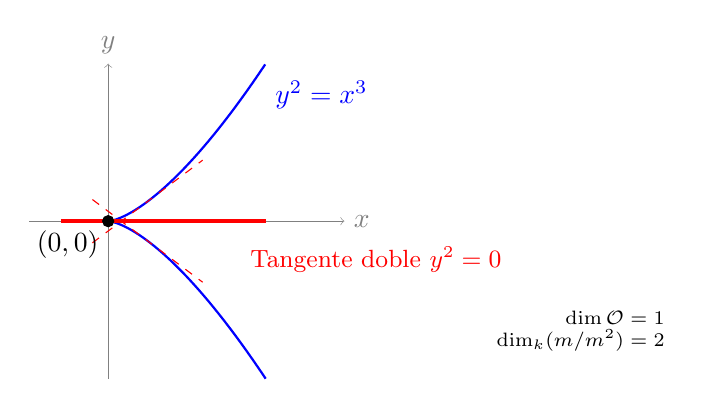
\begin{tikzpicture}[scale=2]
            % Ejes cartesianos
            \draw[->, help lines] (-0.5,0) -- (1.5,0) node[right] {$x$};
            \draw[->, help lines] (0,-1) -- (0,1) node[above] {$y$};
        
            % La cúbica cuspoidal y^2 = x^3 
            % Parametrización: x = t^2, y = t^3
            \draw[thick, blue, samples=100, domain=-1:1] plot ({\x*\x}, {\x*\x*\x});
            \node[blue, right] at (1,0.8) {$y^2=x^3$};
        
            % Rectas tangentes aproximándose (L1 y L2)
            % Tangente en t=0.5 (x=0.25, y=0.125) -> y - 0.125 = 0.75(x - 0.25)
            \draw[red, dashed, domain=-0.1:0.6] plot (\x, {0.75*\x - 0.0625});
            \draw[red, dashed, domain=-0.1:0.6] plot (\x, {-0.75*\x + 0.0625});
            
            % El límite: Espacio tangente doble (y=0)
            \draw[line width=1.5pt, red] (-0.3,0) -- (1,0);
            \node[red, below] at (1.7, -0.1) {\small Tangente doble $y^2=0$};
        
            % Punto singular en el origen
            \filldraw[black] (0,0) circle (1pt) node[anchor=north east] {$(0,0)$};
        
            % Notas aclaratorias
            \node[align=right, font=\scriptsize] at (3, -0.7) {
                $\dim \mathcal{O} = 1$ \\
                $\dim_k(\mathfrak{m}/\mathfrak{m}^2) = 2$ 
            };
        \end{tikzpicture}$$
    \end{ejem}
    ¿Es tangente en el origen?

    Consideramos la ecuación $x^3 + 0x^2 + 0x + y^2 = 0$. 
    ¿Cuál es su espacio tangente en el origen? 
    
    En este caso, la componente de menor grado (forma inicial) es $y^2 = 0$. Esto representa la recta $y=0$ contada 2 veces.
    
    Otro punto de vista: Graduados y Espacio Tangente
    
    Sea el morfismo de anillos dado por la proyección sobre $A$:
    $$\bt k{[x_i]} \rar{p \cdot} & k{[x_i]} \rar & A \rar & 0 \et$$
    Si consideramos el graduado asociado respecto al ideal maximal $\mathfrak{m}$, inducimos la sucesión:
    $$\bt G_{\m} k{[x_i]} \rar{p \cdot} & G_{\m} k{[x_i]} \rar & G_{\bar \m} A \rar & 0 \et$$
    
    Donde $G_{\mathfrak{m}} k[x_i] = k[x_i]$. Si $[p] \in \mathfrak{m}^r / \mathfrak{m}^{r+1}$, denotamos por $[p_r]$ su forma inicial de grado $r$. Luego, el graduado del anillo $A$ es:
    $$G_{\bar \m} A = \modulo{k{[x_i]}}{p \cdot k{[x_i]}} \simeq \text{Espacio Tangente}$$
    
    M\'as generalmente, si $A$ viene definido por varias ecuaciones $A = k[x_i]/(p_1, \dots, p_s)$, el espacio tangente es la intersección de los tangentes de cada $p_i = 0$. El conjunto de puntos $(\lambda_1, \dots, \lambda_n)$ del espacio tangente verifica:
    $$\{(\lambda_1, \dots, \lambda_n) \, / \, (p_1)_{r_1}(\lambda_1, \dots, \lambda_n) = 0, \dots, (p_s)_{r_s}(\lambda_1, \dots, \lambda_n) = 0\} $$
    Se prueba que el espacio tangente es, formalmente, $Spec(G_{\mathfrak{m}} A)$.
    \begin{defi}
        También se le llama \textbf{espacio tangente} al dual de $\modulo{\mathfrak{m}}{\mathfrak{m}^2}$. Es decir, $\left(\modulo{\mathfrak{m}}{\mathfrak{m}^2}\right)^*$ son los vectores tangentes.
    \end{defi} 

Sabemos que $\left(\modulo{\mathfrak{m}}{\mathfrak{m}^2}\right)^* = Der_k\left(A, \modulo{A}{\mathfrak{m}}\right)$, donde $\modulo{A}{\mathfrak{m}} \simeq k$. Dada una derivación $D$, $D: k[x_1, \dots, x_n] \longrightarrow k$ equivale a dar un elemento de $k^n$ (por la propiedad $Hom_{k-alg}$). Las derivaciones de $k[x_1, \dots, x_n]/(p_i)$ son aquellas derivaciones de $k[x_1, \dots, x_n]$ (elementos de $k^n$) que se anulan en el ideal generado por $p_i$.
\begin{ejem}
    $y^2 - x^3 = 0$

Una derivación $D$ es tangente si verifica:
$$\lambda \frac{\partial P}{\partial x}(0) + \mu \frac{\partial P}{\partial y}(0) = 0$$
En este caso, como las derivadas parciales en el origen son todas nulas ($0 + 0 = 0$), cualquier par $(\lambda, \mu)$ es una solución.

Si $(\lambda_1, \dots, \lambda_n) \in G_{\m} A$, entonces podemos definir la derivación como:
$$D = \sum \lambda_i \frac{\partial}{\partial x_i} \Big|_0$$
Lo cual constituye un vector tangente.

Formalmente, si consideramos el mapa $p: G_{\m} A \longrightarrow k$, donde $\lambda_i = p(x_i)$, esto nos permite identificar los puntos del esquema tangente con los vectores del espacio dual.
\end{ejem}
    
    
\cleardoublepage

 
\chapter{Morfismos finitos y dependencia entera}\justifying 

Sea $k$ un cuerpo y $k \to A$ una $k$-álgebra. Hay un morfismo asociado $Spec\, A \longrightarrow Spec\,  k = \{ * \}$. 
\textquestiondown Cuándo es $Spec A$ finito? Cuando $A$ es una $k$-álgebra finita (por ejemplo, tiene dimensión finita como espacio vectorial). En este caso, la topología es la discreta (ningún primo contiene a otro; todos son maximales).
\section{Morfismos finitos}
\begin{defi}
    Un morfismo de anillos $f: A \to B$ se dice \textbf{finito} cuando $B$ es un $A$-módulo finitamente generado, es decir, $B$ es una $A$-\'algebra finita. 
\end{defi}
Dado un ideal primo $\p \subseteq A$, \textquestiondown cómo es la fibra $(f^*)^{-1}(\p)$ bajo el morfismo inducido $f^*: Spec B \to Spec A$?.

\noindent \textbf{Fibra de $\mathfrak{p}$:} Como $B$ es un $A$-módulo, consideramos la localización y cociente $B_{\p} / \p B_{\p}$. Resulta que:
$$Spec(B_{\p} / \p B_{\p}) \hookrightarrow Spec B$$
y la imagen es el conjunto $\{\bar \p \in Spec B / f^{-1}(\bar \p) = \mathfrak{p}\}$. Por lo tanto, la fibra se identifica como:
$$(f^*)^{-1}(\mathfrak{p}) \simeq Spec(B_{\p} / \p B_{\p}) \cong Spec(B \underset{A}{\otimes}\kk (\mathfrak{p})) \text{}$$
Donde $\kk (\mathfrak{p})$ es el cuerpo residual de $A$ en $\mathfrak{p}$.

Hay un diagrama conmutativo de cambios de base:
\begin{center}
\begin{tikzcd}
Spec(B \underset{A}{\otimes}\kk (\mathfrak{p})) \arrow[r] \arrow[d] & Spec B \arrow[d, "f^*"] \\[5mm]
Spec(\kk (\mathfrak{p})) \arrow[r, hook] & Spec A
\end{tikzcd}
\end{center}

Como el cambio de base mantiene la finitud, si $A \to B$ es finito, entonces $\kk (\p) \to B \underset{A}{\otimes}\kk (\p)$ también es finito. Al ser $B \underset{A}{\otimes}\kk (\mathfrak{p})$ una $\kk(\mathfrak{p})$-álgebra finita, su espectro (la fibra) es un conjunto discreto y finito.
\begin{defi}
    Sea $f: A \to B$ un morfismo y $B$ una $A$-álgebra. Un elemento $b \in B$ es \textbf{entero sobre $A$} cuando $b$ verifica una ecuación polinómica en $A[x]$ mónico, es decir, 
    $$\exists \,  p(x) \in A[x] \text{ mónico tal que } p(b) = 0 $$
\end{defi}
\begin{propis}
\begin{enumerate}
    \item Si $f: A \to B$ es finito, entonces sus fibras son finitas y discretas. (demostraci\'on arriba)
    \item Si $f$ es inyectivo, entonces $f^* : Spec\, B \longrightarrow Spec \, A$ es epiyectivo.
    \begin{dem}
        Para cada primo $\p \subset A$, veamos que su fibra es no vac\'ia, pues $(f^*)^{-1} (\p) = Spec\, (B \underset{A}{\otimes}A_{\p} / \p A_\p)$, con $B_\p / \p B_\p = B \underset{A}{\otimes}A_{\p} / \p A_\p$, y debemos ver que $B_\p / \p B_\p \neq \emptyset$. $B_\p$ como $A$-m\'odulo, es $A_\p$-m\'odulo finito, pero $\p A_\p \subset A_\p $ es ideal maximal, as\'i pues, por Nakayama $B_\p / \p B_\p \neq 0 \iff B_\p \neq 0$, y como $A \hookrightarrow B$ es inyectivo, $A_\p \hookrightarrow B_\p$ es tambi\'en inyectivo, $0 \neq \p \subset A_\p$ existe en $B_\p$, luego $B_\p \neq 0$. 
    \end{dem}
    \item Si $f:A \to B$ es finito, $f^* : Spec\, B \longrightarrow Spec \, A$ es cerrada. Es decir, que $f^*((J_0)) = (f^{-1}(J))_0$.
    \begin{dem}
        Se tiene el diagrama
        $$\bt A \arrow{d} \rar{f} & B \arrow{d} \\ A/f^{-1}(J) \rar[hook]{\bar f} & B/J \et$$
        y entonces al pasar al espectro
        $$\bt  (f^{-1}(J))_0 \arrow[phantom]{r}{\subset} &[-13mm]  Spec\, A & \arrow{l}{f^*} Spec\, B &[-12mm] \arrow[phantom]{l}{\supset} (J_0)  \\[5mm]  
        & \arrow{ul}{\sim} Spec\, (A/f^{-1}(J)) \arrow[hook]{u} & \arrow{l}{\bar f^*} Spec\, (B/J) \arrow[hook]{u} \arrow{ur}{\sim} \et$$
        $\bar f$ es finito inyectivo, luego $\bar f^*$ es epiyectivo, y $f^*((J)_0) = (f^{-1} (J))_0$
    \end{dem}
    \begin{cor}
        Si $f^*$ es epiyectiva, sea $Z\subset Spec\, B$ un subconjunto cualquiera ${f^*}^{-1}(Z) \subset Spec\, B \Rightarrow Z = f^* ({f^*}^{-1}(Z)) = f^*(cerrado) = cerrado$
        y la topolog\'ia que tiene es la cociente, pudiendo entender $Spec\, A = Spec\, B / R_{f^*}$ por la relaci\'on de equivalencia dada por $f^*$.  
    \end{cor}
\end{enumerate}
\end{propis}
\begin{propis}
Dado $f: A \longrightarrow B$ un morfismo finito, entonces \vspace{-3mm}
\begin{enumerate}
    \item $\dim B \le \dim A$
    \begin{dem} Dada una cadena $\p_1 \subset \cdots \subset \p_n$ de primos de $B$, sus im\'agenes por $f^*$, veamos si se tiene la cadena estricta $f^{-1}(\p_1) \subsetneqq \cdots \subsetneqq f^{-1}(\p_n)$. Para el caso de dos, se tendr\'ia que son $\p\subsetneqq \p'$, entonces $f^{-1} (\p) \neq f^{-1}(\p')$.
    
    Supongamos no cierto, es decir, $f^{-1} (\p) = f^{-1}(\p') = \q \subset A$, de forma que $f^*(\p) = f^*(\p') = \q$, es decir, que ambos $\p\subsetneqq \p'$ est\'an en la fibra de $\q$, pero como las fibras de primos son discretas (maximales en las fibras), llegamos a contradicci\'on pues $\p = \p'$. 
    \end{dem}
    \item Si $f$ es inyectivo $\Rightarrow \dim B = \dim A$.
    \begin{dem}
        $f^*$ es cerrado y epiyectivo, se tiene la cadena de primos $\q_1 \subsetneqq \cdots \subsetneqq \q_n \subset A \hookrightarrow B$, entonces dada la cadena $\p_1 \subsetneqq \cdots \subsetneqq \p_n$ y cortarla con $A$, entonces para cada $i$, $\p_1 \overset{f^*}{\longrightarrow} \q_1$ y $A / \q_1 \hookrightarrow B / \p_1$ por el paso al cociente, y entonces $[\q_2] \subset A / \p_1$ tiene fibra en $B / \p_1$, que llamaremos $[\p_2] \subset B / \p_1$ por $f^*$.  
    \end{dem}
\end{enumerate}
\end{propis}
\begin{obs}
    No es lo mismo una \'algebra finita que de tipo finito.
\end{obs}
\section{Elementos enteros}
Sea $B$ una $A$-\'algebra, 
\begin{defi}
    Un \textbf{elemento} $b\in B$ se dice \textbf{entero} sobre $A$ cuando existe un polinomio $p(x) \in A[x]$ m\'onico ($p(x) = x^n + a_{n-1} x^{n-1} +\cdots + a_n$) tal que $p(b) = 0$. 
\end{defi}
\begin{prop} $b \in B$ es entero (sobre $A$) $\iff \, A[b] \subset B$ es $A$-\'algebra finita. Es decir, si $p(x) = \bar a_o x^{n} + \cdots +\bar a_n$, $p(b) = \bar a_o b^n + \cdots + \bar a_n \in B$ lo pensamos en $B$. 
\end{prop}
\begin{obs}
    Sea $p(x)$ m\'onico con $p(b)=0$, entonces $A[b]= (A[x]/p(x))/ I$ por el algoritmo de divisi\'on. Esto nos dice que $A[b]$ como $A$-m\'odulo es cociente de $A[x]/p(x)$, que es $A$-m\'odulo finito, con base $\{1, x, \ldots, x^{n-1}\}$, y por tanto $A[b]$ es finito.  
\end{obs}
\begin{dem}
    $\Leftarrow)$ $A[b]$ como $A$-m\'odulo es finito generado, y sean $\xi_1, \ldots, \xi_r$ un sistema de generadores, en particular
    $$\xi_j \cdot b = \sum a_{ij} \xi_i$$
    que nos da una matriz $(a_{ij})$, cuyo polinomio caracter\'istico $C(x) = |xId-M|$ cumple que $C(M)=0$. 

    Tenemos el diagrama conmutativo
    $$\bt A^n \rar{M} \arrow{d}{\pi} & A^n \arrow{d}{\pi} \\[5mm] A[b] \rar{ b\cdot} & A[b]\et \qquad  \bt 1_j \rar[mapsto] \arrow[mapsto]{d} & \sum a_{ij} 1_j \arrow[mapsto]{d} \\[5mm] \xi_j \rar[mapsto] & b \xi_j \coloneqq \sum a_{ij} \xi_j\et$$
    de forma que $\bb Z[x_{ij}] \subset \bb Q(x_{ij})$ con $C(\tilde M) = $polinomio con coeficientes en $\bb Z[x_{ij}]$, y es $C(\tilde M) = 0$, y $C(\tilde M) = Q(x,x_{ij})$ viene de una matriz $Q(\tilde M, x_{ij}) $ con coeficientes polinomios e $x_{ij}$ que es 0, por lo que al sustituir por $b$, sigue siendo 0.  Hemos demostrado que $C(b \cdot ) = 0 $ pero $b\cdot =h_b$, $C(h_b) = h_{c(b)} = 0 \iff C(b) = 0 $. 
\end{dem}
\begin{prop}
    Una \'algebra de tipo finito $A[\xi_1, \ldots, \xi_n]$ es finita $\iff$ todo elemento es entero, en particular $\xi_1, \ldots, \xi_n$ son enteros.
\end{prop}
\begin{dem}
    $\Rightarrow)$ $A[\xi_1, \ldots, \xi_n]$ es finita implica que $\xi_n$ es entero sobre $A$, usando la misma demostraci\'on que en la proposici\'on anterior, $\bar \xi_1, \ldots \bar \xi_r$ generadores de $A[\xi_1, \ldots, \xi_n]$, $\xi_ \cdot \bar \xi_j = \sum a_{ij} \bar \xi_i$. 

    $\Leftarrow)$ Los morfismos $A[\xi_1] \hookrightarrow A[\xi_1,\xi_2] \hookrightarrow \cdots \longrightarrow A[x_1, \ldots, \xi_n]$ cada morfismo es finito sobre el anterior, y por tanto sobre el primero (\textcolor{red}{ejercicio} si $A \to B \to C$ son finitos, entonces $A \to C$ es finito). 
\end{dem}
\begin{lem}
    Si $b_1, \ldots, b_r \in B$ son enteros, entonces $p(b_1, \ldots, b_r)$ es entero por cualquier $p(x_1, \ldots, x_r) \in A[x_1, \ldots, x_r] $
\end{lem}
\begin{dem}
    $A \hookrightarrow A[b_1, \ldots, b_r] = B$ es finito porque añadir $b_i$ es finito, por ser $b_i$ enteros, y as\'i.
\end{dem}
\begin{obs}
    Hemos visto pues que los enteros de $B$ sobre $A$ es una sub\'algebra de $B$, que llamaremos el cierre entero de $A$ en $B$, y se denota por $\bar A$, y se tiene $A \to \bar A \subset B$, como $B$ no tiene elementos enteros sobre $\bar A$ (salvo los de $\bar A$, pues si un elemento $b \in B$ es entero sobre $\bar A$, verifica una ecuaci\'on $x^n + \bar a_1 x^{n-1} +\cdots +\bar a_n$, con $\bar a_i \in \bar A$, se tendr\'ia que $A[\bar a_1, \ldots, \bar a_n]\subset  A[\bar a_1, \ldots, \bar a_n][b]$ es finito, y $A \to A[\bar a_1, \ldots, \bar a_n]$ tambi\'en es finito, en particular $A\to A[\bar a_1, \ldots, \bar a_n,b]$ es finito, $b$ es entero sobre $A$ y por tanto $b\in \bar A$). 
\end{obs}
\begin{ejem}
    Sea $A$ \'integro, $\Sigma=A_o, \, A \subset \Sigma \hookrightarrow k$, y $\bb Z \subset \bb Q\hookrightarrow k \supset \bar{ \bb Z}$ es libre y finito generado como $\bb Z$-m\'odulo, es decir, $\bar {\bb Z} = [\alpha_1, \ldots, \alpha_r]$.
\end{ejem}
\begin{custom}[Recordatorio dfu]
    Sea $A$ un dominio de factorizaci\'on \'unica (todo $a\in A$, $a=u p_1^{n_1} \cdots p_r^{n_r}$ con $p_i$ irreducible (es decir, si $p=q_1\cdot q_2$, entonces $q_1 = \bar u \cdot p$ \'o $q_2 = u' \cdot p$), y es \'unica (si $a = u' q_1^{m_1} \cdots q_{r'}^{m_{r'}}$, salvo reordenaciones, $p_i=q_i\cdot u_i$ salvo unidades, $r=r'$ y $n_i = m_i$). Adem\'as, un elemento $p$ es irreducible $\iff$ $p$ es primo ($pA$ es ideal primo).  
\end{custom}
\begin{ejem}
    $\bb Z,\, k[x]$ son dominios de factorizaci\'on \'unica. Adem\'as el Lema de Gauss asegura que si $A$ es dfu, entonces $A[x]$ es dfu. Por ejemplo, $k[x_1,\ldots, x_n],\bb Z[x_1,\ldots, x_n]$ son dfus aunque ya no son de ideales principales.
\end{ejem}
\begin{defi}
    Sea $A$ \'integro, se dice \textbf{\'integramente cerrado} en su cuerpo de fracciones $A \subset \Sigma$ si $\bar A = A$ (es decir, no hay fracciones que sean enteras). 
\end{defi}\begin{lem}
    No hay fracciones que sean enteras, en su cuerpo de fracciones no hay enteros. 
\end{lem}
\begin{dem}
    Sea $\frac{a}{b} \in \Sigma$ irreducible,
    $$\left(\frac{a}{b} \right)^{n} + a_1 \left(\frac{a}{b} \right)^{n-1} + \cdots + a_n = 0 $$
    $$a^n  = -a_1 b a^{n-1} + \cdots - b^n a_n$$
    entonces, si $p$ divide a $b$, divide a $a^n \Rightarrow $ divide a $a$, ser\'ia un primo com\'un de $a$ y $b$, llegando a contradicc\'on (supusimos que la fracci\'on es irreducible), entonces $b$ es un unidad. 

    Entonces, en un dominio de factorizaci\'on \'unica, son \'integros, cerrados.
\end{dem}
\begin{lem}
    [de normalizaci\'on de Noether] Supongamos que $A = k[\xi_1, \ldots, \xi_n]$ (el anillo de funciones de una variedad algebraica). Existe un morfismo finito 
    $$\bt k[x_1, \ldots, x_d] \rar & A \et $$
    es decir, un morfismo finito $Spec \, A \longrightarrow \bb A_d$. 
\end{lem}
\begin{dem}
    $$\bt k[\xi_1', \ldots, \xi'_{n-1}] \rar[hook]{finito} & k[\xi_1', \ldots, \xi'_{n-1}, \xi'_n] \\ k[x_1, \ldots, x_d] \arrow{ru} \arrow[hook]{u}{finito} \et$$
    y entonces si $\xi_1, \ldots, \xi_n$ son algebraicamente independientes, entonces $k[\xi_1, \ldots, \xi_{n}] \simeq k[x_1, \ldots, x_n]$. Vamos a decir que el monomio $\xi_1^{m_1} \cdots \xi_r^{m_r}$  es mayor que otro cuando $(m_1, \ldots, m_r) \ge (m_1' , \ldots, m_r')$ en orden lexicogr\'afico, $m_1 \geq m_1'$ \'o si $m_1 = m_1'$, entonces $m_2 \ge m_2'$ \'o si $m_2 = m_2'$, ...

    Sea $p(\xi_1, \ldots, \xi_n) = \xi_1^{m_1} \cdots \xi_n^{m_n}  + \cdots = 0$, hacemos el cambio de variable $\xi_1'=\xi_1-\xi_n^{d_1}, \, \xi_2'=\xi_2-\xi_n^{d_2}, \ldots, \xi_{n-1}'=\xi_n-\xi_n^{d_n}, \xi_n' = \xi_n$, de forma que $d_1 \gg  d_2 \gg  d_3 \gg  \cdots \gg  d_n$.  $A = k[\xi_1', \ldots, \xi_n']$, entonces $p(\xi_1, \ldots, \xi_n)  = \bar p(\xi_1', \ldots, \xi_n') = q(\xi_1', \ldots, \xi_{n-1}'){\xi'}_n^r + \cdots  = 0$ y demostrando que $q=1$, vemos que $k[\xi_1', \ldots, \xi'_{n-1}] \longleftarrow k[\xi_1', \ldots, \xi'_{n-1}, \xi'_n] $ es finito. 
    $$\xi_1^{r_1} \cdots \xi_n^{r_n} \longmapsto (\xi_1' + \xi_n^{d_1})^{r_1} \cdots (\xi_{n-1}' + \xi_{n-1}^{d_1}) \xi_n$$
    de forma que el grado es $r_1d_1+r_2d_2 + \cdots + r_{n-1} d_{n-1} + r_n$ y como $(\xi_1' + \xi_n^{d_1})^{r_1} \cdots (\xi_{n-1}' + \xi_{n-1}^{d_1})$ es m\'onico por serlo cada uno de ellos, por lo que es m\'onico sobre $\xi_n$ y $\bar p(\xi_1',\ldots, \xi_{n-1}', x)$ es m\'onico asegurando la finitud del morfismo. 
\end{dem}

Tenemos que $k[x_1, \ldots, x_r] \hookrightarrow k[\xi_1, \ldots, \xi_n]$ es un morfismo finito
\begin{obs}
    $\dim(k[x_1, \ldots, x_n] ) = n$, que lo hemos visto en el origen, localmente, pero en general se usa con el polinomio de Hilbert y el graduado. $ 0 \subset (x_1) \subset (x_1,x_2) \subset \cdots \subset (x_1, \ldots, x_n)$ es una cadena de ideales primos de longitud $n$, entonces $\dim(k[x_1, \ldots, x_n] ) \ge n$. Por inducci\'on sobre $n$, vamos a ver que $\dim(k[x_1, \ldots, x_n] ) \geq n\dim(k[x_1, \ldots, x_n] ) \le n$. Sea $0 \subset \p_1 \subset \cdots \subset \p_r$, vamos a ver que $r \le n$. Escojamos $0\neq p\in \p_1$, en $k[x_1,\ldots, x_n]/p $, se tiene la cadena $\bar \p_1 \subset \bar \p_2 \subset \cdots \subset \bar \p_r$ con $\bar \p_i = \p_i / p k[x_1, \ldots, x_n]$ pero $k[x_1,\ldots, x_n]/p =k[\xi_1, \ldots, \xi_n]$ es de tipo finito, y por el mismo argumento que en la demostraci\'on del Lema de Noether, se puede hacer un cambio de variable, de forma que $k[\xi_1, \ldots, \xi_n] = k[\xi'_1, \ldots, \xi'_n][\xi_n] \supset k[\xi'_1, \ldots, \xi'_{n-1}] $ es finita, y hay un morfismo finito de $k[y_1, \ldots, y_m] \subset k[\xi'_1, \ldots, \xi'_{n-1}]$, de forma que $\dim(k[y_1, \ldots, y_m]) = m \le n-1 $, luego $\dim(k[x_1,\ldots, x_n]/p) = m \le n-1$ y por tanto
    $$r-1 = \ell(\bar \p_1 \subset \cdots \subset \bar \p_r) \le \dim k[x_1,\ldots, x_n]/p  = m \le n-1$$
    $$\Rightarrow r \le n$$
\end{obs}
\begin{cor}[Teorema de los ceros de Hilbert]
    $k \hookrightarrow k[\xi_1, \ldots, \xi_n]/\m$ es finita.
\end{cor}\begin{dem}
    $k \hookrightarrow k[\xi_1, \ldots, \xi_n]/\m = k[\bar \xi_1, \ldots, \bar \xi_n]$ es cuerpo, y por el Lema de Noether hay una inmersi\'on finita $k[x_1,\ldots, x_s] \hookrightarrow k[\bar \xi_1, \ldots, \bar \xi_n]$, pero $k[\bar \xi_1, \ldots, \bar \xi_n]$ es de dimensi\'on 0, pero como la inyecci\'on es finita, las dimensiones coinciden luego $\dim(k[x_1,\ldots, x_s] ) = s = 0$, es decir, $k[x_1,\ldots, x_s] = k$. 
\end{dem}
\begin{prop}
    $Rad(k[\xi_1, \ldots, \xi_n]) = Rad_{J}k[\xi_1, \ldots, \xi_n]$ siendo el radical de Jacobson $\bigcap $Maximales, y en general $\bigcap \p \subseteq \bigcap \m$, hay que demostrar que $\supseteq$. 
\end{prop}
\begin{dem}
    Sea $f\in \bigcap \m, f\nin \bigcap \p$, $Spec \, (k[\xi_1, \ldots, \xi_n]_f) \subset k[\xi_1, \ldots, \xi_n][\frac{1}{f}]$ pero $Spec(k[\xi_1, \ldots, \xi_n]_f) = Spec k[\xi_1, \ldots, \xi_n] -(f)_0 \neq \emptyset$. As\'i, 
    $$\bt k[\xi_1, \ldots, \xi_n]\arrow[bend left=8mm]{rr}{\pi} \rar & k[\xi_1, \ldots, \xi_n]_f \rar & k[\xi_1, \ldots, \xi_n]_f/\m \\[-5mm] f \rarmaps & \text{invertible} \rarmaps & \text{invertible} \neq 0 \et$$ de forma que si $\p = \ker \pi$, $k[\xi_1, \ldots, \xi_n]/\p \hookrightarrow k[\xi_1, \ldots, \xi_n]/\bar \m$ es un cuerpo, y de tipo finito, luego es una extensi\'on finita de $k$, con $k \hookrightarrow k[\xi_1, \ldots, \xi_n]/\p$, concluyendo que $k[\xi_1, \ldots, \xi_n]/\p$ es $k$-\'algebra finita \'integra, por lo que es cuerpo y $\p$ es maximal, de forma que $f$ es invertible en $k[\xi_1, \ldots, \xi_n]_f$, luego $f\neq 0$ y como $f \nin \bar \m$, $f\nin \p$, hemos encontrado un maximal que no contiene a $f$. 
\end{dem}
\begin{obs}
    $\frac{p(\xi_1, \ldots, \xi_n)}{f^r}= \frac{1}{f^r} p(\xi_1, \ldots, \xi_n) \in k[\xi_1, \ldots, \xi_n][\frac{1}{f}] $
\end{obs}
\begin{obs}
    Dado $p(x_1, \ldots, x_n)$ con $p(\alpha_1, \ldots, \alpha_n) = 0$ para todo soluci\'on del sistema, entonces $p^m = \sum_{i=1}^n \lambda_i (x_1, \ldots, x_n) p_i$.  
\end{obs}
\begin{prop}
    Sea $A$ un anillo \'integro local de ideales principales, entonces $A$ es normal ($A \subset \Sigma = A_o$), es decir, $\bar A = $ cierre entero de $A$ en $\Sigma=$ los elementos de $\Sigma$ enteros sobre $A = A$. 
\end{prop}
\begin{dem}
    Sea $\frac{a}{b} \in \Sigma$ entera sobre $A$, $a= u \cdot p_1^{n_1} \cdots p_r^{n_r}, \, b = \bar u \cdot q_1^{n_1} \cdots q_s^{n_s}$, podemos suponer que no tienen primos comunes, de forma que $\frac{a}{b}$ es irreducible y $\nin A$, siendo $b$ no invertible, luego $b$ es divisible por un primo $q$ y $a$ no es divisible por $q$.  
    $$\left(\frac{a}{b} \right)^{n} + a_1 \left(\frac{a}{b} \right)^{n-1} + \cdots + a_n = 0 $$
    $$a^n  = -a_1 b a^{n-1} + \cdots - b^n a_n$$
    y si $q$ divide a $ -a_1 b a^{n-1} + \cdots - b^n a_n$, $q$ divide a $a^n$ y entonces $q$ divide a $a$. 
\end{dem}
\section{Anillos de valoraci\'on}
\begin{defi} Sea $A$ \'integro y $\Sigma = A_o$ su cuerpo de fracciones, una \textbf{valoraci\'on} es un morfismo
    $\nu : \Sigma^{\times} \longrightarrow G$ siendo $G$ un grupo abeliano totalmente ordenado, es decir, para todo $g_1,g_2\in G \Rightarrow g_1 \le g_2 \text{ \'o } g_2\le g_1$, y si $g_1\le g_2, g\in G \Rightarrow g_1 + g \le g_2 + g$. Entonces $\nu$ es morfismo de grupos ($\nu(fh) = \nu (f) + \nu(h)$) y $\nu(f+h) = \min(\nu(f), \nu(h))$. 
\end{defi}
\begin{ejem}
    Si $A=k[x_1, \ldots, x_n]$, $\m=\m_o$ $\nu(p(x_1, \ldots, x_n)) = h$ co $p(x_1, \ldots, x_n) \in \m^h - \m^{h+1}$ entonces $\nu: k(x_1, \ldots, x_n)^{\times} \longrightarrow \bb Z$ y $\nu\left(\frac{p}{q}\right) = \nu(p)-\nu(q)$, y es lo que se llama la valoraci\'on $\m$-\'adica, que es el rango de un polinomio, el menor de sus grados, que es cu\'antas veces se anula en el origen. 
\end{ejem}
\begin{ejem}
    Si $\mc O$ es un anillo local noetheriano, $\m \subset \mc O$ el maximal, entonces
    $$\nu_{\m} (f) = h \iff f\in \m^h - \m^{h+1}$$
    $$\nu_{\m}\left(\frac{f}{g} \right) = \nu_\m (f) - \nu_\m(g)$$
\end{ejem}

\begin{defi}
    Decimos que un \textbf{anillo} es \textbf{de valoraci\'on} cuando para cada $f \in \Sigma$ se verifica que $f\in A$ \'o $f^{-1} \in A$. 
\end{defi}
\begin{ejem}
    Sea $\Sigma$ un cuerpo y $\nu: \Sigma^{\times} \longrightarrow G$ una valoraci\'on, consideramos los elementos $A = \{ f \in \Sigma \,/\, \nu(f) \ge 0\}=\mc O_{\nu}$, y se cumple que $A$ es un anillo local y de valoraci\'on, y $\m = \{f\in \Sigma \, / \, \nu(f) > 0\}$. Se define $\nu(0)=\infty$ tal que $g+ \infty = \infty, \, \infty  + \infty = \infty$. Aunque se convierte en semigrupo.
\end{ejem}
\begin{teo}
    $\mc O_{\nu}$ es anillo local de valoraci\'on.
\end{teo}
\begin{dem}
    Es de valoraci\'on, pues dada $f\in \Sigma^{\times}$, entonces $f\in \mc O_{\nu}$ \'o $f^{-1}\in \mc O_{\nu}$ ya que como $\nu(f^{-1}) = -\nu(f)$, y $\nu(f)$ es totalmente ordenado, luego $\nu(f) \ge 0$ \'o $\nu(f) \le 0$. En el primer caso $f\in \mc O_{\nu}$, y en el segundo caso, como $\nu(f^{-1}) = - \nu(f) \ge 0$, y por tanto $f^{-1} \in \mc O_{\nu}$.

    Es local, es decir, $\m \subset\mc O_{\nu}$ es ideal maximal. Por la desigualdad, es ideal, si $\nu(f) \ge 0, \nu(h) \ge 0$, $\nu(f+h) \ge \min(\nu(f)(>0) , \nu(h)(>0) ) > 0 $, es decir, si $f, h\in \m \Rightarrow f+h \in \m$. Si $f\in \m, h \in \mc O_{\nu}$, 
    $$\nu(f\cdot h) = \nu(f) (>0) + \nu(h)(\ge 0) > 0 $$
    
    Para ver que es maximal, veamos que todo elemento que no pertenece a \'el es invertible. Es decir, si $a\in \mc O - \m\Rightarrow a $ es invertible. \textcolor{red}{Ejercicio}. $a\in \mc O - \m$, $\nu(a) \ge 0, \, \nu(a) \not> 0 \Rightarrow \nu(a)=0, \, \nu(a^{-1}) = -\nu(a) = 0 \Rightarrow a^{-1} \in \mc O$. 
\end{dem}

Todo anillo $\mc O$ de valoraci\'on, define una valoraci\'on $\Sigma^{\times} \overset{\nu}{\longrightarrow} \Sigma^{\times} / \mc O^{\times}$ es una valoraci\'on con $[f] \le [h]$ cuando $\frac{h}{f} \in \mc O^{\times}$. $f\ge h, \, h\in \Sigma^{\times}, fh'\ge hh'$. $\frac{fh'}{hh'} = \frac{f}{h} \in \mc O^{\times}$. Es decir, $f \ge h$ \'o $h\ge f$, $\frac{f}{h} \in \mc O$ \'o $\frac{h}{f}\in \mc O$. Entonces $\mc O_{\nu} = \{f\in \Sigma\, / \, \nu(f) \ge 0 = \nu(1)\}$ pues $\nu(f) \ge \nu(1), f\ge 1 \Rightarrow \frac{f}{1} \in \mc O$, luego $\mc O_{\nu} = \mc O$.

\begin{prop}
    Una valoraci\'on define un anillo de valoraci\'on, y viceversa.
\end{prop}
\begin{dem} 
Dado $\nu$, $\mc O_{\nu}$ es de valoraci\'on, con $f\in \Sigma \Rightarrow \nu(f) \ge 0$ \'o $\nu(f) \le 0 \Rightarrow f\in \mc O_{\nu}$ \'o $f^{-1}\in \mc O_{\nu}$ y como $\Sigma \in (\mc O_{\nu})_o$, $f\in \Sigma \Rightarrow f\in\mc O_{\nu}\subset (\mc O_{\nu})_o$ \'o $f^{-1} \in \mc O_{\nu} \subset (\mc O_{\nu})_o \Rightarrow f\in (\mc O_{\nu})_o$. 

Dado $\mc O$ anillo de valoraci\'on, se tiene el grupo $G=\modulo{\Sigma^{\times}}{\mc O^{\times}}$, que define la valoraci\'on  $\Sigma^{\times} \overset{\nu}{\longrightarrow} \Sigma^{\times} / \mc O^{\times}$ y falta que est\'e totalmente ordenado. Se tiene que $f \le h$ cuando $\frac{h}{f} \in \mc O^{\times}$, y para que se cumpla la propiedad antisim\'etrica, $f\le h \le f \iff \frac{h}{f}$ y $\frac{f}{h} \in \mc O \iff \frac{h}{f} \in \mc O^{\times}$, que como clases de equivalencia es 
$$\bar f \le \bar h \le \bar f \iff \left( \overline{\frac{h}{f}} \right)=1 \iff \bar h = \bar f$$
es decir, $\le$ es un orden parcial. Para que sea total falta que est\'e definido para todo elemento. $f, h\in \Sigma \Rightarrow f\le h$ \'o $h \le f$, $\frac{f}{h}$ \'o $\frac{h}{f} \in \mc O$. Falta ver que $\nu(f+h) \ge \min(\nu(f),\nu(h))$, es decir, que $\nu(f+h) \ge \nu(f)$ \'o $\nu(h)$.  $f \le h$ \'o $h \le f$. Supongamos $f \le h$, entonces $\frac{h}{f} \in \mc O$, luego 
$$f+h = f\left(1+\frac{h}{f}\right) \Rightarrow \frac{f+h}{h} = 1+\frac{h}{f} \in \mc O \Rightarrow f+h \ge f$$ 
\end{dem}
\begin{defi}
    Decimos que una \textbf{valoraci\'on} es \textbf{discreta} cuando $G \simeq \bb Z$ pensando $G$ como $\Im \nu$. 
\end{defi}
\begin{ejem}
    Sea $A$ de ideales principales con $A_\p$, se tiene la valoraci\'on $\Sigma^{\times} \overset{\nu}{\longrightarrow} \bb Z$, con
    $$\frac{f}{h} = \frac{mp^n}{np^s} = \frac{m}{n} p^{r-s} \longmapsto r-s$$
    es decir, en $k[x]$, $\frac{p(x)}{q(x)} \longmapsto$ multiplicidad de $\frac{p(x)}{q(x)}$ en $x=\alpha$. El anillo de valoraci\'on es $\mc O_{\nu} = A_\p$ por la f\'ormula, pues las fracciones de valor positivo son las que tienen el denominador no divisible por $p\in \p$. 
\end{ejem}
\begin{defi}
   Sea $\mc O \supset \m$ local, $\mc O \longrightarrow B$ es \textbf{dominante} cuando existe $\m ' \subset B$ con $\m' \cap \mc O = \m$. Como $\mc O \subset \Sigma$ y $\mc O'\subset \Sigma$, entonces $\mc O \le \mc O'$ domina si $\mc O \subset \mc O'$. 
\end{defi}
\begin{teo}
    Un anillo local es de valoraci\'on $\iff$ es maximal en $\Sigma$ con el orden de dominaci\'on. Esto es, si $\mc V \subset \Sigma$ de valoraci\'on, $\mc V \le B \subset \Sigma$, siendo $\mc V$ anillos locales $\Rightarrow B = \mc V$. Rec\'iprocamente, si $\mc V \subset \mc V_o$ es maximal $\Rightarrow \mc V$ es de valoraci\'on.
\end{teo}
\begin{dem}
    $\Rightarrow)$ Supongamos $\mc O$ de valoraci\'on, entonces demostraremos que si $\mc O \le \mc O' \Rightarrow \mc O' = \mc O$. 

    Supogamos $b\in \mc O, b\nin \mc O$. Entonces $b^{-1} \in \mc O \Rightarrow b^{-1} \in \m$. Entonces $b^{-1} \in \m \mc O '$ y $b\in \mc O' \Rightarrow \m \mc O' = \mc O'$, pero al estar dominado se tiene que $\m' \cap \mc O = \m \Rightarrow \m'\supset \m$, por lo que $\m \mc O ' =\mc O' \subset \m' \, !!$

    $\Leftarrow)$ Supogamos ahora que $\mc O$ es maximal. Sea $f\in \Sigma \, / \, f\nin \mc O$. $\mc O \hookrightarrow \mc O[f]$ es un anillo m\'as grande, y $(\mc O[f])_{\p'}$ ya es local de forma que $\mc O \subsetneqq (\mc O[f])_{\m'}$, es decir, domina, luego $\m$ no tiene fibra en $\mc O[f]$. Por lo que $Spec(\mc O' / \m \mc O') = \emptyset\Rightarrow \m \mc O[f] = \mc O[f]$ y entonces $1=a_of^n + a_1 f^{n-1} + \cdots + a_n$, $a_1, \ldots, a_n \in \m$, y por tanto, 
    $$f^{-n} -a_n f^{-n} - a_{n-1} f^{-(n-1)} - \cdots - a_o = (1-a_n) f^{-n} - a_{n-1} f^{-(n+1)} - \cdots - a_o = 0 $$
    y $1-a_n$ es invertible $(1\nin \m)$, diviendo por \'el, 
    $$f^{-n} - \frac{a_n}{1-a_n} f^{-(n-1)} - \cdots - \frac{a_o}{1-a_n} = 0 $$
    luego $f^{-1}$ es entero sobre $\mc O$, es decir, el morfismo $\mc O \hookrightarrow \mc O[f^{-1}]$ es finito, $\m'$ tiene fibra y al localizar, $\mc O \hookrightarrow \mc O[f^{-1}]_{\m'}$ es dominante, y $\mc O[f^{-1}] = \mc O $ con lo que $f^{-1} \in \mc O$. 
\end{dem}
\begin{teo}
    Sea $\mc O$ anillo local \'integro, 
    \begin{enumerate}[1)]
        \item $\mc O$ es de valoraci\'on discreta.
        \item $\mc O$ es de ideales principales ($\equiv \, \m$ es principal).
        \item $\mc O$ noetheriano de $\dim 1$ y normal.
        \item $\mc O$ noetheriano de $\dim 1$ y regular.
    \end{enumerate}
\end{teo}
\begin{dem}
    1) $\Rightarrow$ 2) $\mc O$ es de valoraci\'on discreta, la valoraci\'on es $\nu(\frac{f}{g}) = \nu (f) - \nu (g) $ siendo $\nu(f) = n$ con $f\in \m^n, \, f\nin \m^{n+1}$. Veamos que $\m = t\cdot \mc O$. $\mc O$ es de valoraci\'on discreta, entonces consideremos un $f \in \m$, con $n$ la m\'inima tal que $\m^n \subset f\mc O$, y como $f\in \m^n, \, f\nin \m^{n+1}$, consideramos $h \in \m^{n+1}$, $h \nin f \mc O$. Entonces $x=\frac{h}{f} \nin \mc O, \, x\m  = \frac{h}{f} \m \subset \frac{1}{f}h\m \subset \frac{1}{f} \m^{n-1} \m = \frac{1}{f} \m^n \subset \mc O$. 

    As\'i, $x \cdot \m \subset \mc O$ es un ideal, luego o bien es $x\m =\mc O$, $\m = \frac{1}{x} \mc O$ por tanto es principal, o bien $x\m \subset \m$ y $x\cdot $ es endomorfismo, y como es noetheriano (de valoraci\'on discreta) finito generado, tiene anulador y es un polinomio m\'onico, entonces $x$ es entero sobre $\mc O$, es decir, $\mc O \longrightarrow \mc O[x]$ es finito, en el espectro es epiyectivo, es decir, el maximal tienen fibra, y como $\mc O$ es de valoraci\'on, $\mc O \hookrightarrow \mc O[x]_{\m'}$ es finito y dominante, $\mc O = \mc O[x] \Rightarrow x\in \mc O$, llegando a contradicci\'on. 
    
    2) $\Rightarrow$ 1) Pr\'oxima proposoci\'on. 
    
    2) $\Rightarrow$ 3) 
    
    3) $\Rightarrow$ 2)
\end{dem}

\begin{prop}
    Si $\mc O$ es local de ideales principales $\Rightarrow $ es de valoraci\'on discreta ($2) \Rightarrow 1)$).
\end{prop}
\begin{dem}
    $\m = t\mc O, \, f\in \mc O \Rightarrow f=ut^n$ con $u$ invertible, 
    $$\frac{f}{g} = \frac{ut^n}{\bar u t^m} = u t^r \quad r \in \bb Z; \, \nu\left(\frac{f}{g}\right) = r$$
    es una valoraci\'on y discreta.
\end{dem}
\begin{teo}
    Sea $\mc O$ local e \'integro. Las siguientes condiciones son  equivalentes:
    \begin{enumerate}[1)]
        \item $\mc O$ es de valoraci\'on discreta.
        \item $\mc O$ es de ideales principales ($\equiv \, \m$ es principal).
        \item $\mc O$ es de valoraci\'on y noetheriano.
    \end{enumerate}
\end{teo}
\begin{dem}
    2) $\Rightarrow$ 3) Por lo anterior.

    3) $\Rightarrow$ 2) Sea $I\subset \mc O$ un ideal, $\mc O$ es noetheriano, entonces entre sus generadores consideremos el de menor valor, como $I = (\xi_1, \ldots, \xi_n)$, consideramos el m\'inimo $\nu(\xi_1)=\min (\nu(\xi_2), \ldots, \nu(\xi_n))$. Si $\xi \in I$; $\nu(\xi_1) \le \nu(\xi) \Rightarrow \nu \left( \frac{\xi}{\xi_1} \right) \ge 0, \, \frac{\xi}{\xi_1} \in \mc O$. Entonces $\xi = \xi_1 \cdot \frac{\xi}{\xi_1} \Rightarrow \xi \in \xi_1 \mc O$, y como $\xi = a_1\xi_1 + \cdots + a_n \xi_n$, $\nu(\xi) \ge \min(\nu(a_i\xi_i)) = \min(\nu(a_i)+ \nu(\xi_i)) \ge \min(\nu(\xi_i)) = \nu(\xi)$.

    1) $\Rightarrow$ 2) Sea $I \subset \mc O$ ideal, como $\nu(I) \subset \bb N$, el generador es de valor m\'inimo, $\xi_1 \in I \, / \, \nu(\xi_1)$ es m\'inimo en $I$. Por lo que el ideal es pricipal
\end{dem}
\section{Normalidad}
\begin{defi}
    Sea $A$ \'integro, se dice \textbf{normal} cuando el cierre entero de $A$, $\bar A$, en $A_o = \Sigma$ es $A$. Es decir, \'integramente cerrado en su cuerpo de fracciones.
\end{defi}
\begin{prop}
    Si $\mc O$ es local noetheriano de $\dim 1$, regular (no singular) $\iff \, \m = t\mc O$ es principal $\iff \, \mc O$ es de ideales principales.
\end{prop}
\begin{dem}
    Sea $0 \neq I \subset \m \subset \mc O$, como $\mc O$ es de $\dim 1$, $\mc O / I$ es de $\dim 0$ noetheriano y local, luego $Spec \, \mc O / I = \{\bar \m\} \Rightarrow \rad \mc O / I =\bar \m \Rightarrow \bar \m =0$, por lo que $\m^n \subset I \subset \m$. Sea $I\subset \m^r$, la maxima potencia que contiene a $I$, entonces, $I \longrightarrow \m^r / \m^{r+1} \simeq t^r \mc O / t^{r+1} \mc O \simeq \mc O / t^r \mc O = \mc O / \m = k$ de forma que $\dim \m^r / \m^{r+1} = 1$ como $k$-e.v. y existe $\xi \in I$ tal que $\xi \in \m^r$ es base en $\m^r / \m^{r+1} = \m^r / \m\cdot \m^r$. Entonces $\xi$, por Nakayama, es generador de $\m^r$, luego $\xi \mc O = \m^r$. Se tiene que 
    $$\m^r \supset I \supset \xi \mc O = \m^r \Rightarrow \m^r = I$$
\end{dem}
\begin{lem}
    Todo anillo $\mc V$ de valoraci\'on es normal.
\end{lem}
\begin{dem}
    Sea $f\in \mc V_o = \Sigma$ y entero sobre $\mc V$. Sea $\mc V \hookrightarrow \mc V[f]$, es finito, que en el espectro es epiyectivo, luego es un morfismo dominante, luego una igualdad, $\mc V = \mc V[f] \Rightarrow f\in \mc V$. 
\end{dem}
\begin{prop}
    Sea $\mc O$ local noetheriano, es normal de $\dim 1$ $\iff$ es de ideales principales.
\end{prop}
\begin{dem}
    $\Leftarrow)$ Como el maximal es $\m = t \mc O$ es regular, luego normal.

    $\Rightarrow)$ 
\end{dem}
\begin{obs}
    Se tiene que los anillos de valoraci\'on son locales e \'integramente cerrados en $\mc V_o$ (=anillo normal). 
\end{obs}
\begin{teo}
    Sea $A$ \'integro, $\Sigma$ el cuerpo de fracciones, $\bar A = $ cierre entero de $A$ en $\displaystyle \Sigma = \{f\in \Sigma \text{ enteros sobre }A\} = \bigcap_{\mc V \subset \Sigma \text{ de valoraci\'on con } A \subset \mc V} \mc V$. El cierre entero es \'integramente cerrado, luego normal.
\end{teo}
\begin{lem}
    $f \in \Sigma$ es entero sobre $A$ $\iff$ $f^{-1}$ es invertible en $A[f^{-1}]$ ($\iff f\in A[f^{-1}]$). 
\end{lem}
\begin{dem}
    $\Rightarrow)$ Se verifica una ecuaci\'on $f^n+ a_1 f^{n-1} + \cdots +a_n= 0 $ ($a_1, \ldots, a_n \in A$). Entonces
    $$f+a_1 + a_2 f^{-1} + \cdots + a_nf^{-(n-1)} = 0 \Rightarrow f\in A[f^{-1}] \Rightarrow f^{-1} \text{ es invertible en }A[f^{-1}]$$

    $\Leftarrow)$ Si $f^{-1}$ es invertible en $A[f^{-1}] \Rightarrow f\in A[f^{-1}] \Rightarrow f = b_o + b_1 f^{-1} + \cdots  + b_s f^{-s} (b_1, \ldots, b_s \in A)$, por lo que $f^{s+1} -b_o f^s - b_1 f^{s-1} - \cdots - b_s = 0 \Rightarrow f$ es entero sobre $A$.
\end{dem} 
\begin{lem}
    Sea $A$ local, si $f$ no es entero sobre $A$ $\Rightarrow A \hookrightarrow A[f^{-1}]$ es dominante. Por el lema anterior, $f^{-1}$ no es invertible. 
\end{lem}
\begin{dem}
    Supongamos que $A \hookrightarrow A[f^{-1}]$ no es dominante, veamos que entonces $f$ es entero. Como no es dominante, el maximal $\m\subset A$ no tiene fibra, es decir, $Spec\left(A[f^{-1}] / \m A[f^{-1}] \right) = \emptyset$, es decir, $A[f^{-1}] / \m A[f^{-1}] = 0 \Rightarrow A[f^{-1}] = \m A[f^{-1}]$. Es decir, $1\in \m A[f^{-1}]=\m[f^{-1}]$, luego 
    $$1=a_o + a_1f^{-1} + \cdots + a_n f^{-n} \Rightarrow 0 = (1-a_o) f^n+a_1f^{n-1} + \cdots + a_n  \qquad (a_o, \ldots, a_n \in \m)$$
    como $a_o \in \m, \, 1-a_o$ es invertible y por tanto dividiendo por \'el, 
    $$0 = f^n + \frac{a_1}{1-a_o} f^{n-1} + \cdots + \frac{a_n}{1-a_o}$$
    y por tanto $f$ es entero porque se puede despejar. 

    Se puede extender a $A$ no local, m\'as adelante. 
\end{dem}
\begin{dem}[del teorema]
    $\boxed{\subseteq} $ $f\in \Sigma$ sobre $A \Rightarrow f$ entero sobre $\mc V \Rightarrow f\in \mc V \Rightarrow \bar A \subset \bigcap \mc V$

    $\boxed{\supseteq}$ Para la inclusi\'on contraria hemos de demostrar que si $f$ no es entero, $\Rightarrow f\nin \mc V$ para alg\'un $\mc V$. Usaremos los dos lemas previos. Veamos que si $f\nin \bar A\Rightarrow f\nin \mc V$ para alg\'un $\mc V$. Supongamos $f$ entero sobre $A$, entonces $A \hookrightarrow A[f^{-1}]$ es dominante, y $f^{-1}$ no es invertible en $A[f^{-1}]$, entonces $f^{-1} \in \bar \m$ cierto maximal, localizando $A[f^{-1}]_{\bar \m}$ y se tiene el paso a la localizaci\'on $A \longrightarrow A_\p \longrightarrow A[f^{-1}] \longrightarrow A[f^{-1}]_{\bar \m}$, y como es local, por el Lema de Zorn, est\'a contenido en un maximal con la dominaci\'on, es decir, en $\mc V$, por lo que $f^{-1} \in \bar \m \subset \text{ maximal de } \mc V$, y $\mc V$ no contiene a $f$, pues contendr\'ia al inverso de $f^{-1}$. Por lo que hemos encontrado el anillo de valoraci\'on buscado.  
\end{dem}
Sea $A$ \'integro, $\Sigma \longrightarrow L$ una extensi\'on finita
\begin{teo}
    Si $C = $ cierre entero de $A$ en $L$, $C = \bigcap_{\mc V \text{ valoraci\'on de } L \text{ conteniendo a} A} \mc V$
\end{teo}
\begin{dem}
    $\mc V$ de valoraci\'on $\Rightarrow$ \'integramente cerrado (en $L$), $A \subset \bigcap \mc V = $\'integramente cerrado $\Rightarrow \mc V \supset C$.

    Se trata de ver que si $f\nin C, \, f\in L$ no entero sobre sobre $A$, existe $\mc V \subset L$ de valoraci\'on tal que $f\nin \mc V$. Usamos el lema de que $f\in L$ es entero sobre $A \iff f^{-1}$ es invertible en $A[f^{-1}]$, y como $f$ no es entero, $f^{-1}$ no es invertible en $A[f^{-1}] \Rightarrow f^{-1} \in \p \subset A[f^{-1}]$. Localizamos
    $$A \longrightarrow A[f^{-1}] \longrightarrow A[f^{-1}]_{\p} \subset \mc V$$
    y este $\mc V$ domina y existe por el Lema de Zorn, y $f^{-1} \in \m \subset \mc V \Rightarrow f^{-1}$ no invertible en $\mc V\Rightarrow f\nin \mc V$. 
\end{dem}

Sea $A$ anillo, $\Sigma = A_o$ y $A \hookrightarrow B$ un morfismo inyectivo de anillos \'integros con sus respectivos cuerpos de fracciones $\Sigma, \, L$.\begin{teo}
    $C = $ el cierre entero de $A$ en $B$, $S \subset A$ sistema multiplicativo, $$C_S = \text{cierre entero de } A_S \text{ en } B_S$$
\end{teo} 
\begin{dem}
    Si $c\in B$ es entero sobre $A$, $c\in B_S$ entero sobre $A_S$, luego $\frac{c}{s}\in B_S$ entero sobre $A_S$ por ser $\frac{c}{s} =c \cdot \frac{1}{s}$ y $\frac{1}{s} \in A_S$ entonces es entero, y $c$ ya era entero. Demostramos as\'i que $C_S \subseteq$cierre entero de $A_S$ en $B_S$.

    Sea $\frac{b}{s} \in B_S$ entero sobre $A_S$, entonces
    $$\left( \frac{b}{s} \right)^{n} + \frac{a_1}{s_1} \left( \frac{b}{s} \right)^{n-1} + \cdots  + \frac{a_n}{s_n} = 0$$
    llamando $t = s_1\cdots s_n$, entonces, multiplicando por $t^n$ y 
    $$\left( \frac{tb}{s} \right)^{n} + \underbrace{\frac{a_1}{s_1} \cdot t}_{\in A} \cdot \left( \frac{tb}{s} \right)^{n-1} + \cdots  + \frac{a_n}{s_n} t^n = 0$$
    y as\'i, $\frac{tb}{s} \in C$, es decir, 
    $$\frac{b}{s} = \frac{tb}{ts} = \left( \frac{tb}{s} \right) / t = \frac{\text{entero}}{t}$$
\end{dem}
\begin{cor}
    $A$ es normal $\iff \, A_\p$ es normal $\forall \, \p \in Spec\, A$
\end{cor}
\begin{dem}
    $\Rightarrow)$ Si $A$ es normal, su cierre entero $\bar A = A$, y localizando, $\overline{(A_\p)} = (\bar A)_\p = A_\p$.

    $\Leftarrow)$ $\bar A / A$ como $A$-m\'odulo es $\bar A_\p = A_\p, \, (\bar A)_\p / A_\p = 0 \Rightarrow (\bar A / A)_\p = 0 \, \forall \, \p \Rightarrow A=\bar A$
\end{dem}
\begin{obs}[M\'etrica de la traza]
    Dada una extensi\'on de cuerpos $\Sigma \hookrightarrow L$, $L$ es $\Sigma$-espacio vectorial de dimensi\'on finita. Para cada $b\in L$, se define la homotecia $h_b : L \longrightarrow L$ que es $\Sigma$-lineal, y $h_b$ tiene una traza y el primer coef. del polinomio caracter\'istico, que no depende de bases, luego llamamos $Tr(b) = Tr(h_b) \in \Sigma$. Como la traza es una aplicaci\'on lineal $Tr : L \longrightarrow \Sigma$ y define un producto escalar $T_2(b,b') = Tr(b \cdot b')$. Adem\'as, no depende de cambios de bases pues si $\Sigma\longrightarrow K$, $\Sigma_K = \Sigma\underset{\Sigma}{\otimes} K = K \hookrightarrow L_K = L\underset{\Sigma}{\otimes} K$, $K 
    \hookrightarrow L_K$, y si $b\in L$, $b\otimes 1\in L_K$ tiene la misma matriz que $b$, por lo que la m\'etrica es la misma, y la traza tambi\'en. Como en las \'algebras separables hay una extensi\'on que las trivializa, $L_K = K^n$, elegimos la base can\'onica $\{e_i\}$, de forma que la matriz es todo 0 menos 1 en la posici\'on $ii$, luego $Tr(e_ie_j) = Tr(0) = 0$ y $Tr(e_ie_i) =Tr(e_i)=1$, y as\'i la extensi\'on es separable si y solo si la m\'etrica es irreducible.

    \textcolor{red}{Pedir} 
     
     Se tiene que existe una extensi\'on que trivializa a $L$, $K \longrightarrow L_K = L\otimes_{\Sigma} K = K \times \cdots \times K$, con 
$$\bt L_K \rar[equal] & K^n \\[5mm] L\arrow[hook]{u} \arrow{ur}  \et \qquad \bt b\otimes 1  \rarmaps & b \\[5mm] b \arrow[mapsto]{u} \arrow[mapsto]{ur}  \et$$

$$h_{(\lambda_1, \ldots, \lambda_n)}  =\begin{pmatrix}
    \lambda_1 \\ & \ddots \\ & & \lambda_n
\end{pmatrix} \qquad Tr(h_{(\lambda_1, \ldots, \lambda_n)}) = \lambda_1 + \cdots + \lambda_n$$
$$h_{(\lambda_1, \ldots, \lambda_n)}(e_i) = (\lambda_1, \ldots, \lambda_n )(0,\ldots, 1, 0, \ldots, 0) = (0,\ldots,\lambda_i, 0, \ldots, 0) =\lambda_i (0,\ldots, 1, 0, \ldots, 0) = \lambda_i e_i$$
$Tr(b) = \sigma_1(b) + \cdots + \sigma_n(b)$ con $\sigma: L \hookrightarrow K$, por lo que $b$ es entero, y $\sigma_i(b)$ es tambi\'en entero y por tanto $\sum \sigma_i(b) = Tr(b) \in \Sigma \Rightarrow Tr(b)\in A$
\end{obs}
\begin{obs}
    Se tiene $\bar \Sigma = \overline{A_{(0)}} = \overline{(A_S)} = \bar A_S = L$ y entonces $\bar A_0= L$. Entonces $L = \bar A_0 = \left\{\frac{\text{enteros}}{a}, \, 0 \neq a \in A\right\}$. $L$ tiene una base $\{b_1, \ldots, b_n\}$ sobre $\Sigma$ formada por elementos enteros sobre $A$. Sea $\omega_1, \ldots, \omega_n$ ka base dual de $L^*$ como $\Sigma$-espacio vectorial, s etiene la polaridad $\phi_{T_2}: L \longrightarrow L^* =  \Sigma \omega_1\oplus \cdots \Sigma \omega_n$, y como $\bar A \subset L$, se tiene la restricci\'on
    $$\bt \bar A \rar[hook] & A \omega_1 \oplus \cdots \oplus A \omega_n \subset L^* \et$$
    por lo que el transformado de un entero ser\'ia una combinaci\'on lineal de las $\omega_i$. Es decir, falta demostrar que si $b \in L$ es entero, $\phi_{T_2}(b) = a_1 \omega_1 + \cdots + a_n \omega_n$ con $a_i \in A$. Entonces $a_i = \left( \phi_{T_2}(b) \right)(b_i) = T_2(b,b_i) = Tr(b\cdot b_i)$ y como $b$ y $b_i$ son enteros, $b\cdot b_i$ es entero y la traza de un entero est\'a en $A$, por lo que $Tr(b\cdot b_i) \in A$. 
\end{obs}
\begin{teo}
    $A$ \'integro normal noetheriano y $ \Sigma = A_o \longrightarrow L$ una extensi\'on finita separable, entonces el cierre entero de $A$, $\bar A$ en $L$ es un $A$-m\'odulo finito. 
\end{teo}\begin{dem} 
\end{dem}
\begin{ejem}
    Sea $A=\bb Z, \, \bb Q \hookrightarrow L$ una extensi\'on finita, entonces $\bb Z \subset \bb Q$, $\bar {\bb Z}$ es un $\bb Z$-m\'odulo finito y libre de torsi\'on, por ser \'integro conteniendo a $\bb Z$. 

    $\bb Z[i] = \bar {\bb Z}$ con la extensi\'on $\bb Q \hookrightarrow \bb Q[i]$ pues $\bb Z[i]$ es de ideales principales, luego es normal. No vale para cualquier extensi\'on por ra\'iz, si usamos $\varepsilon \in \mu_5$, $\bb Q \hookrightarrow \bb Q[\varepsilon]$ no hace que $\bar {\bb Z} \neq \bb Z[\varepsilon]$ pues no es de ideales principales. En el caso de $\mu_3$ s\'i se cumple.
\end{ejem}
   Si $A = k[\xi_1,\ldots, \xi_n], \, \Sigma=A_0, \Sigma \longrightarrow L$ una extensi\'on finita, $\bar A$ el cierre entero de $A$ en $L$ es $A$-m\'odulo finito si
    \begin{itemize}
        \item $A$ es normal noetheriano y $\Sigma \longrightarrow L$ es separable (ejemplo $A = \bb Z, \, \bb Q \longrightarrow L$ cualquiera). 
    \end{itemize} 
    
\begin{teo}[Finitud del cierre entero en extensiones] 
Si $A = k[\xi_1, \ldots, \xi_n]$ con $k$ cuerpo arbitrario y $\Sigma \longrightarrow L$ es una extensi\'on finita. Entonces $\bar A$ es finito sobre $A$. 
\end{teo}
\begin{dem}
    Por el teorema de Noether existe un morfismo $k[x_1, \ldots,x_s]\hookrightarrow A$ finito. Como $A = k[x_1, \ldots, x_n]$, consideramos otra extensi\'on $\Sigma \hookrightarrow L \hookrightarrow \bar L$, $\bar A_L \subset \bar A_{\bar L}$ entonces si $\bar A_{\bar L}$ es finito entonces $\bar A_L$. 

    Una extensi\'on $\Sigma \hookrightarrow K$ es normal cuando $K\underset{\Sigma}{\otimes} K$ es racional. Hacemos que $\Sigma \hookrightarrow \bar L$ sea normal, de grupo $G = Aut_{\Sigma-alg}(\bar L)$ y se tienen las extensiones $\Sigma \hookrightarrow \bar L^G \hookrightarrow \bar L$ siendo la segunda de Galois por el Teorema de Artin. Supongamos que $\Sigma \hookrightarrow L$ es puramente inseparable (universalmente local, tiene que tener $ch \neq 0$). Sea $p=ch(\Sigma)$, $\Sigma \hookrightarrow L \iff \,\forall\, \beta \in L,n \in \bb N,  \beta^{p^n} \in \Sigma$, $\beta^{p^n} = \lambda \in \Sigma, \, x^{p^n} - \lambda = 0 = (x-\beta)^{p^n}$ es irreducible pues tiene una sola ra\'iz. Recordemos que como $k[x_1, \ldots, x_n]$ es un dfu, es \'integramente cerrado.

    $L=\Sigma(\beta_1, \ldots, \beta_r) =\left( \overline{k[x_1, \ldots, x_n]}\right)_{k[x_1, \ldots, x_n]_o} \Rightarrow \beta_1, \ldots, \beta_r$ son enteros sobre $A$, $\beta^{p^n} \in\Sigma \Rightarrow \beta^{p^n}\in A$. Escogemos la mayor $n$ de todas las $\beta_i$ y entonces $\beta_i^{p^n} \in A$, es decir, $L=\Sigma(\sqrt[p^n]{a_1}, \ldots, \sqrt[p^n]{a_r})$ siedo $a_i = \sum \lambda_{i_1\cdots i_r}^{(i)} x^{i_1}_1 \cdots x^{i_n}_n$ con $\lambda\in k\Rightarrow \sqrt[p^n]{a_i} = \sum \sqrt[p^n]{ \lambda_{i_1\cdots i_r}^{(i)}}  (\sqrt[p^n]{x_1})^{i_1} \cdots (\sqrt[p^n]{x_n})^{i_n} $ de forma que 
    $$L \subset k \left( \sqrt[p^n]{ \lambda_{i_1\cdots i_r}^{(i)}}, \ldots \right)\left(\sqrt[p^n]{x_1}, \ldots,  \sqrt[p^n]{x_m}\right) = K\left(\sqrt[p^n]{x_1}, \ldots,  \sqrt[p^n]{x_m}\right) = K(y_1, \ldots, y_m) \hookleftarrow k$$ y son variables independientes. As\'i, $K[y_1, \ldots, y_m]\subset K(y_1, \ldots, y_m)$ es el cierre entero de $k[x_1, \ldots, x_m]$. $k[x_1, \ldots, x_m] \subset K[y_1, \ldots, y_m]$ es entero, y $K[y_1, \ldots, y_m]\subset K(y_1, \ldots, y_m)$ es \'integramente cerrado y es finito, entonces es el cierre entero. 
\end{dem}

\begin{defi}
    $p(x)$ es \textbf{puramente inseparable} cuando solo tiene una ra\'iz. Si lo es, $\modulo{k[x]}{(p(x))}$ es local, y se demuestra que $p(x) = x^{p^m} - \lambda$. 
\end{defi}
Dado $A = k[\xi_1, \ldots, \xi_n]$ \'integro y noetheriano de dimensi\'on 1, o dominio de Dedekind. Si $\Sigma = k(\xi_1, \ldots, \xi_n) \hookrightarrow k(\beta_1, \ldots, \beta_s) = L$ es una extensi\'on finita, entonces $\bar A_L = k [\gamma_1, \ldots, \gamma_s]$.

Si $\bb Z[\xi_1, \ldots, \xi_n]$, $\bb Q \hookrightarrow L$ extensi\'on finita, $\bar{\bb Z}_L = \bb Z[\gamma_1, \ldots, \gamma_s]$. 
\section{Dominios de Dedekind}
\begin{defi}
    Un anillo \'integro, noetheriano e \'integramente cerrado de dimensi\'on 1 es un \textbf{dominio de Dedekind}. 
\end{defi}
Como $A$ es \'integramente cerrado noetheriano de dim 1$\Rightarrow$ local noetheriano int. cerrado de dim 1 $\Rightarrow$ Anillo de valoraci\'on discreta ($\iff$ noetheriano) $\Rightarrow$ anillo local de ideales principales $\Rightarrow$ anillo local regular noetheriano. En sentido contrario, como $\bar A = \bigcap_{A \subset \mc V} \mc V$ y $A \hookrightarrow \mc V$ factoriza por $A \rightarrow A_\p \hookrightarrow \mc V$ y $A_\p$ es de valoraci\'on, dominado por $\mc V$ luego $A_\p = \mc V$, y $\bar A = \bigcap A_\p = A$. 
\begin{defi}
    Un \textbf{anillo} es \textbf{artiniano} si es un anillo noetheriano de dimensi\'on 0.
\end{defi}
Como $\p_1, \ldots, \p_n$, las cadenas son de longitud 1 luego no hay ning\'un primo dentro de otro, y todos son maximales, que es lo mismo que haya un n\'umero finito de minimales. Tambi\'en son maximales. $\m_1\supset \m_1\cdot\m_2\supset \cdots \m_1\cdots \m_n $ y $\m_1\cdots \m_n \subset \m_1 \cap \cdots \cap\m_n=Rad(A)$, pero $\m_1^s \cdots \m_n^s = 0$, 
$$A \supset \m_1 \supset \m_1^2 \supset \cdots \supset  \m_1^s \supset \m_1^s\m_2 \supset \cdots \supset \m_1^s\m_2^s\supset \cdots \supset 0$$
entonces $\m_1^s \cdots \m_r^s \m^i_{r+1} \supset \m_1^s \cdots \m_r^s \m^{i+1}_{r+1}$ y $\modulo{\m_1^s \cdots \m_r^s \m^i_{r+1}}{\m_{r+1} (\m_1^s \cdots \m_r^s \m^i_{r+1})}$ es $\modulo{A}{\m_{r+1}}$-m\'odulo finito generado. 

$M = M_1\times \cdots \times M_n$ siendo $M_i$ $A_{\m_i}$-m\'odulos por el morfismo $M \longrightarrow M_{\m_1} \times \cdots\times M_{\m_n}$. En $A_{\m_i}$ es $\m_i = (t_i)$ en $A_{\m_i}$, entonces $I \subset A_{\m_i}$ ideal es $I = (t^h)$ y todo ideal es mon\'ogeno. 
\begin{teo}
    [de factorizaci\'on de ideales] Sea $A$ dominio de Dedekind, $I = \p_1^{n_1} \cdots \p_s^{n_s}$
\end{teo}
\begin{dem}
    $(I)_0= \{\p_1, \ldots, \p_s\}$, $I_{\p_i} = \p_i^{n_i} A_{\p_i}$ luego $\p_1^{n_1} \cdots \p_s^{n_s}, \, I \subset A$ y $(\p_j)_{\p_i} = A_{\p_i}$. Al localizar $\p_1^{n_1} \cdots \p_s^{n_s} = I$
\end{dem}\begin{prop}
    Sea $A$ \'integro noetheriano de dimensi\'on 1, entonces es \'integramente cerrado si y solo si es local de ideales principales.
\end{prop}
\begin{dem} Si $A$ \'integro $\Rightarrow \bar A = A \Rightarrow A_{\p} = (\bar A)_\p = \overline{(A_\p)} \Rightarrow A_\p$ es \'integramente cerrado. 

$A$  \'integramente cerrado $\iff \modulo{\bar A}{A} = 0 \iff \left( \modulo{\bar A}{A} \right)_\p = 0 \iff \modulo{\bar A_\p}{A_\p} = 0 = \modulo{\overline{A_\p}}{A_\p} =0 \, \forall \, \p \in Spec\, A$. 
\end{dem}
\begin{lem}
    $\mc O$ local noetheriano de dimensi\'on 1, es \'integramente cerrado $\iff$ es de ideales principales.
\end{lem}
\begin{dem}
    $\Rightarrow)$  $\m \subset \mc O$ veamos que $\m$ es principal. Sea $t\in \m$, $\modulo{\mc O}{t\mc O} \supset \bar \m$, $\bar \m^n= 0$ para alg\'un $n$ luego $\m^n \subset t \cdot \mc O$ es decir que $\mc O$ es dimensi\'on 1. Elegimos $n$ m\'inimo $n>1$, luego $\m^{n-1} \not\subset t\cdot \mc O$, $\xi\in \m^{n-1} - t\mc O$, $t\mc O \in \m \subset t\mc O \Rightarrow \m =t\mc O$. $\xi \cdot \m \in \m^{n-1} \cdot \m = \m^n \subset t\mc O$, luego $\frac{\xi}{t}\cdot \m \subset \mc O, \frac{\xi}{t} \nin \mc O$ y tenemos dos opciones
    $$\frac{\xi}{t} \cdot  \m = \mc O \text{   \'o   } \frac{\xi}{t} \cdot  \m \subset \m$$
    y si fuera cierta la primera, $\m = \frac{t}{\xi} \cdot \mc O$, es mon\'ogeno. Tenemos 
    $$\bt h_{\frac{\xi}{t}} : \m \rar & \m \\[-5mm] m \rarmaps & \frac{\xi}{t} \cdot m \et$$
    y $P(h_{\nicefrac{\xi}{t}}) = h_{P(\nicefrac{\xi}{t})} =0$ siendo $P$ el polinomio caracter\'istico, entonces $P(\xi/t) = 0 \Rightarrow \frac{\xi}{t}$ es entero sobre $\mc O$.

    $\Leftarrow)$ Inmediato
\end{dem}
\section{M\'odulos proyectivos}
Sea $A$ anillo, $M$ un $A$-m\'odulo.
\begin{teo}
    Si $(*) = 0 \longrightarrow N_1 \longrightarrow N_2 \longrightarrow N_3 \longrightarrow 0$ es exacta, entonces $Hom_A(M,(*))$ es exacta por la izquierda: $ 0\longrightarrow Hom_A(M,N_1) \longrightarrow Hom_A(M,N_2) \longrightarrow Hom_A(M,N_3) $. 
\end{teo}
\begin{defi}
    Un \textbf{m\'odulo} $M$ se dice \textbf{proyectivo} si $Hom_A(M,(*))$ es exacta, por la derecha y por la izquierda.
\end{defi}
\begin{obs}
    Y no es exacta por la derecha porque un morfismo $M \longrightarrow N_3$ no extiende por
    $$\bt  & M \arrow{d} \arrow[dashed]{dl}  \\[5mm] N_2 \rar & N_3 \rar & 0 \et$$ 
\end{obs} 
    Si $M \simeq A^{I}$ es libre entonces $\displaystyle Hom_A(A^I,N) = \prod_{i \in I}N$ y entonces
    $Hom(A^I, (*))$ es exacta por la derecha pues $\prod N_2 \longrightarrow \prod N_3$ es trivialmente epiyectivo. Esto es, $M$ es un m\'odulo proyectivo.
    \begin{lem}
        $\left( Hom_A(A\oplus \cdots \oplus A, N) \right)_\p = Hom_{A_\p}( A_\p \oplus \cdots A_\p, N_\p)$.
    \end{lem}
    \begin{dem}
        $$\left( Hom_A(A\oplus \cdots \oplus A, N) \right)_\p = (N\times \cdots \times N) _ \p =$$
        $$=(N \oplus \cdots \oplus N)_\p = N_\p \oplus \cdots \oplus N_\p = N_\p \times \cdots \times N_\p =  Hom_{A_\p}( A_\p \oplus \cdots A_\p, N_\p)$$
    \end{dem}
    \begin{defi}
        Un \textbf{m\'odulo} es \textbf{de presentaci\'on finita} si $\bar L \longrightarrow L \longrightarrow M \longrightarrow 0$ siendo $L, \bar L$ libre finitos. Dar $L\longrightarrow M \longrightarrow 0$ es dar un sistema de generadores.
    \end{defi}
\begin{teo}
Si $M$ es de presentaci\'on finita y $N$ cualquiera y $\p \in Spec\, A$ se verifica que 
$$Hom_A(M,N)_\p = Hom_{A_\p} (M_\p, N_\p)$$
\end{teo}
\begin{dem}
    Dada $L_2\longrightarrow L_1 \longrightarrow M \longrightarrow 0 (*)$ y al tomar $Hom(-,N)_\p$, 
    $$\bt Hom_A(L_2, N)_\p \arrow[equal]{d} & \arrow{l} Hom_A(L_1, N)_\p \arrow[equal]{d} & \arrow[equal]{d} \arrow{l} Hom_A(M, N)_\p & \arrow{l} 0 \\[-5mm]
    Hom_{A_\p}((L_2)_\p, N_\p) & \arrow{l} Hom_{A_\p}((L_1)_\p, N_\p) & \arrow{l} Hom_{A_\p}(M, N_\p) & \arrow{l} 0
    \et$$
    y localizando en $\p$ y tomar $Hom_{A_\p}(-, N_\p)$, 
    $$\bt (L_2)_\p  \rar & \rar (L_1)_\p & \rar M_\p & 0 \\[-5mm] 
    Hom_{A_\p}((L_2)_\p, N_\p) & \arrow{l} Hom_{A_\p}((L_1)_\p, N_\p) & \arrow{l} Hom_{A_\p}(M_\p, N_\p) & \arrow{l}0\et$$
     de forma que $Hom_{A_\p}(M, N_\p) = Hom_{A_\p}(M_\p, N_\p)$ pues el \'ultimo morfismo de ambas sucesiones son el mismo morfismo. 
\end{dem}
\begin{teo} Si $M$ es localmente libre de presentaci\'on finita, entonces es proyectivo.
\end{teo}
\begin{dem}
     Si $N_2\longrightarrow N_1 \longrightarrow 0$ , 
     $$\bt Hom_{A_\p} (M_\p, (N_1)_\p) \rar & Hom_{A_\p} (M_\p, (N_2)_\p) \rar & 0 \et$$
     siendo $M_\p$ un $A_\p$-m\'odulo libre finito, luego proyectivo, de forma que $(N_1)_\p \longrightarrow (N_2)_\p$ es epiyectiva y por tanto $N_1 \longrightarrow N_2$ tambi\'en.
\end{dem}
\begin{lem}
    Sea $P$ proyectivo, toda sucesi\'on exacta de la forma
    $$\bt 0 \rar & N_1 \rar & N_2 \rar{\pi} & P \rar & 0 \et$$
    rompe con $N_2 \simeq N_1 \oplus P$.
\end{lem}
\begin{dem} La sucesi\'on rompe 
    $$ \bt & N_1 \arrow[phantom]{d}{\cap} \arrow[swap]{dl}{i} \\[-5mm] N_2 \rar{\sim} \arrow{dr}{\pi} & N_1\oplus P \arrow{d} \\ & P  \et \iff \exists \, s : P \longrightarrow N_2 \, / \, \pi \circ s = Id_P $$
    $$\bt N_2 \rar{\sim}\arrow{dr}{\pi} & N_1 \oplus P \arrow{d}{\bar \pi} & \arrow[hook]{l} \arrow{dl}{Id} P \\ & P  \et \qquad \bt N_2\simeq N_1\oplus P \arrow{d}{\pi} & \arrow[hook]{l} P \arrow[bend right=10mm]{l}{s} \arrow[equal]{dl}\\ P \et$$
    y as\'i encontramos $s$. 

    Dado $P\oplus N_1 \longrightarrow N_1$ es dar dos morfismos $s: P \longrightarrow N_2$ y $i: N_1 \longrightarrow N_2$ queda comprobar que es isomorfismo. 
\end{dem}


\section{Clasificaci\'on de m\'odulos sobre dominios de Dedekind}
Sea $A$ d.d.D y $M$ un $A$-m\'odulo finito generado, $\Sigma=A_o$, se tiene
$$\bt 0 \rar & T(M) \rar& M \rar{\phi} & M_{\Sigma} \\[-5mm] & & m \rarmaps & \frac{m}{1} \et$$
y $T(M) = \{m\in M / \exists 0\neq a \in A / am=0\}$. $M$ se dice libre de torsi\'on cuando $T(M) =0$. $M$ es de torsi\'on si $M=T(M)$. $0 \longrightarrow T(M) \longrightarrow M \longrightarrow \phi(M) \longrightarrow 0$ siendo $\phi(M)$ libre de torsi\'on, localmente rompe y es
$$\bt M \supset A_{\bar \m_1} + \cdots +A_{\bar \m_n} \rar & A \oplus \cdots \oplus A \subset \phi(M)\\[-5mm] a_1\bar m_1 + \cdots + a_n \bar m_n  \rarmaps & a_1 e_1 + \cdots + a_n e_n = 0 \et $$
luego $M = (A^n) \oplus T(M)$
\begin{teo}
    Se tiene que para d.i.p. $M=A^n \displaystyle \bigoplus_i \left( \modulo{A}{p_i^{n_i}} \right)^{k_i}$
\end{teo}
\begin{lem}
    [Teorema de factorizaci\'on de ideal] Todo ideal descompone en potencias de primos $I = \p_1^{n_1} \cdots \p_k^{n_k}$. Localmente es cierto, luego es cierta en general.  
\end{lem}
\begin{defi}
    $M$ se dice \textbf{libre de torsi\'on} si $T(M)=0$. $M$ se dice de torsi\'on cuando $T(M)=M$ ($\iff M_o=0$).
\end{defi}
\begin{defi}
    $rango(M) = \dim_{\Sigma} M_o$. 
\end{defi}
\begin{prop}
    $rango(T(M)) = 0$.
\end{prop}
\begin{lem}
    La torsi\'on localiza, es decir, $T_A(M)_\p = T_{A_\p} (M_\p)$
\end{lem}
\begin{teo}
    $M$ f.g. es libre de torsi\'on si y solo si es localmente libre (si $A$ es d.i.p., $M$ es libre de torsi\'on si y solo si es libre). 
\end{teo}
\begin{dem}
    Por el lema, $T_A(M) = 0 \iff T_{A_\p}M_\p =0 \iff M_\p$ es un $A_\p$-m\'oudlo libre $\forall \, \p \in Spec\, A$ 
\end{dem}
\begin{custom}
    [Primer Teorema de Descomposici\'on] Todo m\'odulo $M$ descompone de modo \'unico salvo isomorfismos (en los sumandos) como $M \simeq T \oplus \mathscr L$. Adem\'as, $T=T(M)$ de torsi\'on y $\mathscr L\simeq \modulo{M}{T(M)}$ localmente libre. Es decir, si $M = T' \oplus \mathscr L'$, entonces $T\simeq T'$ y $\mathscr L\simeq \mathscr L'$. 
\end{custom}
\begin{dem}
    Escogemos la sucesi\'on exacta  
    $$\bt 0 \rar & T(M) \rar& M \rar{\phi} \arrow{d} & \modulo{M}{T(M)} \arrow[hook]{dl} \rar & 0 \\[5mm] & & M_o &  \et$$
    y como $M_o$ es $\Sigma$-espacio vectorial, es libre de torsi\'on y por tanto $\modulo{M}{T(M)}$ es libre de torsi\'on (porque se sumerge en \'el) y por el teorema anterior, es localmente libre, y por tanto es proyectivo. Entonces tiene una secci\'on y la sucesi\'on exacta rompe, de forma que $M = T(M) \oplus \modulo{M}{T(M)}$. 

    La unicidad es directa por ser $T=T(M)$ y $\mathscr L = \modulo{M}{T(M)}$. Pues si $M = T'\oplus \mathscr L'$,
    $$T(M) = T(T') \oplus \cancelto{0}{T(\mathscr L')} = T' $$
\end{dem}
\subsection{Clasificaci\'on de los m\'odulos de torsi\'on f.g.}
\begin{teo}
    $$M = \bigoplus_{\p \in Spec\, A} \bigoplus_{n \in \bb N} \left( \modulo{A}{\p^n} \right)^{k_{\p,n}}$$
    siendo $\p$ los divisores elementales y $k_{\p,n}$ el n\'umero de veces que aparecen, y clasifican. 
\end{teo}
\begin{dem}
El teorema es cierto para d.i.p., $M$ es de torsi\'on, por tanto, $I=An_A(M)\neq 0$, y los generadores est\'an anulados por un $a=a_1\cdots a_r$ siendo $a_i m_i = 0$, luego $a\cdot M = 0$. De esta forma, $M$ es un $\modulo{A}{I}$-m\'odulo, y $\{\p_1, \ldots, \p_s\} = (I)_o$ luego $M_{\p_i}$ es un $\modulo{A_{\p_i}}{I \cdot A_{\p_i}}$-m\'odulo, es un m\'odulo con anulador no nulo, es decir, $M_{\p_i}$ es un $A_{\p_i}$-m\'odulo de torsi\'on. Usando el teorma, 
$$M_{\p_i} \simeq \bigoplus_n \left(\modulo{A_{\p_i}}{\p_i^n \cdot A_{\p_i}}  \right)^{k_{\p_i, n}} =\bigoplus_n \left(\modulo{A}{\p_i^{n} }  \right)^{k_{\p_i, n}}  $$
con el morfismo dado por 
$$\bt M \rar{\sim} & \displaystyle \bigoplus_{i=1}^s M_{\p_i} \rar[equal] &[-7mm] \displaystyle \bigoplus_{\p_i} \bigoplus_n \left( \modulo{A}{\p_i^n} \right)^{k_{\p_i, n}} \et$$
y al localizar es isomorfismo, luego es isomorfismo. 
\end{dem}
\begin{cor}
    Si $M$ de torsi\'on, entonces es de la forma
    $$M = \bigoplus_{\p \in Spec\, A} \bigoplus_{n_\p \in \bb Z} \left( \modulo{A}{\p^{n_\p}} \right)^{k_{\p,n}}$$
\end{cor}
\subsection{Clasificaci\'on de m\'odulos localmente libres f.g.}
\begin{lem}
    Si $M$ es libre de torsi\'on, se puede sumergir en un libre del mismo rango. 
\end{lem}
\begin{dem}
    $M \hookrightarrow M_o$ es inyectivo y $M_o = \Sigma$-espacio vectorial de rango el de $M$, entonces $M_o = \Sigma \oplus \cdots \oplus \Sigma = \Sigma^r \supset A\oplus \cdots \oplus A $. Existe $a\in A$ tal que $a\cdot M \subset A\oplus \cdots \oplus A $, pero $M \simeq a\cdot M$ pues $a\cdot $ es inyectivo, y $M\hookrightarrow A\oplus \cdots \oplus A $. $M$ es finito generado, luego $M = \langle (\frac{a_{11}}{s_{11}}, \ldots, \frac{a_{r1}}{s_{r1}}), \ldots, (\frac{a_{1h}}{s_{1h}}, \ldots, \frac{a_{rh}}{s_{rh}}) \rangle$, y al multplicar por $a = s_{11} \cdots s_{r1} \cdots s_{1h}\cdots s_{rh}$ y son vectores de $A\oplus \cdots \oplus A $, es decir, $a\cdot M \subset A\oplus \cdots \oplus A $.
\end{dem}
\begin{cor}
    $M$ f.g. es libre de torsi\'on de rango 1 $\iff$ $M\simeq $ ideal propio de $A$. 
\end{cor}
\begin{dem}
    $M \overset{i}{\hookrightarrow} A \Rightarrow M \simeq Im \, i \subset A$.
\end{dem}
\begin{lem}
    $I,I'\subset A$ no nulos $I\simeq I' \iff f\in \Sigma$ tal que $I  = f\cdot I'$ (en $\Sigma$). 
\end{lem}
\begin{dem}
    $\Rightarrow)$ Tenemos el isomorfismo
    $$\bt   I ' \rar{\sim} & f\cdot I' \\[-5mm]  b \rarmaps & f\cdot b \et $$
    y si $I = f\cdot I' \simeq I'$, entonces $I \simeq I'$.

    $\Leftarrow)$ Si $I \simeq I'$, $\varphi: I \overset{\sim}{\longrightarrow} I'$, al localizar
    $$\Sigma = I_o \overset{(\varphi)_o}{\longrightarrow} I_o' = \Sigma$$
    y $(\varphi)_o$ es endomorfismo de $\Sigma$, pero todo endomoprfismo es una homotecia, $(\varphi)_o=h_f$ y $(\varphi)_o|_I$ es 
    $$f\cdot I = h_f(I) = \varphi(I) = I'$$
    como quer\'iamos ver, aunque es del rev\'es.
\end{dem}
\begin{prop}
     $M$ f.g. es localmente libre de torsi\'on de rango $r$ $\iff$ $M \simeq I_1\oplus \cdots \oplus I_r$. En particular, $M$ es finito generado libre de torsi\'on $\iff$ es localmente libre. 
\end{prop}
\begin{dem} $\Rightarrow)$
    Por inducci\'on sobre $r$. Si $r=1$, ya hemos demostrado que $M\simeq I$. Supongamos cierto para $r-1$, consideramos un $0\neq m \in M$, $\langle m \rangle \subset M$, de forma que si $\modulo{M}{\langle m\rangle}$ no tiene torsi\'on, se tiene la s.e.
    $$\bt 0 \rar & \langle m\rangle \simeq A \rar &M  \rar & \modulo{M}{\langle m\rangle} \rar & 0  \et$$
    entonces $rango\left( \modulo{M}{\langle m\rangle} \right)=r-1$, y verifica el teorema, es suma de ideales, localmente y proyectivo, por lo que la sucesi\'on rompe, luego $M = \langle m\rangle \oplus \text{suma de ideales} = A  \oplus \text{suma de ideales}$. Supongamos que tiene torsi\'on, entonces $T\left(  \modulo{M}{\langle m\rangle}  \right) = \bar T$, por el paso al cociente
    $$\bt 0 \rar & \langle m\rangle \rar & M \rar{\pi} &  \modulo{M}{\langle m\rangle}  \rar & 0\\[-5mm] 0 \rar & \langle m\rangle \rar & \arrow[phantom]{u}{\cup} \pi^{-1}(\bar T) \rar & \arrow[phantom]{u}{\cup} \bar T \rar & 0 \et$$
    como $rango(\langle m \rangle)=1$ y $rango(\bar T) = 0$, $rango(\pi^{-1}(\bar T)) =1$ y haciendo cociente se tiene la sucesi\'on exacta
    $$\bt 0 \rar &\pi^{-1}(\bar T) \rar & M \rar & \modulo{\left( \modulo{M}{\langle m \rangle} \right)}{\bar T} \rar & 0 \et$$
    siendo $\modulo{\left( \modulo{M}{\langle m \rangle} \right)}{\bar T}$ libre de torsi\'on, luego $rango(\pi^{-1}(\bar T))=1$, y es isomorfo a un ideal y $M = I \oplus \text{suma de ideales}$ y hemos terminado. 

    $\Leftarrow)$ Trivial.
\end{dem}


\begin{teo}
    Todo m\'odulo f.g. libre de torsi\'on $M$ descompone de modo \'unico (en los sumandos) 
    $$M\simeq I \oplus A^{r-1}$$
    siendo $r=rango(M) = \dim_{\Sigma} M_o$.
\end{teo}
\begin{dem}
    \underline{Unicidad.} $M = I \oplus A^{r-1} = \bar I \oplus A^s$, si $r=rango(M)$, $s=r-1$ pues el rango de un ideal es 1. Adem\'as, $\bar I \simeq I$, pues se calcula aplicando el \'algebra exterior a $M=I\oplus A^{r-1}$, entonces $\bigwedge_A^r M\simeq I$ por las propiedades pues $\bigwedge^i(M_1 \oplus M_2) = \bigoplus_{r+s=i} \bigwedge^r(M_1) \otimes \bigwedge^s(M_2)$, si $rango(M_i) = r_i$, $r\le r_1, \, s\leq r_2$ y $\bigwedge^{r_1+r_2 }(M_1 \otimes M_2) = \bigwedge^{r_1}(M_1) \otimes \bigwedge^{r_2}(M_2)$, entonces
    $$\bigwedge^r(M) = I\underset{A}{\otimes}\bigwedge^{r-1}(A^{r-1}) \simeq I\underset{\cancel{A}}{\otimes}\cancel{A} = I$$
    y as\'i $I$ es \'unico. 

    \underline{Existencia.} Se ve con los siguientes lemas.
\end{dem}
\begin{lem}[1]
    Dados $\p_1, \ldots, \p_r$ primos de $A$, $n_1, \ldots, n_r \in \bb N$, existe $a$ tal que $\nu_{\p_i}(a) = n_i$ se anula $n_i$ veces. 
\end{lem}
\begin{dem}
    $\modulo{A}{\p_1^{n_1+1}\cdots \p_r^{n_r+1}}$ son primos dos a dos, y por el teorema chino de los restos, 
    $$\bt A\rar & \modulo{A}{\p_1^{n_1+1}} \times \cdots\times \modulo{A}{\p_r^{n_r+1}} \\[-5mm] a \rarmaps & (a_1, \ldots, a_r) \et$$
    por ser de ideales principales, con $a_ i \in \modulo{\p_i^{n_i}}{\p_i^{n_i+1}}$. Esa $a$ verifica la condici\'on necesaria, se anula $n_i$ veces exactamente. 
\end{dem}
\begin{lem}[2]
    $I_1 \oplus I_2 \simeq I \oplus A$.
\end{lem}
\begin{dem}
    Supongamos que $I_1, I_2$ son primos entre s\'i, es decir, que $I_1 + I_2 = A$, entonces es inmediato por la s.e.
    $$\bt 0 \rar &  I_1\cap I_2 \rar & I_1 \oplus I_2 \rar & I_1 + I_2 = A \rar & 0 \\[-5mm] & a \rarmaps & a\oplus -a \et$$
    y rompe porque $A$ es proyectivo. Es decir, $I_1 \oplus I_2 \simeq I_1 \cap I_2 \oplus A$. 

    Si $I_1+I_2\neq A$ se puede encontrar un $I_2' \simeq I_2$ que s\'i lo verifica. Es decir, $\frac{a}{b}\cdot I_2 = I_2'$ ideal y primo con $I_2$.
\end{dem}
\begin{lem}[3]
    Para dos ideales $I_1,I_2$ existe $\bar I_1$ primo con $I_2$ y $I_1\simeq \bar I_1$. 
\end{lem}
\begin{dem}
    Por el Lema (1) existe $a\in A$ con $\nu_{\p_i}(a)=n_i$, sea $I_2 = \p_1^{n_1}\cdots \p_r^{n_r} \q_1^{m_1} \cdots \q_s^{m_s}$, $I_1=\bar \p_1^{\bar n_1}\cdots \bar \p_h^{\bar n_h} \q_1^{\bar m_1} \cdots \q_s^{\bar m_s}$, es decir, las $\q_i$ son la parte com\'un, y $\p_1, \ldots, \p_r$ no son divisores de $I_1$. Entonces $a$ toma valor $\bar m_i$ en $\q_i$ y en los dem\'as $\p_i, \bar p_j$ toma valor $0$. Entonces al dividir por $a$, $\frac{1}{a}I_1\subset \Sigma$, $t_1, \ldots, t_k$ puntos donde se anula $a$ a parte de $\q_1, \ldots, \q_s$ $m_1',\ldots,m_k'$-veces. Sea $b \in A$ que se anula en $t_1, \ldots, t_k$, $m_1',\ldots,m_k'$-veces y no se anula en ninguno de $\p,\q, \bar \p$, entonces 
    $$\frac{b}{a} \cdot I_1 \subset \Sigma$$
    y para que el elemento pertenezca a $A$, su valoraci\'on debe ser positiva pues $A$ es la intersecci\'on de sus anillos de valoraci\'on,
    $$\nu_x\left( \frac{b}{a} \cdot I_1 \right) = \underbrace{\nu_x(b)}_{\geq 0} - \cancelto{0}{\nu_x(a)} + \underbrace{\nu_x(I_1) }_{\geq 0} \geq 0$$
    pues $x \neq \q_1, \ldots, \q_s, t_1, \ldots, t_k$. Para saber $\nu_x(a)>0$ tenemos los siguientes consideramos
\begin{enumerate}
    \item $x=\q_i$, $\nu_{\q_i} = \bar m_i$, $\nu_{\q_i}(I_1) \geq \bar m_i$.
    \item $x=t_i$, $\nu_x(a)=m_i'$, $\nu_{t_i}(a) = m_i', \, \nu_{t_i}(b) = m_i'$
\end{enumerate}
demostrando as\'i que $\frac{b}{a} \cdot I_1 = \bar I_1 \subset A$ es un ideal. Veamos que es primo con $I_2$. Como 
$$\nu_{\p_i}\left( \frac{b}{a} I_1 \right)=0 + \nu_{\p_i}(I_1) = 0$$
pues existe $i_1 \in I_1,\, i_1 \nin \p_i$ luego $\frac{b}{a} I_1 \nin \p_i$, y
$$\nu_{\q_i}\left( \frac{b}{a} I_1  \right) = \nu_{\q_i}(b) - \nu_{\q_i}(a)+\nu_{\q_i}(I_1) = 0 - \bar m_i + \nu_\q(\bar I \cdot a) = \cancelto{0}{\nu_{\q_i}(\bar I )} + \nu_{\q_i}(a) - \nu_{\q_i}(a)  = 0  $$
luego $I_1 = \bar I \cdot \q_i^{\bar m_i}$, con $\bar I$ que no est\'e en $\q_i$, $\bar I = \bar p_1^{\bar n_1} \cdots \bar p_h^{\bar n_h} \q_1^{\bar m_1} \cdots \hat \q_i^{\bar m_i} \cdots $ $\nu_{\q_i}()$
\end{dem}
\begin{cor}
    Si $M$ es libre de torsi\'on, entonces es
    $$M \simeq I_1 \oplus \cdots \oplus I_r$$
    siendo $I_i \subset A $ ideales, por lo que son localmente libres y por tanto, proyectivos.
\end{cor}
\begin{cor}
    En un dominio de Dedekind un $A$-m\'odulo $M$ finito generado descompone como
    $$ M =\underbrace{ (I \oplus A^{r-1})}_{M/T(M)} \oplus \underbrace{\bigoplus \modulo{A}{\p^n}}_{T(M)}$$
    de forma que $T(M) =\displaystyle \bigoplus_{\p \in (An(M))_0} T(M)_\p$ y $\modulo{M}{T(M)} = I_1 \oplus \cdots \oplus I_n$. 
\end{cor}
\section{M\'odulos f.g. libres de torsi\'on de rango 1}
(que son m\'odulos localmente libres de rango 1 o m\'odulos de l\'inea $\mathscr L$, ejercicio). Se verifica que si $\mathscr L_1, \mathscr L_2$ son de l\'inea, $\mathscr L_1\underset{A}{\otimes}\mathscr L_2$ es de l\'inea y $A$ es el m\'odulo de l\'inea trivial. Adem\'as $Hom_A(\mathscr L,A)=\mathscr L^{-1}$ es tambi\'en de l\'inea e inverso de $\mathscr L$, es decir, forman un grupo.

$Hom_A(\mathscr L,A)_\p = Hom_{A_\p}(\mathscr L_\p, A_\p)$ siempre que $\mathscr L$ sea de presentaci\'on finita, es decir, $L_1 \longrightarrow L_2 \longrightarrow \mathscr L \rightarrow 0$ siendo $L_i$ f.gs. Adem\'as
$$Hom_A(\mathscr L,A)_\p = Hom_{A_\p}(\mathscr L_\p, A_\p) = Hom_{A_\p} (A_\p, A_\p) = A_\p$$
y adem\'as se tiene el isomorfismo
$$\bt \mathscr L^{-1}\underset{A}{\otimes}\mathscr L \rar & A \\[-5mm]  Hom_A(\mathscr L, A)\underset{A}{\otimes}\mathscr L \rar & A \\[-5mm] \omega \otimes \ell \rarmaps & \omega(\ell) \et$$
y localizando, ahora $\mathscr L$ es trivial y 
$$\bt Hom_A(\mathscr L, A)\underset{A}{\otimes}\mathscr L \rar & A \\[-5mm]  
Hom_A(A, A)\underset{A}{\otimes}A\rar & A \\[-5mm] a \otimes b \rarmaps & a \cdot b \et$$
es ya isomorfismo como en $A\underset{A}{\otimes}M \simeq M$. 

Sea $A$ dominio de Dedekind
\begin{defi}
    El \textbf{grupo de Picard} es $Pic(A) = \modulo{\text{Ideales}}{\sim}$. 
\end{defi}
\begin{defi}
    Un \textbf{divisor} es una suma formal de puntos, es decir, $D=n_1 \p_1 + \cdots  + n_r \p_r$ con $n_i\in \bb Z$ y $\p_i \in Spec\, A$.  
\end{defi}
Podemos pensar $\mathscr L\hookrightarrow \mathscr L_{\Sigma}\simeq \Sigma$ por ser loc. libres de rango 1. 
\begin{prop}
    Dado $D$ un divisor, se define 
    $$\mc O(D) = \{f\in \Sigma\, / \, \nu_{\p_i}(f) \ge n_i \, \forall \, i=1, \ldots, r\}$$
    De manera obvia, $\mc O(D) \subset \Sigma$, y $\nu_{\p_i}(f+\bar f) \ge \min(\nu_{\p_i}(f), \nu_{\p_i}(\bar f))$, y $\nu_p(a\cdot f) = \nu_\p(a) + \nu_\p(f) \ge \nu_\p(f) \ge n_i$, y es un subm\'odulo. Adem\'as, es finito generado pues lo es localmente $\mc O(D)_\p = \mc O(D)$ si $\p \nin D$ y si $\p \in D$. 
    
    $\mathscr L \subset \Sigma,\, a\cdot \mathscr L=I \subset A$ por ser finito generado, $\mathscr L = \frac{1}{a} \cdot I = \frac{1}{a} \p_1^{n_1} \cdots \p_r^{n_r}$, luego $D(\mathscr L) = D(\frac{1}{a}) + n_1 \p_1 + \cdots  + n_r \p_r$, y $D(\frac{1}{a}) = \sum_{\p \in (a)_0} \nu_\p (\frac{1}{a}) \p$, la fracci\'on solo tiene valores no nulos donde la $a$ se anule, es decir, los primos que contengan a $a$, y es negativo.
\end{prop}

Sea $A$ dominio de Dedekind
\begin{defi}
    Se definen los \textbf{divisores} en $A$ (o en $Spec\, A$) 
    $$Div(A) = \bigoplus_{x\in Spec\, A} \bb Z \cdot x \qquad D = n_1\p_1 + \cdots + n_k \p_k \quad n_1, \ldots, n_k \in \bb Z$$
    y se pueden sumar como $D + D'$. 
\end{defi}
\begin{teo}
    Se tiene una correspondencia biun\'ivoca entre subm\'odulos f.g. de m\'odulos de l\'inea y divisores, pues para estos subm\'odulos se tiene el isomorfismo
    $$\bt \mathscr L\underset{A}{\otimes}\mathscr L' \rar{\sim} & \mathscr L\cdot \mathscr L' \subset \Sigma \\[-5mm] l \otimes l' \rarmaps & l \cdot l' \et$$
    pues localmente son libres, f.g. y de rango 1, y es una epiyecci\'on que autom\'aticamente es inyecci\'on. Por tanto forman un grupo, siendo el elemento neutro $A$. Entonces $\mathscr L \cdot \mathscr L^{-1} = A$ y $\mathscr L^{-1} = Hom_A(\mathscr L,A) \subset \Sigma$, pero a su vez, $Hom_A(\mathscr L,A) \subset Hom_\Sigma(\mathscr L_\Sigma,A_\Sigma) = Hom_{\Sigma }(\Sigma,\Sigma) = $homotecias=$\Sigma$. Es decir, $Hom_A(\mathscr L,A) = \left\{\frac{a}{b} \in \Sigma\, / \, \frac{a}{b}\mathscr L \subset A \right\}$.
    
    $\subseteq) \, l\cdot \frac{a}{b} \in A$ porque $\frac{a}{b} \cdot \mathscr L \subset A$

    $\supseteq) \, 1=\sum l\cdot \frac{a}{b}$. Sea $l \in \mathscr L$, $l=\frac{\bar a}{\bar b}$

    $D(\frac{a}{b}) = D(a)-D(b) = \sum n_i \p_i$ siendo $D(a) = \sum_{x \in Spec\, A} \nu_x(a) \cdot x$, entonces los polos son aquellos $\p_i$ para los que $n_i$ son negativos y los ceros son aquellos $\p_j$ para los que $n_j$ son positivos. El resto son puntos normales.  
\end{teo}
\begin{ejer}
Atiyah: No existe ningua inyecci\'on de un libre en otro de rango menor, es decir, no existe $L^n \hookrightarrow L^k$ con $k<n$.
\end{ejer}
\begin{defi}
    Se define $\mc O(D) = \{f\in \Sigma\, / \, \nu_x(f) \ge D_x\}$ con $D = \sum n_i \p_i = \sum_{x\in Spec\, A} D_x \cdot x$ se le obliga a tener m\'as ceros que $f$ y que tenga como mucho los mismos polos que $f$. $\nu(a f) = \nu_x(a) + \nu_x(f) \ge D_x$, probando que forman un subm\'odulo. 
 \end{defi}
    Dado $\mathscr L\subset \Sigma$, $\mathscr L_\p\subset \Sigma$ es $A_\p$-m\'odulo de ideales prinicpales, luego es libre y por tanto monogenerado, es decir, $\frac{a}{b}\cdot A = \mathscr L_\p$. Se define $\nu_\p(\mathscr L)=\nu_\p(\frac{a}{b})$. Entonces $D(\mathscr L) = \sum_{\p \in Spec\, A} \nu_\p(\mathscr L) \cdot \p$, y es finito, porque existe $a\in A$ tal que $a\cdot \mathscr L\subset A$, es decir, es un ideal $a\mathscr L = \p_1^{n_1} \cdots \p_r^{n_r}$, es decir, que $\mathscr L = \frac{1}{a}  \p_1^{n_1} \cdots \p_r^{n_r}$ y como $a$ es invertible en $A_\p$, $\mathscr L_\p = (\cancel{\frac{1}{a}} \p_1^{n_1} \cdots \p_r^{n_r})_\p=A_\p$, concluyendo as\'i que $\nu_\p(\mathscr L) = 0$. 

    Adem\'as, $D(\mathscr L\cdot \mathscr L') = D(\mathscr L) + D(\mathscr L')$. Dando as\'i una correspondencia $$ \bt Div(A) \rar & \text{Subm\'od. f.g. de } \Sigma \\[-5mm] D \rarmaps &\mc {O}(D) \\[-5mm] D(\mathscr L) & \arrow[mapsto]{l} \mathscr L \et$$
    y $(D+D')_x = D_x+D_x'$ por $(\mathscr L\cdot \mathscr L')_\p = \mathscr L_\p\cdot \mathscr L'_\p = \frac{a}{b}\cdot \frac{a'}{b'} A_\p$ de forma que 
    $$\nu_x(\mathscr L\cdot \mathscr L') = \nu_\p\left(\frac{a}{b}\frac{a'}{b'}\right) = \nu_\p\left(\frac{a}{b}\right) + \nu_\p\left(\frac{a'}{b'}\right) = \nu_\p(\mathscr L) + \nu_\p(\mathscr L) = D(\mathscr L)_\p + D(\mathscr L')_\p $$
    entonces si $\mathscr L_\p = l \cdot A_\p = \frac{a}{b} \cdot A_\p = \bar u t^s A_\p = t^s_\p A_\p$ pues $\p \cdot A_\p = t_\p \cdot A_\p$ y por tanto $a-u\cdot t^m$ con $m \in \bb N \Rightarrow \frac{a}{b} = \bar u\cdot  t^s$ con $s\in \bb Z$. 

    Por tanto, $\mathscr L_\p=t^m \cdot A_\p, \, m \in \bb Z, \, m = \nu_p(\mathscr L)=\nu_\p(\frac{a}{b})$ siendo $\mathscr L_\p = \frac{a}{b} \cdot A_\p$. Y si $\mathscr L_\p = t^m \cdot A_\p=\bar {\mathscr L}_\p=t^{\bar m} \cdot A_\p$ entonces son el mismo.

    Por otro lado, si $\p \subset A$,
    $$\nu_\q(\p) = \begin{cases}
        0 & \text{ si } \q \neq \p \\ 1 & \text{ si } \q = \p 
    \end{cases} ; \qquad  \begin{array}{cc}
        \nu_\p (\p^m) = m \\ \nu_\q (\p^m) = 0 & \q\neq \p
    \end{array}$$
    \begin{prop}
        $\nu_x(\mathscr L\cdot \mathscr L') = \nu_x(\mathscr L)+ \nu_x(\mathscr L')$. $D(\mathscr L) = \sum_{x\in Spec\, A} \nu_x(\mathscr L) \cdot x$, de forma que 
        $$\bt Submod(\Sigma) \rar[hook] & Div(A) \\[-5mm] \mathscr L \rarmaps & D(\mathscr L) \et$$
        es inyectivo.
    \end{prop}
    \begin{lem}
    $D(\mathscr L\cdot \mathscr L') = D(\mathscr L) + D(\mathscr L')$
    \end{lem}
    $\mathscr L^{-1} = Hom_A(\mathscr L,A) = \mathscr L^* \hookrightarrow \Sigma$ asignando $T: \mathscr L \to A \longmapsto \frac{a}{b}$, le asignamos la raz\'on de la homotecia. 
    
    \begin{lem}
    Localizando, como $\mathscr L_x = t^m \cdot A_\p, \, \mathscr L_x^* = t^{-m} A_\p \, \iff D(\mathscr L^*) = D(\mathscr L)$.  
    \end{lem} 
    \begin{dem}
        $\mathscr L_x^* = \left(Hom_A(\mathscr L,A)\right)_x = Hom_{A_x} (\mathscr L_x, A_x) = Hom_{A_x}(t^m \cdot A_\p, A_\p) \subset A$ y localiza porque son m\'odulos de presentaci\'on finita, por ser $a\in A_\p, at^m \in A_\p \subset A_p \iff at^m \in A_\p  \iff a\in t^{-m} A_\p$.  
    \end{dem}
    \begin{cor}
        Por tanto, $\mathscr L^{-1} = \mathscr L^*$, es decir, $\mathscr L \cdot \mathscr L^* = A$, por ser 
        $$D(\mathscr L \cdot \mathscr L^*) = D(\mathscr L) + D(\mathscr L^*) = D(\mathscr L) - D(\mathscr L) = 0 =D(A)$$
    \end{cor}
    Hemos demostrado as\'i que $Div(A)$ es de grupo y el morfismo $submod(\Sigma)\hookrightarrow Div(A)$ es de grupos. 
    \begin{teo}
        La asigaci\'on $submod(\Sigma)\hookrightarrow Div(A)$ es isomorfismo de grupos. 
    \end{teo}
    \begin{dem}
        Falta ver que todo divisor es divisor de alguien. Sea $D: D= \sum n_x x = n_1 \p_1 + \cdots + n_r \p_r - m_1 \q_1 - \cdots - m_s \q_s = D (\p_1^{n_1}, \ldots, \p_r^{n_r}, (\q_1^{-1})^{m_1},  \ldots, (\q_s^{-1})^{m_s}) = D(\prod_\p \p^{\nu(D_\p)}) $ siendo 
        $$\p^n = \begin{cases}
            (\p^{-1})^{-n} & \text{ si } n \le 0 \\ \p^n & \text{ si } n \ge 0 
        \end{cases}$$
        y por tanto, 
        $$D = \cdots = n_1 D(\p_1)  + \cdots + n_r D(\p_r) + m_1 D(\q_1^{-1}) + \cdots + m_s D(\q_s^{-1}) =  n_1 \p_1 + \cdots + n_r \p_r - m_1 \q_1 - \cdots - m_s \q_s  $$
        como quer\'iamos demostrar. 
    \end{dem}
    \subsection{Orden en divisores}
    Los divisores no solo forman un grupo con la suma sino que tambi\'en tiene un orden, compatible con la ley de grupo. Para ello basta dar un orden en los positivos. 

    $D$ es positivo cuado $\nu_x(D) \ge 0\, \forall \, x\in Spec\, A$.

    Se dice que $D\ge D'$ cuando $D-D'\ge 0$. 

    $f \in \Sigma, \, f\in A \iff D(f) \ge 0$ con $D(f)  = \displaystyle \sum_{x\in Spec\, A} \nu_x(f) \cdot x$ y una funci\'on pertenece al anillo si su valor es positivo, por ser el anillo la intersecci\'on de sus anillos de valoraci\'on. 

    Recuperamos as\'i que $Pic(A) = \modulo{Submod(\Sigma)}{\sim} = \modulo{Div(A)}{\sim}$, y $\mathscr L \sim \mathscr L'$ si sus divisores cumplen que $D(\mathscr L) \sim D(\mathscr L')$. 

    \begin{dem}
        $\mathscr L\simeq \bar{\mathscr L} \iff \mathscr L\otimes \bar{\mathscr L}^{-1} \simeq A \iff \mathscr L \cdot \bar{\mathscr L}^{-1} \simeq A$. Como $\mathscr L \simeq A \iff \mathscr L$ es mon\'ogeno $\iff \mathscr L = \frac{a}{b} \cdot A \iff D(\mathscr L) = D(\frac{a}{b}=f)$. Por tanto, 
        $$\mathscr L \simeq \bar{\mathscr L} \iff D(\mathscr L) - D(\mathscr L' ) = D(f)$$
    \end{dem}
    \begin{cor}
        $\modulo{Div(A)}{\displaystyle \sum_{f\in \Sigma} D(f)\cdot \bb Z}$
    \end{cor}
    \begin{obs}
        $\mathscr L \subset \Sigma$ f.g. libre de torsi\'on. $(\mathscr L)_\p = t^n \cdot A_\p = \frac{a}{b} \cdot A_\p$ con $n \in \bb Z$ y donde $t$ es generador del ideal $\p \cdot A_\p$, pero $a=ut^r, \, b=\bar u t^s$, por lo que $\frac{a}{b} = u' t^{r-s}=u' t^n$ y $D(\mathscr L) - \sum n_\p \cdot \p$. Por lo que si
        $$\mathscr L = \p_1^{n_1} \cdots \p_r^{n_r} \cdot (\q_1^*)^{m_1} \cdots (\q_s^*)^{m_s} $$ 
        entonces su divisor es
        $$D(\mathscr L) = n_1 \p_1 + \cdots + n_r \p_r - m_1 \q_1 - \cdots - m_s \q_s $$
    \end{obs}
    \begin{defi} 
        $D_1 \ge D_2$ cuando $D_1-D_2 \ge 0$ y $D_1 - D_2 = D(a), \, a\in A$. 

        $D\ge 0$ con $D=D(I)=n_1 \p_1 + \cdots + n_r \p_r $ con $I=\p_1^{n_1} \cdots \p_r^{n_r}, \, n_1, \ldots, n_r \ge 0$.

        $D_1 = D(\mathscr L_1) \ge D(\mathscr L_2)$ si para $\mathscr L_1, \mathscr L_2\subset \Sigma$ se cumple que $\mathscr L_1 \subset \mathscr L_2$. Desallorando
        $$D_1-D_2 \ge 0 \iff D_1-D_2 = D(\mathscr L_1) - D(\mathscr L_2) = D(\mathscr L_1 \cdot \mathscr L_2^{-1}) \ge 0 \iff \mathscr L_1 \cdot \mathscr L_2^{-1} =I \iff$$
        $$\iff \mathscr L_1 = I\cdot \mathscr L_2 \iff \mathscr L_1 \subset \mathscr L_2$$ 
        Y adem\'as 
        $$\mathscr L_1 = f\cdot \mathscr L_2 \iff \boxed{\mathscr L_1 \simeq \mathscr L_2 \iff D_1 = D_2 + D(f)} \quad f\in \Sigma$$

        Es decir, $Pic(A) = \modulo{Div(Spec\, A)}{\sim}$ siendo $\sim$ que difieren en el divisor de una funci\'on. Esto permite demostrar que $Pic(A)$ es una variedad algebraica. 
    \end{defi}
    \begin{prop}
        Recordemos que dados $I_1, I_2\subset A$, existe $\bar I\subset A$ tal que $\bar I \simeq I_1$ y es primo con $I_2$ ($\bar I + I_2 = A$). 
    \end{prop}
    \begin{dem}
        Ahora lo demotraremos con la teor\'ia de diviores. Dos ideales son primos entre s\'i cuando no tienen divisores comunes, como en $\bb Z$. Sean $D_1, D_2 $ positivos asociados a $I_1,I_2$, se define $sop(D) = \{\p \in Spec\, A \, / \, D = \cdots + n_\p \p + \cdots \}$. Diremos que $D_1$ es primo con $D_2$ cuando $Sop(D_1)\cap Sop(D_2) = \emptyset$. 

        $D\ge 0$ con $D\sim D_1$ y $sop D \cap sop D_2 = \emptyset$. Si $a\in A$ en $D_1$, 
        $$\nu_x(a) = \begin{cases}
            \nu_x(D_1) & \text{ si } x\in sop D_1 \\ 0 & \text{ si } x \in sop D_2 - sop D_1  
        \end{cases}$$
        entonces $D(a) \ge D_1$, $\bar D = D(a)-D_1 \ge 0$ y adem\'as, $sop D_2 \cap sop \bar D = \emptyset$, 
        $$D' = D(b) - \bar D \ge 0 \quad \text{ y } \quad sop D_2 \cap sop D' = \emptyset $$
        y reescribiendo, 
        $$0 \le D(b) - (D(a)-D_1) = D_1 - D(a) + D(b) = D_1 + D\left(\frac{b}{a}\right) $$
    \end{dem}
    \begin{cor}
        Entonces $M$ descompone como
        $$M = \bigwedge_A^r \left( \modulo{M}{T(M)} \right) \oplus A^{r-1} \oplus \bigoplus_{\p \in Spec\, A} \left( \modulo{A}{\p^n} \right)^{k_{\p,n}}$$
        de forma única. Como $T(M)$ es $\modulo{A}{An_A(M)}$-m\'odulo, y por el Teorema chino de los restos, es $\modulo{A}{An_A(M)} = \modulo{A}{\p_1^{n_1}} \times \cdots \times \modulo{A}{\p_r^{n_r}}$ y $T(M) = M_{\p_1}\times \cdots \times  M_{\p_r}$, y si ahora $M$ es $\modulo{A}{\p^n}$-m\'odulo finito generado, 
        $$M = \bigoplus_{1 \le i \le n} \left( \modulo{A}{\p^i} \right)^{k_i}$$
        es decir descompone en suma directa de mon\'ogenos, y de forma \'unica. 
    \end{cor}
    \begin{dem}
        [Unicidad] $k_i$ queda determinado porque $\ell \left( \modulo{\p^{n-1} \cdot M }{\p^n \cdot M}\right) = m_n$ es una sucesi\'on y cogemos la diferencia, 
        $$ d_n(M) = \ell \left( \modulo{\p^{n} \cdot M }{\p^{n+1} \cdot M}\right) + \ell \left( \modulo{\p^{n-1} \cdot M }{\p^n \cdot M}\right) = m_{n+1} + m_n = k_n$$
        Pues 
        $$d_n(M) = \sum k_i d_n(A/p^i) = k_n \qquad d_n(A/p^i)\begin{cases}
            1 & \text{ si } i=n \\ 0 & \text{ si } i\neq n 
        \end{cases}$$ 
        $$\p^n \left( \modulo{A}{\p^i} \right) = 0 \text{ si } n \ge i $$
        pero si $n-1\ge i$, $\ell\left( \modulo{\p^{i-1}}{\p^i} \right)=1$ y si $n \le i$ comprobar que $\ell=1$
    \end{dem}
\cleardoublepage

% APÉNDICES ----------------------------------------------------------
\appendix %estilo apéndices


    \chapter{Lenguaje de puntos y funtor de puntos} \justifying
    Sea $k$ un anillo, consideremos las ecuaciones $p_1(x_1,\ldots, x_n) = 0, \ldots, p_r(x_1,\ldots, x_n) = 0$, que forman un sistema $S$ siendo los $p_i \in k[x_1, \ldots, x_n]$ (puede haber infinitas variabples y ecuaciones).

    \begin{defi}
        Llamamos soluciones del sistema $$S(A) \coloneqq \{(a_1,\ldots , a_n) \in A\times \cdots \times A \, / \, p_1(a_1,\ldots , a_n) = \cdots = p_r (a_1,\ldots , a_n)=0\}$$
        siendo $k \hookrightarrow A$ una $k$-\'algebra extensi\'on de $k$. 
    \end{defi}
    \begin{obs}
        Dado un morfismo de $k$-\'algebras (lineal) $f: A \longrightarrow B$, $S(A) \longrightarrow S(B)$, es decir, si interpretamos $A$ como elementos en $B$, las soluciones en $A$ dan soluciones en $B$, pues si $(a_1,\ldots , a_n)$ son soluciones, $(f(a_1), \ldots, f(a_n))$ son soluciones en $B$. 

        El espacio es (un funtor)
        $$\bt X: \mc C_{k-alg} \rar & Conj \\[-5mm] A \rarmaps & X(A) \\[-5mm] f: A\to B \rarmaps & f_X : X_S(A) \to X_S(B) \et$$
        es decir, dar un espacio es dar sus puntos.

        De forma que el espacio $X_S(A)$ es el espacio de soluciones con coordenadas en $A$, es decir, $\{(a_1, \ldots, a_n)\in A \, / \, p_i (a_1, \ldots, a_n) = 0 \}$ y basta que $A$ sea una $k$-\'algebra. Comprobar que es funtorial, que $(g\circ f) \to (g\circ f)_{X_S}$ y para la identidad.
    \end{obs}

    Toda $k$-\'algebra (anillo $A$) define un espacio, dado $\mc A = k[x_1, \ldots, x_n]/(p_1, \ldots, p_r)$, $Hom_k(\mc A, A) = Hom_k(k[x_1, \ldots, x_n]/(p_1, \ldots, p_r),A) = X_S$ y se tiene 
    $$\bt k[x_1, \ldots, x_n] \rar \arrow{dr}{p} & k[x_1, \ldots, x_n]/(p_1, \ldots, p_r) \arrow{d} \\ & A \et$$
    siendo $p$ el morfismo tomar valor en $(a_1,\ldots, a_n)$, y $p_i(x_1, \ldots ,x_n) \longmapsto p_i(a_1, \ldots, a_n) = 0 $, son las solciones.

    Por tanto, $X_{\mc A}(A) = Hom_{k-alg}(\mc A, A)$. Dado un $f: A \longrightarrow A'$, con $f_*$ se tiene para otra $k$-\'algebra.

    Y toda $k$-\'algebra es de la forma $\mc A$, pues toda $k$-\'algebra tiene sistema de generadores, eventualmente infinito, pero todos sus elementos generan, $A= k[\xi_i]_{i \in I} = k[x_i]/ (p_i)$ con la s.e.
    $$\bt 0 \rar & I \rar & k[x_i] \rar & k[\xi_i] =A\rar & 0 \et$$

    Veamos que si las soluciones de dos sistemas (en distintas variables) se corresponde biun\'ivocamente, las \'algebras asociadas son isomorfas. Dado un espacio $X$, para cada anillo damos un conjunto. Como una funci\'on en $X$ conjunto es $X(A) \to k$, para $X$ espacio una funci\'on es $X(A) \to A$, dar para cada punto un n\'umero. 

    Consideremos el espacio $\kk (A)=A$ como conjunto, que es la recta, generalizada. Entonces una funci\'on es $f: X \longrightarrow \kk$, que para cada $A$ es $f_A : X(A) \longrightarrow \kk (A)$. Dado un morfismo $h: A \longrightarrow A'$ ($h: \kk(A) \longrightarrow \kk(A')$), se tiene
    $$\bt X(A) \rar{f_A} \arrow{d}{h_X} & \kk(A) \arrow{d}{h_{\kk}} \\ X(A') \rar{f_{A'}} & \kk(A') \et$$

    Sabemos que 
    $$X_S(A)= \text{soluciones del sistema con coordenadas en } A = Hom_{k-alg}(k[x_1,\ldots, x_n] \ (p_i) = \mc A, A)$$
    entonces como $(f+f')(p_A) = f(p_A) + f'(p_A)$, con producto y multiplicaci\'on por constantes, entonces $F(X_S)$ es tambi\'en una $k$-\'algebra $\simeq \mc A$. El espacio determina el anillo, porque las funciones es el propio anillo. Siendo
    $$\bt \mc A \rar{\simeq} & F(X_S) \\[-5mm] p(\xi_1, \ldots, \xi_n) \rarmaps & (p_1(\xi_1,\ldots, \xi_n), \ldots, ) \arrow[equal]{d}  \\[-5mm] p(x_1,\ldots, x_n) \mod p_i \rarmaps & (p(x_1,\ldots, x_n) )((a_1, \ldots, a_n)) &[-13mm] \coloneqq p(a_1, \ldots, a_n) \in A \et$$
    y esta definici\'on no depende del respresentante elegido, eligiendo combinaci\'on lineal de las $p$ est\'an  tambi\'en en $A$. 

    Entonces podremos recuperar para cada $f=p(\xi_1, \ldots, \xi_n)$. Podemos elegir el punto $(\xi_1, \ldots, \xi_n)$ tautol\'ogico, y $X_S(\mc A) \overset{f_A}{\longrightarrow} \mc A$, de forma que asignamos $p_{tauto} \longmapsto f(p_{tauto})$

    Y todo este espacio es el espacio espectro de $\mc A$. Como $A =k[x_1, \ldots, x_n] / (p_i)$, el espacio espectro $\mathscr Esp(A)$ son las soluciones de los $p_i$.

    Consideremos ahora el conjunto $Spec\, A$ el espectro usual. Si $(\lambda_1, \ldots, \lambda_n) \in k^n, \, p_i(\lambda_1, \ldots \lambda_n) = 0$. Dado un morfismo entre cuerpos $k \hookrightarrow k'$ que es obligatoriamente inyectivo ($\ker$ es un ideal y el \'unico ideal de un cuerpo es el 0). Entonces podemos identificar la soluci\'on $(\lambda_1, \ldots, \lambda_n)\subset k'^n$, y diremos que $(\lambda_1, \ldots, \lambda_n) \in k^n$ y $(\mu_1, \ldots, \mu_n) \in \bar k^n$, son la misma si lo son en $\Sigma^n$, con $k \hookrightarrow \Sigma, \bar k \hookrightarrow \Sigma$. 

    De esta forma, vamos a ver que $\mathscr Esp(A) = $ primos de $A$. Se tiene el paso al cuerpo residual
    $$\bt \modulo{k[x_1, \ldots, x_n]}{(p_i)} = A \rar{\pi} & \modulo{A_\p}{\p A_\p} = k(\p) \\[-5mm] a \rarmaps & \bar a \\[-5mm] x_i\rarmaps & \lambda_i \\[-5mm] 0 = p_i(x_1, \ldots, x_n) \rarmaps & p_i(\lambda_1, \ldots, \lambda_n)=0     \et$$
    pensamos los puntos como morfismos $p: A \longrightarrow k$, y llamando $\p = \ker p$, y $p$ factoriza
    $$\bt A \rar{p} \arrow{dr} & k \\ & \modulo{A}{\p} \arrow[hook]{u}   \et$$
    y $ \modulo{A}{\p}$ es \'integro, luego $\p$ es primo, y podemos hacer la factorizaci\'on por el cuerpo residual
    $$\bt A \rar{p} \arrow{dr} & k  & \arrow[hook]{l} \left(\modulo{A}{\p}\right)_\p = k(\p)\\ & \modulo{A}{\p} \arrow[hook]{u} \arrow{ru}   \et$$
    y entonces
    $$\bt A \rar{p} \arrow{dr} & k \\ & k(\p) \arrow[hook]{u}   \et$$
    y cada punto se corresponde con uno del cuerpo residual.
    \begin{ejem}
        Si consideramos $x^2+1=0$ en $\bb R = k$, y hacemos $A = \modulo{\bb R[x]}{x^2+1}$, tenemos dos morfismos $A \longrightarrow \bb C$, para cada ra\'iz $i$ y $-i$, pero en verdad son el mismo pues difieren en el automorfismo de conjugar. 
    \end{ejem}


    Además, $Spec(A_1\underset{k}{\otimes} A_2)$ se suele definir como $Spec\, A_1 \times Spec \, A_2$, pero no es cierto en espacios, aunque s\'i existe un morfismo $Spec(A_1\underset{k}{\otimes} A_2) \longrightarrow Spec\, A_1 \times Spec \, A_2$, no es isomorfismo. 
    \begin{dem}
        Sea $A_1=k[x], \, A_2 = k[y]$, $A_1 \underset{k}{\otimes} A_2 =k[x,y]$ tiene por espectro los primos, que son $p(x,y)$ irreducibles, $p(x,y)\cdot  k[x,y]$ es un ideal primo y cortamos con $k[x]$, $k[x]\cap p(x,y) k[x,y] = 0$ pues no es m\'ultiplo de $x$ s\'olamente. $x+y$ tambi\'en es irreducible.
    \end{dem}

    Dar un morfismo $Spec \, A_1 \longrightarrow Spec\, A_2$ es dar una correspondencia entre las solucioes, y es lo mismo que dar $A_2 \longrightarrow A_1$, porque $$A_1 = k[\xi_1, \ldots, \xi_n] = k[x_1, \ldots, x_n] / (p_i)$$
    $$A_2 =  k[\bar \xi_1, \ldots,\bar  \xi_n] = k[y_1, \ldots, y_n] / (q_j)$$
    y $(\xi_1, \ldots, \xi_n)$ un punto con coordenadas en $A_1$, se corresponde con $\longmapsto (c_1, \ldots, c_m)$ con coordenadas en $A_1$. Entonces se coge el morfismo que manda $\bar \xi_i \longmapsto c_i$, de forma que 
    $$\bt A_2 \rar & A_1 \\[-5mm] \bar \xi_i \rarmaps & c_i \\[-5mm] Q_j(y_1, \ldots, y_m) \rarmaps & Q_j(c_1, \ldots, c_m) =0 \et$$
    y cada morfismo $A_1 \to B$ define un $A_2 \to B$, y es el mismo porque coinciden sobre el punto general. 
\cleardoublepage


\standardchapterstyle

% BIBLIOGRAFIA -------------------------------------------------------
\backmatter
%\addcontentsline{toc}{chapter}{Referencias}
%\bibliographystyle{unsrt}
%\bibliography{bibliography.bib}
%\nocite{bib:...} %citar bibliografia no empleada explicitamente
%\nocite{*} %citar toda la bibliografía



% ÍNDICES EXTRA ------------------------------------------------------

% Lista de figuras
    %\listoffigures 

% Lista de tablas
    %\listoftables

% Índice alfabético
    \addcontentsline{toc}{chapter}{\'Indice alfab\'etico}
    \printindex 

\end{document}
